\documentclass[a4paper,12pt,twoside,openany]{book}
\usepackage[utf8]{inputenc}
\usepackage{color,bezier,epsfig,amsmath,amsfonts,latexsym,longtable,ecltree,epic,eepic,fancybox,moreverb,url,version,ifthen,alltt}
\usepackage[backref,colorlinks=true,pdfpagemode=None]{hyperref}
\usepackage{fancybox}
\usepackage{shadow}
\usepackage{chngcntr}
\usepackage{verbatim}
\usepackage[margin=1in]{geometry}
\usepackage{graphicx}
\graphicspath{ {./images/} }
\usepackage{amsmath}
\usepackage{gensymb}
\usepackage{booktabs}
\usepackage{tabu}
\usepackage{caption}
\usepackage{subcaption}
\usepackage{natbib}
\usepackage{wrapfig}
\usepackage{typed-checklist} 
\usepackage{adjustbox}
\usepackage{multirow}
\usepackage{upgreek}
\usepackage{morefloats}
\usepackage{amssymb}
\usepackage{txfonts}
\usepackage{mathdots}
\usepackage{amsmath}
\usepackage{wrapfig}
\usepackage[most]{tcolorbox}
\usepackage{xcolor}

%Define the listings environment for code
\usepackage{listings}
\definecolor{codegreen}{rgb}{0,0.6,0}
\definecolor{codegray}{rgb}{0.5,0.5,0.5}
\definecolor{codepurple}{rgb}{0.58,0,0.82}
\definecolor{backcolour}{rgb}{0.95,0.95,0.92}
\definecolor{mGreen}{rgb}{0,0.6,0}
\definecolor{mGray}{rgb}{0.5,0.5,0.5}
\definecolor{mPurple}{rgb}{0.58,0,0.82}
\definecolor{backgroundColour}{rgb}{0.95,0.95,0.92}
\lstdefinestyle{mystyle}{
    backgroundcolor=\color{backcolour},
    commentstyle=\color{codegreen},
    keywordstyle=\color{magenta},
    numberstyle=\tiny\color{codegray},
    stringstyle=\color{codepurple},
    basicstyle=\ttfamily\footnotesize,
    breakatwhitespace=false,
    breaklines=true,
    captionpos=b,
    keepspaces=true,
    numbers=left,
    numbersep=5pt,
    showspaces=false,
    showstringspaces=false,
    showtabs=false,
    tabsize=2
}
\lstset{style=mystyle}

\definecolor{mygreen}{rgb}{0,0.6,0}
\definecolor{mygray}{rgb}{0.5,0.5,0.5}
\definecolor{mymauve}{rgb}{0.58,0,0.82}\lstdefinestyle{CStyle}{
    backgroundcolor=\color{backgroundColour},   
    commentstyle=\color{mGreen},
    keywordstyle=\color{magenta},
    numberstyle=\tiny\color{mGray},
    stringstyle=\color{mPurple},
    basicstyle=\footnotesize,
    breakatwhitespace=false,         
    breaklines=true,                 
    captionpos=b,                    
    keepspaces=true,                 
    numbers=left,                    
    numbersep=5pt,                  
    showspaces=false,                
    showstringspaces=false,
    showtabs=false,                  
    tabsize=2,
    language=C
}

%Customize a bit the look
\lstset{ %
backgroundcolor=\color{white}, % choose the background color; you must add \usepackage{color} or \usepackage{xcolor}
basicstyle=\footnotesize, % the size of the fonts that are used for the code
breakatwhitespace=false, % sets if automatic breaks should only happen at whitespace
breaklines=true, % sets automatic line breaking
captionpos=b, % sets the caption-position to bottom
commentstyle=\color{mygreen}, % comment style
deletekeywords={...}, % if you want to delete keywords from the given language
escapeinside={\%*}{*)}, % if you want to add LaTeX within your code
extendedchars=true, % lets you use non-ASCII characters; for 8-bits encodings only, does not work with UTF-8
frame=single, % adds a frame around the code
keepspaces=true, % keeps spaces in text, useful for keeping indentation of code (possibly needs columns=flexible)
keywordstyle=\color{blue}, % keyword style
% language=Octave, % the language of the code
morekeywords={*,...}, % if you want to add more keywords to the set
numbers=left, % where to put the line-numbers; possible values are (none, left, right)
numbersep=5pt, % how far the line-numbers are from the code
numberstyle=\tiny\color{mygray}, % the style that is used for the line-numbers
rulecolor=\color{black}, % if not set, the frame-color may be changed on line-breaks within not-black text (e.g. comments (green here))
showspaces=false, % show spaces everywhere adding particular underscores; it overrides 'showstringspaces'
showstringspaces=false, % underline spaces within strings only
showtabs=false, % show tabs within strings adding particular underscores
stepnumber=1, % the step between two line-numbers. If it's 1, each line will be numbered
stringstyle=\color{mymauve}, % string literal style
tabsize=2, % sets default tabsize to 2 spaces
title=\lstname % show the filename of files included with \lstinputlisting; also try caption instead of title
}
%END of listing package%

\definecolor{darkgray}{rgb}{.4,.4,.4}
\definecolor{purple}{rgb}{0.65, 0.12, 0.82}

%define Javascript language
\lstdefinelanguage{JavaScript}{
keywords={typeof, new, true, false, catch, function, return, null, catch, switch, var, if, in, while, do, else, case, break},
keywordstyle=\color{blue}\bfseries,
ndkeywords={class, export, boolean, throw, implements, import, this},
ndkeywordstyle=\color{darkgray}\bfseries,
identifierstyle=\color{black},
sensitive=false,
comment=[l]{//},
morecomment=[s]{/*}{*/},
commentstyle=\color{purple}\ttfamily,
stringstyle=\color{red}\ttfamily,
morestring=[b]',
morestring=[b]"
}

\lstset{
language=JavaScript,
extendedchars=true,
basicstyle=\footnotesize\ttfamily,
showstringspaces=false,
showspaces=false,
numbers=left,
numberstyle=\footnotesize,
numbersep=9pt,
tabsize=2,
breaklines=true,
showtabs=false,
captionpos=b
}

%\usepackage[T1]{fontenc}
%\usepackage[latin1]{inputenc}
\textwidth 170mm
\textheight 255mm
\topmargin -20mm
\evensidemargin -5mm
\oddsidemargin -5mm
\parindent 0mm
\counterwithin{figure}{section}

%*********************** div. Macropakete ******************************
\excludeversion{lsgenv}
\input ./mathmacros
\input macros
\renewcommand{\lsg}[1]{}


\newcommand{\konf}[4]{\ldots\Box\Box \mathtt{#1}
        \stackrel{\raisebox{1mm}{\footnotesize #2}}
                 {\mathtt{#3}} \mathtt{#4}\Box\Box\ldots}
\newcommand{\fib}{\mbox{\it fib}}
\newcommand{\nexta}{\raisebox{1pt}{\mbox{\scriptsize\bf $|\!$---$\!$--}}}


\pagestyle{plain}
\renewcommand{\bi}{\begin{itemize}\itemsep 0ex}

%%%%%%%%%%%%%%%%%%%%%%%%%%%%%%%%%%%%%%%%%%%%%%%%%%%%%%%%%%%%%%%%%%%%%%%%%
\begin{document}
\bibliographystyle{unsrt}
\nocite{*}

\thispagestyle{empty}
\enlargethispage{10cm}
{
\begin{tabular}{c|c} 
 \\[-2cm]
 \\[4cm]
 \hspace{3.5cm}  & {\Huge \bfseries Real-Time Programming}
 \\[1cm] 
 \hspace{3.5cm}  & {\large \textbf{1494}}
 \\[1cm] 
 \hspace{3.5cm}  & {\large \textbf{WS 2021/22}}
 


 \\[8cm] 
 \hspace*{-2.0cm}
\epsfig{file=rwu_logo_hor_lila-cyan_cmyk,height=1.8cm}  &  
 \end{tabular}
}

%%% Local Variables: 
%%% mode: latex
%%% TeX-master: "docu"
%%% End: 




\setcounter{tocdepth}{1}
\tableofcontents

%%%%%%%%%%%%%%%%%%%%%%%%%%%%%%%%%%%%%%%%%%%%%%%%%%%%%%%%%%%%%%%%%%%%%%%%%%
\chapter{Real-Time Systems}
Digital, computer-based real-time systems became widespread rapidly with the availability of microprocessors getting more powerful and cheaper from year to year.

\section{ Introduction}

Real-Time systems, as used in the wide area of automation, have 2 basic requirements,

\begin{enumerate}
	\item  The \textbf{logical correctness} of the systems output as a response to its inputs, and
	\item  The \textbf{timeliness} of the outputs available.
\end{enumerate}


For example, this is obvious for an airbag control, for which a correct decision for ignition is required at the right millisecond, otherwise the resulting behaviour can be harmful !\\

Since there is a "digital revolution" the past few decades, a strong trend to applications with microprocessors and witch microcontrollers particularly can be observed.\\

This means, that classical solutions for \textbf{real-time systems} (e.g. analog controller circuits) are replaced by \textbf{software applications} running on a microprocessor or a microcontroller.\\

Thus, an important part of \textbf{a real-time system is software}. This type of software is much different from commonly used software known from PC applications like office programs, or internet browsers, since real-time requirements have to be met.\\

In the area of real-time software development, the classical C programming language is widely used, due to its outstanding maturity and flexibility, especially with industrial PC applications, or with microcontroller applications.\\

Furthermore there is a need for PLC controls (de: SPS) in industrial automation.\\

Examples for Real-Time Systems

\begin{figure}%
    \centering
    \subfloat[\centering  Automotive Door Contol Unit with Anti-Squeeze ]{{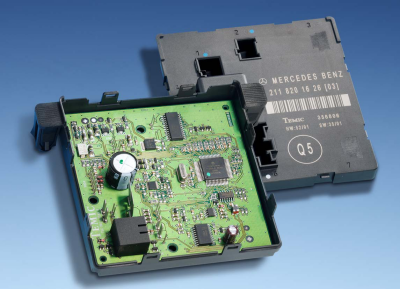
\includegraphics[width=8cm, 		   			height=5.5cm]{Images/image3.png} }}%
    \qquad
    \subfloat[\centering Undistorted image]{{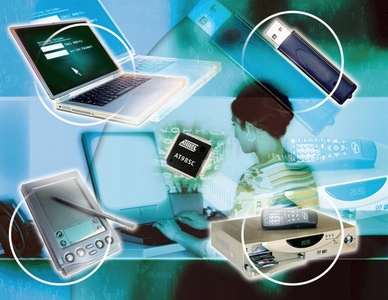
\includegraphics[width=8cm, height=5.5cm]{Images/image4.png} }}%
    \qquad
     \subfloat[\centering Car with $>$ 100 ECUs]{{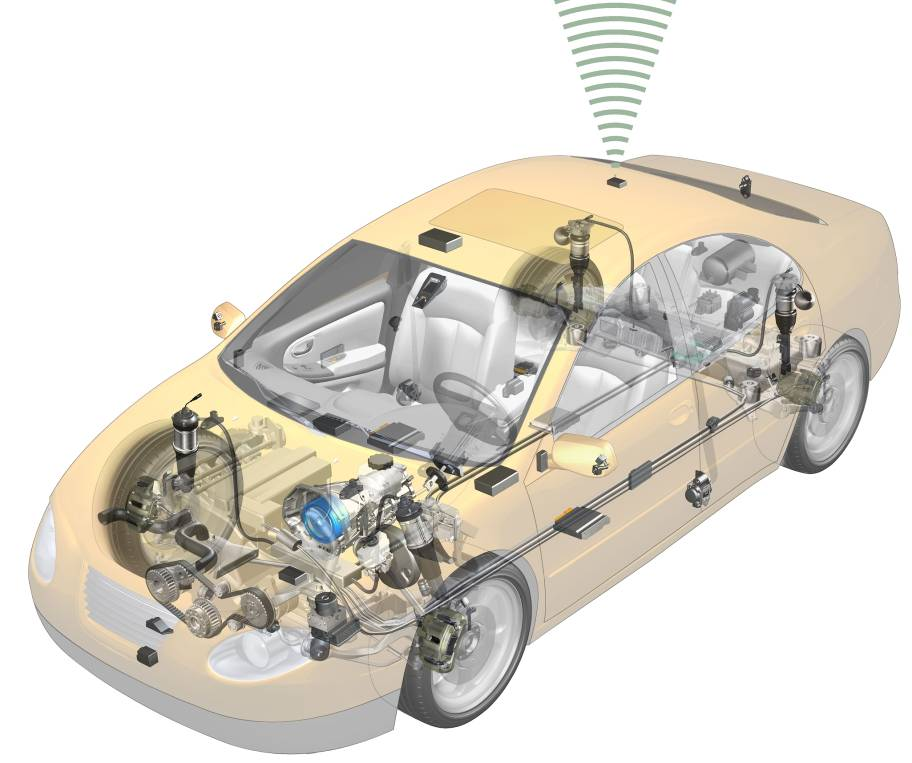
\includegraphics[width=7cm, height=5.5cm]{Images/image5.png} }}%
    \qquad
    \subfloat[\centering Pacemaker]{{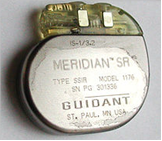
\includegraphics[width=6cm, height=5cm]{Images/image6.png} }}%
    \qquad
     \subfloat[\centering A319 Cockpit]{{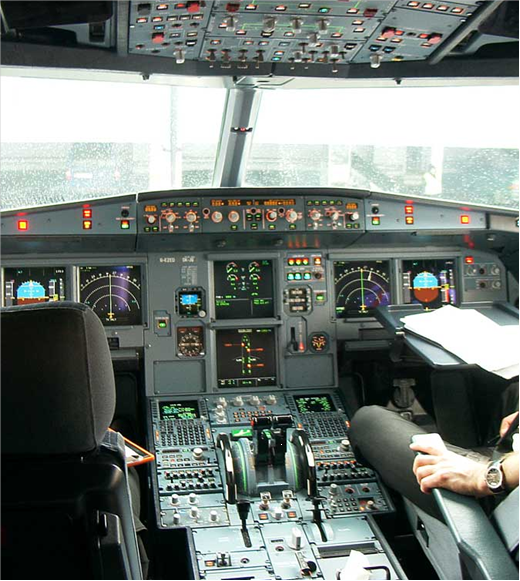
\includegraphics[width=8cm, height=5cm]{Images/image8.png}}}%
    \qquad
    \subfloat[\centering wikipedia.de: Arc welding of metal parts with industrial robots (KUKA). IPC, PLC]{{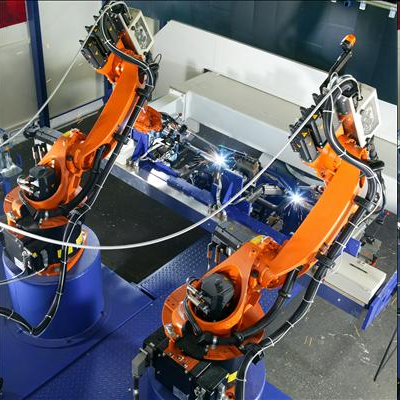
\includegraphics[width=8cm, height=5cm]{Images/image7.png} }}%
    \qquad
    \caption{ Comparison of results of video 1 (checkerboard000)}%
    \label{v1}%
\end{figure}


\begin{itemize}
	\item Examples of the use of real-time systems are found in the following areas: 
	\begin{enumerate}
		\item  Production 
		\item  Aerospace 
		\item  Automotive Electronics
		\item  Medicine
		\item  Military Technology, 
		\item  e-Banking, 
		\item  e-Trading, 
		\item  Telecommunications, 
		\item  Network Management, 
		\item  Power Generation/Management, 
		\item  Navigation
	\end{enumerate}
\end{itemize}

\textbf{The} need for Software\textbf{(mainly C-Code)in all areas of application grows rapidly}. 

\begin{tcolorbox}[colback=blue!5!white,colframe=blue!75!black]
  Moore's Law: “die Anzahl der Transistoren pro Chipfläche verdoppelt sich alle 2 Jahre”
\end{tcolorbox}

\begin{figure}[h]
    \centering
    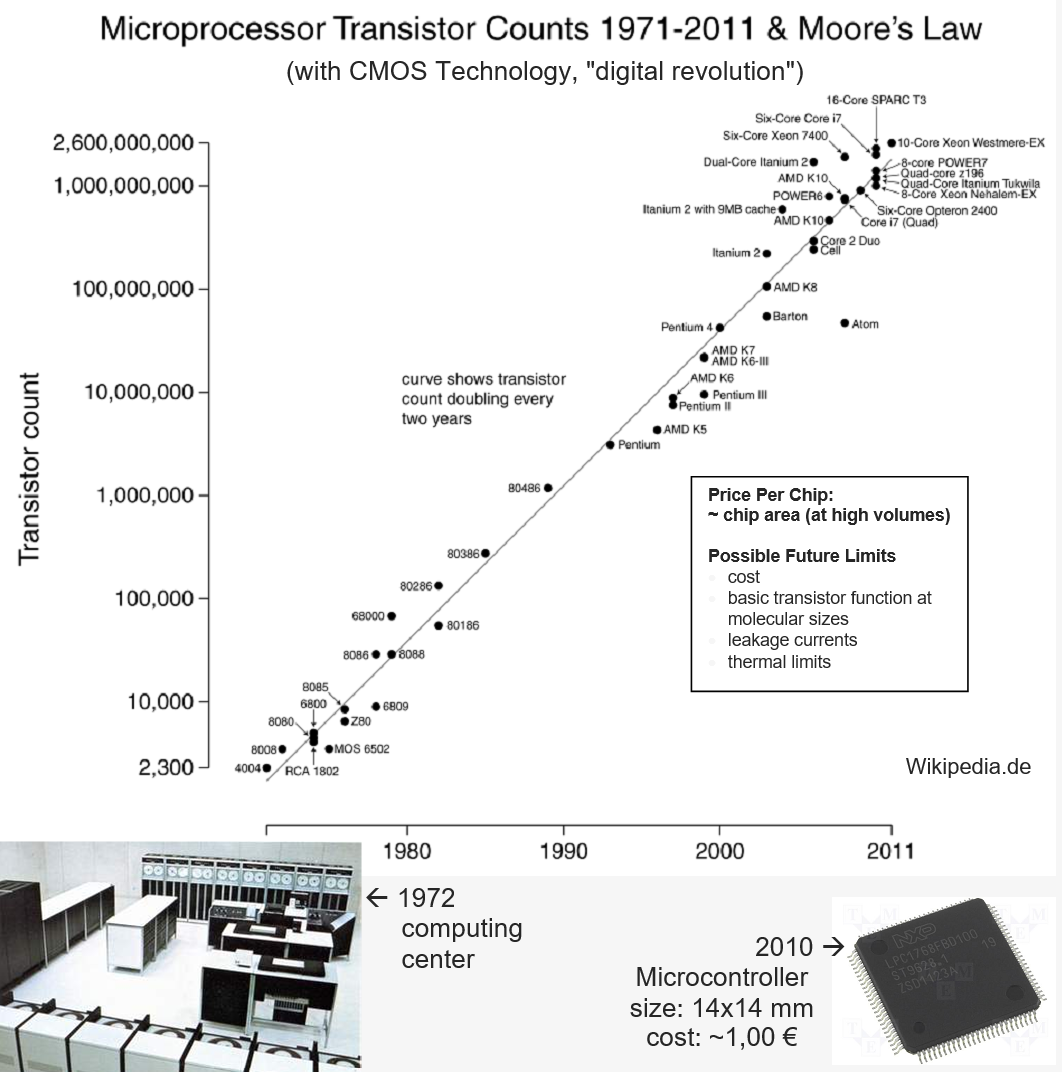
\includegraphics[width=13cm, height=10cm]{Images/image9.png}
    \caption{Moore's Law}
    \label{fig:Fig 3}
\end{figure}

\textbf{ Software for Real-Time Systems} differs substantially from software for generalpurpose computers (PC) due to the \textbf{requirements on the real-time behavior} !\\

Many methods of \textbf{classical software development} of non-real-time systems can not be used due to the lack of predictability.\\

For the development of real-time systems, special methods are required.\\


\section{ Requirements}

\newpage The validity of an operation of a real-time system depends on

\begin{enumerate}
	\item  its logical result, and
	\item  the physical time this result is available
\end{enumerate}

\begin{figure}%
    \centering
    \subfloat[\centering logical correct, but timing incorrect]{{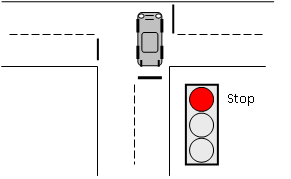
\includegraphics[width=7cm, 		   			height=5cm]{Images/image10.png} }}%
    \qquad
    \subfloat[\centering logical correct, and timing correct]{{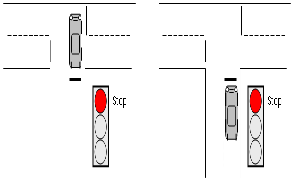
\includegraphics[width=7cm, height=5cm]{Images/image11.png} }}%
    \qquad
    %\caption{ Comparison of results of video 1 (checkerboard000)}%
    \label{fig:Fig 3}%
\end{figure}

\textbf{The traffic light control must determine traffic light phases logically and temporally correct.}\\

For real-time systems, the logical correctness \textbf{and} the timing correctness is required.

\begin{itemize}
	\item \textbf{Non Real-Time Systems}:  logical correctness  \textbf{OK}
	\item \textbf{Real-Time Systems}:    logical correctness + timing correctness  \textbf{OK}
\end{itemize}

\textbf{Example}: Real-Time Requirements with a Traffic Light Control

\begin{figure}[h]
    \centering
    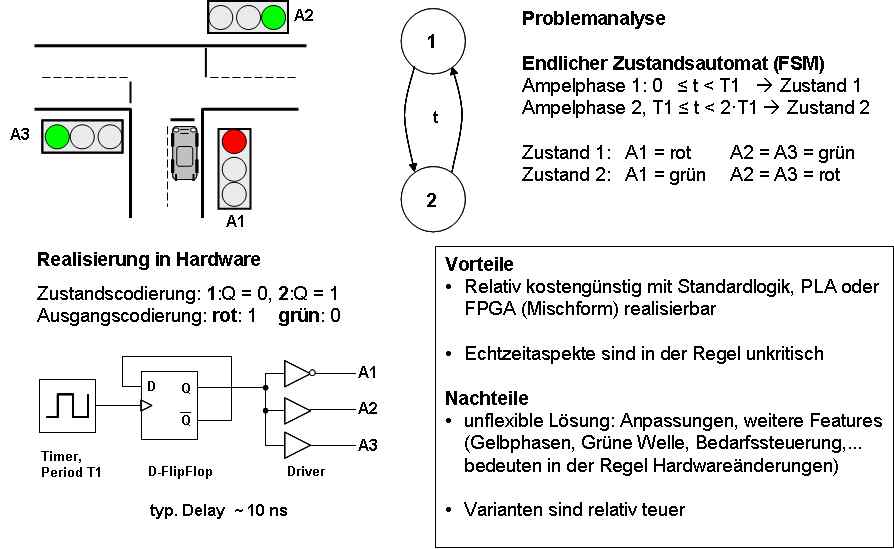
\includegraphics[width=14cm, height=9cm]{Images/image12.png}
    %\caption{Moore's Law}
    \label{fig:Fig 3}
\end{figure}

\begin{figure}[h]
    \centering
    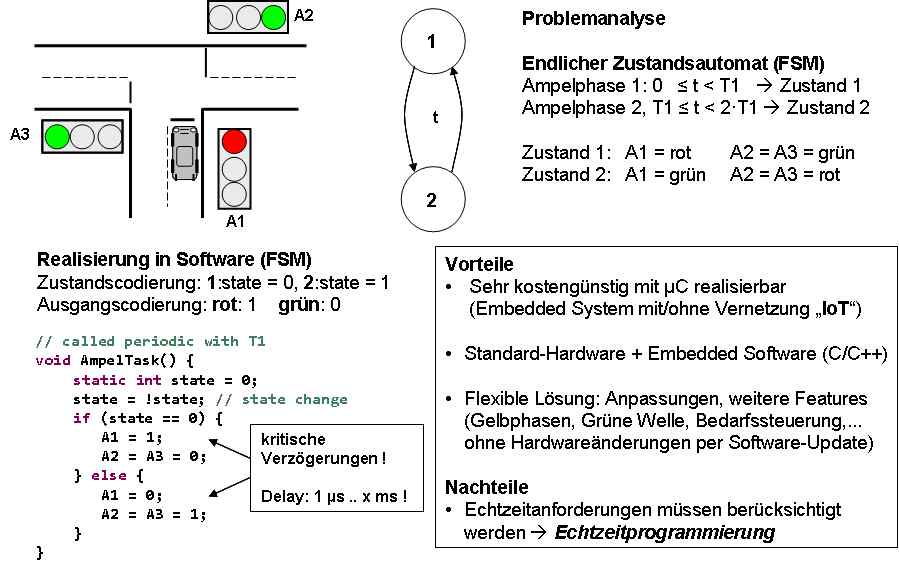
\includegraphics[width=14cm, height=8cm]{Images/image13.png}
    %\caption{Moore's Law}
    \label{fig:Fig 3}
\end{figure}

\begin{figure}[h]
    \centering
    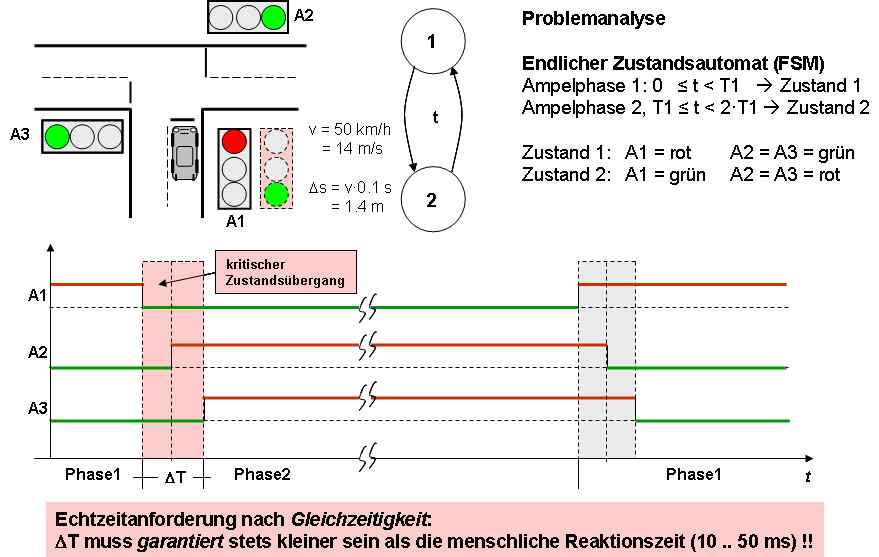
\includegraphics[width=14cm, height=8cm]{Images/image14.png}
    %\caption{Moore's Law}
    \label{fig:Fig 3}
\end{figure}

\newpage
\textbf{Solution}: Critical Section (Mutex) in AmpelTask:  see FSM Exercise

\begin{lstlisting}[style=mystyle, language=c]
 	// called periodic with T1  
	void AmpelTask() {
	static int state = 0;
	state = !state; // state change
  	begin(mutex);
	if (state == 0) {
		A1 = 1;
		A2 = A3 = 0;
	} else {
		A1 = 0;
		A2 = A3 = 1;
	}
  	end(mutex);
\end{lstlisting}

\newpage

{\rot\bf A Definition of Real-Time Systems is given by DIN 44300 [1985]}\\

\textit{ Realzeit-Systeme beziehungsweise Echtzeitsysteme sind Computersysteme, dieim Realzeitbetrieb arbeiten.}\\

\textit{Realzeitbetrieb wird definiert als der Betrieb eines Rechensystems, beidem Programme zur Verarbeitung anfallender Daten st\"{a}ndig betriebsbereitsind, derart, dass die Verarbeitungsergebnisse innerhalb einer vorgegebenenZeitspanne verf\"{u}gbar sind. Die Daten k\"{o}nnen je nach Anwendungsfall nacheiner zeitlich zuf\"{a}lligen Verteilung oder zu vorherbestimmten Zeitpunktenanfallen.}\\

{\rot\bf Wikipedia:}\\

In computer science, \textbf{real-time} computing (RTC), or reactive computing, is the study of hardware and software systems that are subject to a "real-time constraint", i.e., operational \textbf{deadlines} from \textbf{event to system response}. \\

By contrast, a \textbf{non-real-time system}  is one for which there is \textbf{no deadline}, even if fast response or high performance is desired or preferred. \\

The needs of real-time software are often addressed in the context of real-time operating systems, and synchronous programming languages, which provide frameworks on which to build real-time application software.\\

A real time system may be one where its application can be considered (within context) to be mission critical. \\

The anti-lock brakes on a car are a simple example of a real-time computing system - the real-time constraint in this system is the short time in which the brakes must be released to prevent the wheel from locking. \textbf{Real-time computations} can be said to have \textbf{failed if} they are \textbf{not completed before their deadline}, where their deadline is relative to an event. \\

\textbf{A real-time deadline must be met, regardless of system load}.\\

Thus, in a real-time system the logical correctness (functional correctness) of the answers with guaranteed response times (temporal correctness) is of essential importance. \\

The temporal behavior in real-time systems is part of the system specification and thus subject of the product verification.\\

\textbf{Embedded systems} often have to meet \textbf{real-time requirements}.\\

{\rot\bf Technical Process and Process Model}\\

A technical process can be defined as follows (DIN 66 201):\\

In a technical process materials, energy or information (the process media) are converted or transported (such as an end product) into grafted materials, energy or information. \\

Its input and state variables summarized in the vector \textbf{Z} can be measured with sensors and controlled by actuators: \\

\begin{figure}[h]
    \centering
    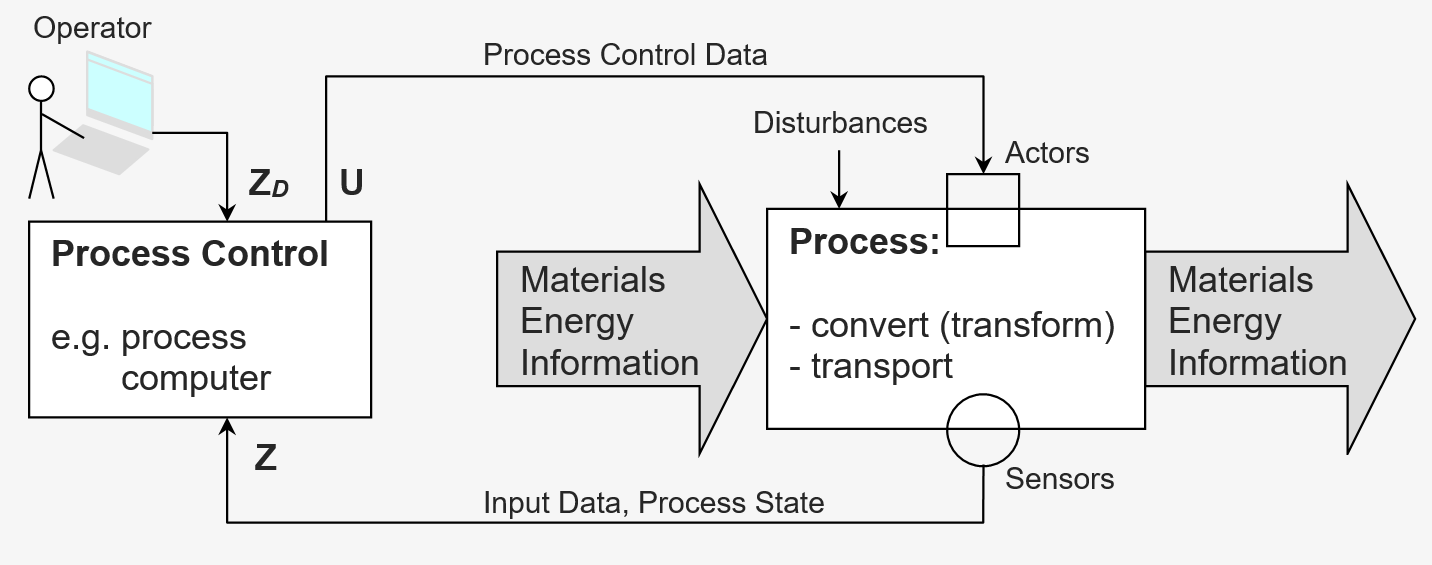
\includegraphics[width=14cm, height=6cm]{Images/image60.png}
    %\caption{Moore's Law}
    \label{fig:Fig 3}
\end{figure}

In automation, the process is controlled via control actions (vector \textbf{U}) so that after a given time, a desired process target or a desired state \textbf{Z\textit{${}_{D}$}} is reached. \\

The desired state can refer to the following:\\

quality, quantity (of the final product), speed, stability, security (during the transforming process), production, yield, raw material consumption, emissions, or even reaching the next process step (e.g. with sequential processes).\\

The delay time in the loop is of \textbf{\textit{crucial importance}} for the \textbf{\textit{stability}} of the \textbf{\textit{entire system}}!\\
This delay time must therefore be exactly specifiable  \textbf{\textit{Real-Time Programming}} !

\paragraph{  Timeliness}

The timeliness (=timing correctness) is directly derivable from the above considerations requirement for all real-time systems. For digital process computers timing correctness is, the output data must be calculated in time.

This also requires that the input data must be collected on time. The timing deadlines, and are usually given by a technical process:

Thus the allowed response time for the controller is limited to a known value, thus real-time systems are said to be \textbf{predictable} or \textbf{deterministic}.

Input data must be read in time for a real-time system, and the output data to be generated must be provided within the given deadline (time condition). 

The primary requirement for a real-time control is the \textbf{constant ability to input, process and output data on time regardless of the system workload}. 

For a real-time system also means that it \textbf{monitors the temporal validity} of information and prevents the use of invalid data !

This must apply regardless of whether the data to be processed are \textbf{event based} or at \textbf{predetermined (e.g. periodic) times}.

However, due to complexity, the timing behavior of real-time systems \textbf{can never be predicted with 100~\% certainty}  System validation by tests !

\paragraph{  Time Conditions}

The \textbf{time conditions} to monitor, and control a process can be in several variants

\begin{enumerate}
\item  Precise Time, Exact Time A precise time \textit{t}${}_{0}$ for a controller action is defined. This action must not be executed earlier or later. \textbf{Examples}: Sampling Systems (DSP \& Digital Control),      clock display control.

\item  Latest Time Limit, DeadlineA maximum time \textit{t}${}_{max}$ (=deadline) for a controller action is defined. This action must be finished latest at its deadline, but it can be finished earlier. \textbf{Examples}: a sampling system calculating an output sample for the next sampling      period, Anti-Squeeze Control, maximum response time with switching      on/off a machine, UI control reaction time to a button, slider, {\dots}      e.g. \textit{t${}_{max}$} $\mathrm{<}$ 50ms with human reaction times  ``\textit{immediately}''    

\item  Earliest Time Limit A minimum time \textit{t}${}_{min}$ for a controller action is defined. The action must not be executed earlier, but it can be executed later. \textbf{Examples}: transitions in state machines, an output may not occur before a state       transition has been finished.

\item  Time IntervalAn action must be executed within a time interval [\textit{t}${}_{min}$, \textit{t}${}_{max}$], thus at any time earlier than \textit{t}${}_{max}$ and later than\textit{ t}${}_{min}$. \textbf{Example}:  airbag ignition in some crash situations an airbag shall be ignited      e.g. 10-30 ms, in other situations 5-8 ms after crash.
\end{enumerate}

Time conditions can be \textbf{periodic} or \textbf{non-periodic}. 

\textbf{ Periodic Time Condition }

A periodic time condition is given with analog signals to be sampled and processed by a digital computer. Any analog signal has to be discretized in both value and time by a constant periodic sampling time \textit{T}${}_{s}$. This is typical for sampling systems realizing digital filters or digital control algorithms for processing quasi analog signals.

An example is the electric signal of a microphone which has to be sampled \textbf{strictly periodic} in order to have a \textbf{digital representation} of the \textbf{original analog sound signal}. Any deviation from the periodic sampling results in unwanted noise, which cannot be compensated. After time sampling the values of the voltage signal is discretized by an AD-Converter.

\textbf{Sampling Theorem [Kamm], [Oppen]}

\textbf{Example}: CD-Audio: \textit{f}${}_{s}$ = 44.1 kHz, \textit{T}${}_{s}$ = 22.7 µs  \textit{B${}_{x}$} = 20 kHz $\mathrm{<}$ 0.5 \textit{f}${}_{s}$ = 22.05 kHz 

Correct sampling:       tagesschau\_44.1.wav    Sampling theorem violation:  tagesschau\_D10.wav

Digital signal processing of analog signals involves very strict requirements to real-time conditions, due to the periodic and exact sampling conditions.

\begin{tabular}{|p{2.2in}|p{1.9in}|} \hline 
\textbf{Action} & \textbf{Time Condition} \\ \hline 
input of a sample of an analog signal    & exact periodic sampling at  k$\mathrm{\bullet}$\textit{T}${}_{s}$ \\ \hline 
computation of a signal sample  & time interval [k$\mathrm{\bullet}$\textit{T}${}_{s}$ + \textit{T${}_{ADC}$,} (k+1)$\mathrm{\bullet}$\textit{T}${}_{s}$] \\ \hline 
output of the calculated signal sample & exact periodic sampling at  (k+1)$\mathrm{\bullet}$\textit{T}${}_{s}$ \\ \hline 
\end{tabular}

\textbf{ Non-Periodic Time Condition}

A non-periodic time condition is given frequently with digital signals to be processed at arbitrary, non-predictable times due to events like pushing or releasing a switch or a revolution sensor, producing a slope at discrete angles of a motor shaft.

\textbf{Absolute Time Condition }With an absolute time condition defined, an action must be executed at a certain global time, i.e. an action must be performed at 12:00:00 MEZ.

\textbf{Relative Time Condition }With a relative time condition defined, an action must be executed relative to some previous event. Example: a control signal must be updated after 0.5~s after a push button was pressed.

All time conditions can arise in combinations.

For meeting the time conditions a real-time system must have

\begin{enumerate}
	\item  \textbf{sufficient processing speed} to process the input and output data at the required speed (sampling frequency), which the technical process requires
	\item  \textbf{deterministic time behavior}
\end{enumerate}

\paragraph{  Hard and Soft Real-Time Systems}

In the previous section, we saw that computation must complete before reaching a given deadline. In other words, real-time systems have timing constraints and are deadline-driven. Real-time systems can be classified, therefore, as either hard real-time systems or soft real-time systems.

What differentiates hard real-time systems and soft real-time systems are the degree of tolerance of missed deadlines, usefulness of computed results after missed deadlines, and severity of the penalty incurred for failing to meet deadlines.

For \textbf{hard real-time systems}, the level of tolerance for a missed deadline is extremely small or zero tolerance. The computed \textbf{results after} the \textbf{missed} \textbf{deadline} \textbf{are} likely \textbf{useless} for many of these systems. The penalty incurred for a missed deadline is \textbf{catastrophic} (e.g. an unstable control loop). 

For \textbf{soft real-time systems}, however, the level of tolerance is non-zero. The computed \textbf{results after} the \textbf{missed deadline} have a \textbf{rate of depreciation}. The \textbf{usefulness} of the results does \textbf{not reach zero immediately} passing the deadline, as in the case of many hard real-time systems. The physical impact of a missed deadline is\textbf{ non-catastrophic}.

\begin{enumerate}
	\item  \textbf{Hard Real-Time Conditions} the time conditions must be met, or catastrophes occur !  Deviations from the time-conditions are not allowed and represent a serious error. In safety-related systems a violation of the hard real-time time conditions can endanger human life (e.g. if sampling controls become unstable). Systems, meeting the hard real-time conditions are called \textbf{\textit{Hard Real-Time Systems}}. \textbf{Examples}: Sampling Controls (closed-loop), aerospace flight controls, airbag ignition, automotive X-by-wire, pacemakers, {\dots} 
	\item  \textbf{Soft Real-Time Conditions} the deadlines must be met but with a degree of flexibility. The deadlines can contain varying levels of tolerance, average timing deadlines, and even statistical distribution of response times with different degrees of acceptability. A missed deadline does not result in system failure, but costs can rise in proportion to the delay, depending on the application. Systems meeting soft real-time conditions are called \textbf{\textit{Soft Real-Time Systems}}.\textbf{Examples}: multimedia-streams (speech, video, music, low level audio), toasters, refrigerators, {\dots} 
\end{enumerate}

\paragraph{  Concurrency}

Real-time systems must generally treat multiple inputs and outputs simultaneously. Thus, the simultaneous addition to the timeliness of the second general requirement for real-time systems.

Example is about a CNC machine tool, where the x-y axes must be controlled simultaneously (synchronously, concurrently) to move the tool along a predetermined path \textit{B}(\textit{x}, \textit{y}) = \textit{B}(\textit{x}(\textit{t}), \textit{y}(\textit{t})). 

There is an relative time condition for both processes acting concurrently on the two drive axes x and y:

If the time axis of x and y are shifted by some amount of time $\Delta$\textit{T} (e.g. due to different clocks for x- and y-drive control), the resulting path \textit{B}(\textit{x}, \textit{y}) = \textit{B}(\textit{x}(\textit{t}), \textit{y}(\textit{t-}$\Delta$\textit{T})) will be wrong.

\textbf{Example}: Tolerances {\textbar}\textit{x}{\textbar}, {\textbar}\textit{y}{\textbar} $\mathrm{<}$ 0.05 mm,   Requirement    \textit{v${}_{x}$} = \textit{v${}_{y}$} = \textit{x}' = \textit{y}' = $\mathrm{\pm}$10 cm/s     Requirement     {\textbar}\textit{t}{\textbar} $\mathrm{<}$ {\textbar}\textit{x}{\textbar} / {\textbar}\textit{v${}_{x}$}{\textbar} = 0.5 ms       Synchronization, Real-Time Condition

\textbf{ Realizations of Real-Time Systems with Concurrency Requirement}

To meet the requirement of concurrency, there are several possibilities:

\begin{enumerate}
	\item  Full parallel processing in a multiprocessor system
	\item  Quasi-parallel processing in a multiprocessor system
	\item  Quasi-parallel processing in a uniprocessor system (\textbf{Multitasking})
\end{enumerate}

\begin{enumerate}
	\item  Each task is processed on a separate processor (e.g. microcontroller). There is a real parallel processing, each task has the full power of its own processor. This allows the independent consideration of each task, however, the tasks must be synchronized in most cases (e.g. x-y axis control of the CNC machine).
	\item  Each task executed on a processor that is allocated by a real-time scheduler(there are usually fewer processors available than tasks). The real-time scheduler is a hardware or software component, which assigns the tasks to processors such that all tasks can meet their timing constraints.The individual tasks can be assigned to single processors.
	\item  From a hardware perspective, the simplest and most cost effective and realization: All tasks share a single processor Multitasking. A Real Time Scheduler controls the allocation of the processor to the task. This form of real-time scheduling is the easiest to analyze and control  preferred realization of most embedded systems.
\end{enumerate}

\paragraph{  Availability}

Real-time systems must be available without interruption, otherwise time conditions may be violated. This leads to the third basic requirement of real-time systems, the \textbf{availability}. 

Real-time systems must be available over a longer period of time, maybe around the clock without any breaks, as with

\begin{enumerate}
	\item  Power Plant Controls
	\item  Production Facilities
	\item  Heating and Air Conditioning Systems
	\item  Communication
	\item  Medical Applications 
	\item  ...
\end{enumerate}

This requires that there is no disruption of operations for phases of system reorganization. A typical example here is the garbage collection of some programming languages such as Java or C \# or their runtime environments. For example, the default Java implementation is not suitable for use in real-time systems. Remedy is the use of algorithms free of need for reorganization (such as for dynamic memory management).

\textbf{Example}: Algorithm for Calculation of a Factorial in C OK with Real-Time programming      Not OK with Real-Time programming ! (Exec.-Time of stack operations not deterministic due to recursion). Another possibility is to divide the reorganization into small steps under control of the real-time scheduler to ensure that no time constraint is violated: This method is been used by Real-Time Java (Real-Time Specification for Java (RTSJ)).Also, more traditional memory management strategies involve not predictable time for execution (like \textbf{malloc/free} of the C standard library, \textbf{new/delete} with C++)  dynamic memory management is typically avoided with hard real-time systems !

\textbf{Example}:

Not OK with Real-Time programming     OK with Real-Time programming !(Exec.-Time of malloc() non deterministic)

- but: malloc() in initialization possible  

\subsection{  Timing Definitions}

\textbf{Process Time and Processing Time}

The time interval between two requests of the same type is called the \textbf{process time} \textit{T${}_{P}$}. If the interval between two events is constant, it is called a periodic event. 

In many cases, however, the time interval varies, so that there is a time interval with a minimum \textit{T${}_{Pmin}$} and a maximum \textit{T${}_{Pmax}$}.

For the actual processing of the event computer instructions (operations) have to be executed. The event belongs to the sequence of instructions is referred to as the code sequence or a job. Jobs are implemented within the computer as a computational process, which can be distinguished as \textbf{tasks} and \textbf{threads} (see section \textbf{Process Management}). 

For the execution of a job i the computer needs \textbf{processing time} \textit{T${}_{Vi}$} (from de: \textit{Verarbeitungszeit}) which is also called \textbf{execution time}.

The \textbf{processing/execution time }needed for a certain number of operations \textit{N} is inverse to the \textbf{computing power} \textbf{\textit{P}} (in ops / sec) a processor core (CPU) offers:

\begin{tabular}{|p{0.3in}|p{3.9in}|p{0.4in}|} \hline 
 & \textit{T${}_{V}$} = \textit{N} / \textit{P    }[\textit{T${}_{V}$}] = ops / (ops / sec) = sec\newline  & (1.1)
\end{tabular}

The CPU power is approximately proportional to the CPU clock frequency.

In practice it is not easy to specify the processing/execution time for a certain task, since it often depends on the input values (conditional branches). Furthermore, the performance of the processor varies (due to caches, pipelines and DMA). To calculate \textit{T${}_{Vmax}$} in real-time systems, \textit{N${}_{max}$} and \textit{P${}_{min}$} shall be used in \eqref{GrindEQ__1_1_}.

\textbf{Timeliness, Response time and Maximum Response Time}

Timeliness means, that a task required at the time \textit{t}${}_{0}$

\begin{enumerate}
	\item  is done \textbf{not before} a specified time \textit{t}${}_{0}$ + \textit{T${}_{Zmin}$} and
	\item  is done \textbf{no later} than a specified time \textit{t}${}_{0}$ + \textit{T${}_{Zmax}$} (timeliness).
\end{enumerate}

The requirement for a minimum latency, i.e, that a task is not been done before a certain time, is often missing (\textit{T${}_{Zmin}$} = 0) or can be realized easily. On the other hand, the requirement for \textbf{timeliness} (\textit{T${}_{R\ }$}$\mathrm{<}$ \textit{T${}_{Zmax}$}) is hard to guarantee. The \textbf{maximum reaction time} \textit{T${}_{Rmax}$} is the worst-case time when task execution ends and the computer can cause a reaction. The \textbf{maximum reaction time} \textit{T${}_{Rmax}$} always needs to be \textbf{smaller} than the \textbf{maximum response time} \textit{T${}_{Zmax}$}.

\textbf{Utilization, Load}

The computer core (CPU, processor) is loaded (utilized) depending on the frequency of occurrence of an event. The utilization  gives a relative measure how much the CPU is loaded by a task is the quotient of the necessary processing time \textit{T${}_{V}$} and process time \textit{T${}_{P}$}

\begin{tabular}{|p{0.3in}|p{3.9in}|p{0.4in}|} \hline 
 &  = \textit{T}${}_{V\ }$/ \textit{T}${}_{P}$ & (1.2) \\ \hline 
\end{tabular}

The total utilization ${}_{ges}$ is the sum of the utilization of all individual jobs \eqref{GrindEQ__1_3_}. A real-time system must be able to process all tasks with fulfilling their requirements for timeliness -- this is sometimes referred to as the requirement for concurrency (in a wider sense). Mathematically, this means that the total utilization \textit{${}_{ges}$} is less than 100\%:

\begin{tabular}{|p{0.3in}|p{3.9in}|p{0.4in}|} \hline 
 & $\begin{array}{l} {\rho _{ges} =\sum _{i=1}^{n}\rho _{i} = \sum _{i=1}^{n}\frac{T_{Vi} }{T_{Pi} }  } \\ {\rho _{ges} <\, \, 1} \end{array}$ & (1.3) \\ \hline 
\end{tabular}

\subsection{  Real-Time Evidence}

Evidence that all time requirements of all requests are met under all conditions, is very difficult (practically impossible). In principle, the real-time evidence is based on

\begin{enumerate}
	\item  evaluate the relevant characteristics of the technical process,
	\item  number of different requirements
	\item  Minimum processing time for each request
	\item  Minimum allowable response time for each request \textit{T${}_{Zmin}$}
	\item  Maximum allowable response time for each request \textit{T${}_{Zmax}$}
	\item  dependencies between events
	\item  identify the maximum processing time \textit{T${}_{VMax}$} (WCET = Worst Case Execution Time) for each request
	\item  check the\textbf{ load condition} \eqref{GrindEQ__1_3_}
	\item  verify the \textbf{timeliness condition} (determination of \textit{T${}_{Rmin}$} and \textit{T${}_{Rmax}$}).
\end{enumerate}

With verifying the \textbf{timeliness condition} in particular, it is not trivial to determine the maximum response time \textit{T${}_{Rmax}$}.

\textbf{ Estimate for the Worst Case Execution Time (WCET)}

The maximum processing time \textit{T${}_{VMax}$} -- often called Worst Case Execution Time (WCET) -- of a request is very difficult to determine. The WCET depends in particular on the algorithm, the implementation of the algorithm, the hardware used and the other activities of the system (other computing processes). Therefore, the WCET at best be estimated. In principle, two methods for determining the WCET can be distinguished:

\begin{enumerate}
	\item  measure the WCET 
	\item  static code analysis with WCET determination (count operations,cycle).
\end{enumerate}

\textbf{WCET Measure}

The WCET is determined by execution of the code sequence that will be processed, normally on the target platform. The time between the onset of the event and output at the end of the code sequence is determined. Condition: Modification of the real-time software

\textbf{Method for Measuring WCET}

To measure this time can be divided into two basic methods:

\begin{enumerate}
	\item  1st Measurement by the measure out piece of code itself (see above).The piece of code will be amended such that every time an event arrives and when the reaction took place, a time stamp\textit{ t}${}_{1}$ ( free running timer) is stored. At the end of the code, a second time stamp\textit{ t}${}_{2}$ is stored. the difference \textit{T${}_{Vi}$} = \textit{t}${}_{2}$ - \textit{t}${}_{1}$ is the actual execution timeThe first value \textit{T${}_{V}$}${}_{1}$ is stored as \textit{T${}_{Vmax}$}. With subsequent iterations, a newly calculated time \textit{T${}_{Vi}$}  is compared with the stored value. If the newly calculated time is greater than the previously measured WCET, the new value overwrites the existing WCET\textit{T${}_{Vmax}$} = max(\textit{T${}_{Vi}$})
	\item   External measurement of event and response (output), by means of an oscilloscope using port-toggle.
\end{enumerate}

For a WCET measure, appropriate input values and events must are generated. In addition, the entire system must be put under load (e.g. by an automatic tester).

\textbf{Advantages} of the method:

\begin{enumerate}
	\item  Independent of a programming language
	\item  Relatively easy to implement
	\item  Can run as autonomous self-diagnosis
\end{enumerate}

\textbf{Disadvantages} of the method:

\begin{enumerate}
	\item  The WCET of a code sequence can not be guaranteed, after all, it depends on many factors (background, loop iterations, caches, branches, etc ..).
	\item  The measurement is WCET is time consuming and ultimately expensive. Measure out the piece of code needs to be theoretically charged with all input data (in any combination).
	\item  This method can be carried out with the running code on the target platform only. Thus, an assessment at an early stage of development can be difficult.
	\item  A test environment is required (which provides the input data to create).
	\item  The code sequence to be measured out must be modified (for storing time stamps)  timers.
	\item  It is sometimes difficult to put the system under the required load.
\end{enumerate}

\textbf{ Static Code Analysis}

Here, the code itself is analyzed. Therefore most often an analysis tool program is used, which is fed with the object (machine) code, rather than with the C-source code. In addition, a hardware description is necessary (e.g. clock frequency of the microcontroller). 

The tool allows the duration of each code sequences to be estimated. After that, the number of loop iterations are considered, a bound of the number of cycles and the estimated execution time \textit{T${}_{SA}$} is printed.

Analysis can get rather complex, if cache hits, cache misses, processor pipelining are conssidered. 

If there are safety requirements, the code measured is not to changed after a static code analysis.

As a safety margin factors of \textit{c} = 2, 3, sometimes are used to state an upper limit

\textit{t}${}_{Vmax}$ $\mathrm{\le}$ \textit{T${}_{SA}$ }· \textit{c}

A manual determination of the number of cycles can be done in simple cases by inspection of the C-compiler generated assembler code:

Example: timer-interrupt routine for AVR microcontroller (e.g. ATmega8\_sum.pdf). The C-compiler generated assembly-/machine-code, ultimately determines the number of cycles to complete a section of code for a particular microcontroller (AVR here). The number of cycles multiplied by the instruction cycle time is the execution time.

\textbf{Estimation of the Best Case Execution Time (BCET)}

The determination Best Case Execution Time of a job can be done as the WCET, with the least possible load on the system, which can be easily implemented in general-at least in a test environment.

\textit{T${}_{Vmin}$} = min(\textit{T${}_{Vi}$})

\section{   Real-Time Operating Systems}

An \textbf{RTOS} (Real-time Operating System) must meet the same requirements as a standard general purpose operating system (GPOS) and offers services for


\begin{enumerate}
	\item  \textbf{Task Management}This is the management and organization of the implemented programs to be processed, also called tasks. The mission of the task management is thus essentially in the allocation of the processor (or the processors in a multiprocessor system) to the task.
	\item  \textbf{Resource Management}Tasks need resources for their execution, their allocation is the task of resource management. This mainly includes:- Memory management, responsible for allocating memory- Input/Output (I/O) management responsible for the allocation of I/O devices to  the tasks.
	\item  \textbf{Communication}The communication between tasks, called inter-process communication.
	\item  \textbf{Synchronization}A special form of communication is the synchronization, which refers to the timing of the tasks.
	\item  \textbf{Protection}The protection of resources against unauthorized access by tasks.
\end{enumerate}

These traditional requirements are exactly the same RTOSes as with GPOSes. Depending on the application, some of the services might be implemented only  rudimentary or completely absent. This is in particular with \textbf{embedded} \textbf{systems}, where the \textbf{RTOS} is kept as \textbf{lean as possible}, due to the limited resources.

In addition to the traditional OS requirements, real-time operating systems are required to 

\begin{enumerate}
	\item  Respect for timeliness and concurrency,
\end{enumerate}

\begin{enumerate}
	\item  Respect for availability.
\end{enumerate}

These requirements of RTOS dominate the other requirements, even if compromises are necessary.

\subsection{  Structure of an RTOS}

A real-time operating system (RTOS) is a program that schedules execution in a timely manner, manages system resources, and provides a consistent foundation for developing application code. Early operating systems had a monolithic structure, i.e. all functionality was implemented in a uniform, not further subdivided software block. This led to a number of disadvantages such as poor maintainability, poor adaptability and high error rate. Today's operating systems therefore follow a hierarchical layers model. 

\begin{enumerate}
	\item  \textbf{Device Driver}: This layer abstracts from the hardware, and- realizes the \textbf{hardware-dependent} \textbf{control} of each device - realizes the \textbf{hardware-independent} interface for the above layer. Ideally, the device drivers are the only hardware dependent layer in the OS. When adapting to other devices, only the device driver layer must be changed.
	\item  \textbf{I/O (Input-/Output) Control}, realizes the \textbf{logical}, \textbf{hardware-independent} device control. 
	\item  \textbf{Resource Management}: responsible for (allocation) and de-allocation (release) of memory and I/O resources.
	\item  \textbf{Task Management}: responsible for the allocation of the processor to each task. 
	\item  \textbf{API (Application Program Interface)} realizes the interface to the application.
\end{enumerate}

The OS kernel is critical for the stability and security, it is executed in the so-called \textbf{\textit{kernel mode}} of the processor, which allows full access to all resources.

The \textbf{\textit{kernel mode}} is a special operating mode of (advanced) microprocessors, enabling privileged instructions, direct access to memory and I/O, change configuration registers, etc.

In normal \textbf{\textit{user mode}} this privileged commands are blocked so that an application can not interfere with important operating system parts. This is one of the protection services of the operating system.

In the previous layer model, the core operating system extends over the layers 1 -- 4. Since the core contains many layers, it is called a \textbf{macro core operating system}.

Today's RTOSes must be highly configurable, especially in the field of \textbf{embedded systems} where scarce resources are typical  FreeRTOS.

It is therefore desirable to remove unwanted parts from the operating system, e.g. not needed scheduling or protection methods. This leads to the concept of the \textbf{micro-kernel operating system}.

\subsection{ Task Management}

The task management is a core task of operating systems. The most significant differences between standard and real-time operating systems are found here.

The tasks in a real-time application must meet the requirements for timeliness and concurrency. This requires scheduling strategies for RTOSes different from those found in  standard operating systems.

\paragraph{  Task Model}

A \textbf{computational process} or \textbf{process} (also called \textbf{task}) is running as a computer program together with all the variables (including register states) and resources each process has a \textbf{main()}

A task is a process controlled by the RTOS for execution of a sequential program. Several tasks are being processed by the quasi-parallel processor, necessary changes between tasks are made by the RTOS' task scheduler.

Changes between tasks are needed to meet all tasks requirements for timeliness.

Within a \textbf{\textit{process}}, there can be parallel \textbf{\textit{threads}} (running simultaneously). 

A \textbf{\textit{thread}} must share its resources with other \textbf{\textit{threads}} of the same \textbf{\textit{process}}  just${}_{\ }$1${}_{\ }$\textbf{main()}

\begin{enumerate}
	\item  A \textbf{task} is called a \textbf{heavyweight process, }if it contains its own variables and resources separated from other tasks by the OS. It has its own address space and can communicate with other tasks via interprocess communication. A task realized as a process provides maximum protection, possible interference by other tasks is limited to predefined channels. A change of the processor to another task (\textbf{context switch}) is due to the separate resources, which is a time-consuming task.
	\item  A \textbf{task} realized as a \textbf{thread} is called a \textbf{lightweight process} that exists within a single process. It uses the variables and resources of the process. All threads within a process \textbf{share the same address space}. Communication can take place over any global variable within the process. Threads can interfere with any other thread within a task.  Shared memory allows great efficiency. Communication between threads is more direct and faster Context switch can take place very quickly, e.g.: FreeRTOS, VxWorks Low data protection between data of individual threads
\end{enumerate}

To fulfill the \textbf{real-time requirements}, efficiency is usually more important than protection. 

Many real-time applications use \textbf{threads within a single task}.

Often, a real-time application is realized by a \textbf{\textit{single}} \textbf{\textit{process}}, which contains threads to realize numerous tasks.\textbf{ Embedded systems} are often based on the \textbf{thread concept}, due to scarce resources.

From the perspective of the real-time conditions (timeliness, concurrency, availability), \textbf{threads} aren't different from \textbf{processes}, both are usually identified by the term \textbf{task}.

\paragraph{ Multitasking, Context Switch }

Multitasking is the ability of the OS to handle multiple tasks within set deadlines. An RTOS kernel might have 2 tasks that it has to schedule to run. At certain times, execution of Task 1 has to switch to Task 2

\paragraph{  Task States}

For each task (or threads) one can define 6 different states:

\begin{enumerate}
	\item  \textbf{existent}
	\item \textbf{ ready (}waiting\textbf{)}The task is ready, all conditions are fulfilled, resources are allocated, the task is waiting for the allocation of the processor.
	\item  \textbf{running }(executing)The task is run on the processor. In a uniprocessor only one task can be in this condition, in a multi-processor system, several tasks can be in this state simultaneously. 
	\item  \textbf{blocked} (blocked)The task is waiting for an event (e.g. an input value, an inter-process communication object) or the release of a resource (task synchronization). 
	\item  \textbf{suspended }(finished)A task is suspended from its normal operations by another task. It can be resumed later
	\item  \textbf{not existent}
\end{enumerate}

\subsection{  Real-Time Scheduling}

The main job of an RTOS task management is the allocation of the processor to the ready tasks. There are different strategies, so-called scheduling strategies.

A \textbf{real-time scheduler} must divide all ready (runnable) tasks to the processor, so that all all time conditions are met. The set of tasks managed by the real-time scheduler is called \textbf{taskset}.

For the evaluation of various scheduling strategies, the processor demand \textit{H} (=\textbf{utilization}) is an important quantity for the load of the processor, it is defined as

\begin{tabular}{|p{0.3in}|p{3.9in}|p{0.4in}|} \hline 
 & \textit{\newline H} =\newline  & (2.1) \\ \hline 
\end{tabular}

Each CPU can be utilized up to 100 \% at maximum.\textbf{  Example}: A periodic task 1 with a period of \textit{T}${}_{P1}$ = 200 ms and an execution time of \textit{T}${}_{e1}$ = 100 ms causes a processor demand of \textit{H}${}_{1}$ = 50 \%

A second periodic task with a period of \textit{T}${}_{P2}$ = 100 ms and an execution time of \textit{T}${}_{e2}$ = 50 ms also causes a processor demand of \textit{H}${}_{2}$ = 50 \%. 

An implicit timing condition for each periodic task is: task execution must be finished before the next period starts (deadline) !

Both tasks cause a total processor demand \textit{H} = \textit{H}${}_{1}$ + \textit{H}${}_{2}$ = 100~\%.

One possible schedule for executing both tasks is to displace task 1 after exactly half of its execution time by task 2, which is never displaced. Thus, task 1 must be displaceable:

another possible schedule:

In general, for a tasklet of \textit{n} periodic tasks, the total processor demand

\begin{tabular}{|p{0.3in}|p{3.9in}|p{0.4in}|} \hline 
 &         $H=\sum _{i=1}^{n}\frac{T_{ei} }{T_{pi} }  $ & (2.2) \\ \hline 
\end{tabular}

\paragraph{  Classification of Scheduling Algorithms}

\textbf{Static Scheduling}

Prior to the execution of a taskset an allocation table (dispatching table) with the start times exists, regarding time constraints and dependencies of each task. The dispatcher as part of the RTOS kernel assigns the individual tasks due to this table 

 principle of synchronous programming.

Advantage  minimal overhead, as no decisions are needed at runtime. 

Disadvantage  restriction to periodic events.

\textbf{Dynamic Scheduling}

Here for the execution of tasks different criteria are used by the dispatcher \textbf{at runtime}, taking into account start times, time conditions (deadlines), and dependencies of each task. Asynchronous programming. Advantage  increased flexibility and the opportunity to respond to aperiodic events. Disadvantage  increased overhead, lower predictability

\textbf{Static and Dynamic Priorities}

(Not to be confused with static/dynamic scheduling). The scheduler can use priorities for the allocation of resources (processor, memory, I/O,{\dots}) to a task. \textbf{Static priorities} are set before running the application and are never changed during runtime. \textbf{Dynamic priorities} can be adjusted for each task \textbf{at runtime}. Furthermore, there are algorithms, using \textbf{No Priorities} at all. 

\paragraph{ Preemption}

(= "Prioritization") is an important feature for a scheduler, which describes the capability for displacing a running task for later execution in favor of another task. 

\textbf{Preemptive scheduling }means that a less important task can be displaced by a more important task. The most important task with \textbf{\textit{ready}}-state will be executed immediately. The less important task will be continued again until no other more important task waits with \textbf{\textit{ready}}-state.

\textbf{(a) Preemptive Scheduling          (b) Non-Preemptive Scheduling }

\textbf{Non-preemptive scheduling} (= \textbf{cooperative scheduling}) means, that there is no displacement of a running task. Only after the current task is finished or blocked, the next task with \textbf{\textit{ready}} state is executed.


\paragraph{  Time-Slice Scheduling (Round-Robin Scheduling)}

Time-Slice Scheduling (time slicing) assigns each task a fixed time slice (Time Slice). The order of task execution corresponds to the sequence of \textbf{\textit{ready}}-tasks entering the task-list of the OS scheduler (FIFO principle). The duration of the time slice for a task can be set individually.


This type of time-slice scheduling is a dynamic preemptive scheduling. 

 TSS does not use priorities

 time slot duration can be chosen individually for each task

 With time slices chosen fine-grained enough TSS is approaching optimality.

\textbf{Principle of Time-Slice (Round-Robin) Scheduling: }

\begin{enumerate}
	\item  All \textbf{\textit{ready}}-tasks are queued in a FIFO 
	\item  Each task \textit{i} gets assigned a time slice (time slice, quantum) \textit{T${}_{TSi}$}
	\item  If a task after the expiry of its quantum is still \textbf{\textit{running}},
	\begin{enumerate}
		\item  the task is preempted, i.e. displaced to the \textbf{\textit{ready}} state
		\item  the task is put at the end of the FIFO queue;
		\item  The first task in the FIFO will be executed.
	\end{enumerate}
	\item  If a task changes state from \textbf{\textit{blocked}} to \textbf{\textit{ready}}, it will be put at the end ofthe FIFO queue
\end{enumerate}

Typical Applications: \textbf{Kernel-mode programs  Example 1:} 3 Tasks with \textit{H}${}_{max}$ $\mathrm{<}$ 0.778, from [W\"{o}rnB] , same as in section 2.2.7: Task T1: period \textit{T}${}_{p1}$ = 10~ms, execution time \textit{T}${}_{e1}$ = 1~ms  \textit{H}${}_{1}$ = 0.1Task T2: period \textit{T}${}_{p2}$ = 10~ms, execution time\textit{ T}${}_{e2}$ = 5~ms  \textit{H}${}_{2}$ = 0.5Task T3: non-periodic, period \textit{T}${}_{p3}$ = deadline \textit{T}${}_{d3}$ = 15.4~ms, \textit{T}${}_{e3}$ = 2.62~ms  \textit{H}${}_{3}$ = 0.17

By \eqref{GrindEQ__2_2_} the total CPU utilization \textit{H} = 0.1 + 0.5 + 0.17 = 0.77 

One chooses a basic time-slice \textit{T}${}_{TS}$ = 1 ms and assigns individual time slices as multiples of \textit{T}${}_{TS}$ with $\Sigma$\textit{T}${}_{TS}$ = 9~ms:

Task T1:    \textit{T}${}_{TS1}$ = 1 $.$\textit{T}${}_{TS}$ = 1 ms  \textit{H}${}_{1}$ = \textit{T}${}_{TS1}$/$\Sigma$\textit{T}${}_{TS}$ = 1~ms / 9~ms = 11~\%

Task T2:    \textit{T}${}_{TS2}$ = 5 $.$\textit{T}${}_{TS}$ = 5 ms  \textit{H}${}_{2}$ = \textit{T}${}_{TS2}$/$\Sigma$\textit{T}${}_{TS}$ = 5~ms / 9~ms = 55~\%

Task T3:     \textit{T}${}_{TS3}$ = 3 $.$\textit{T}${}_{TS}$ = 3 ms  \textit{H}${}_{3}$ = \textit{T}${}_{TS3}$/$\Sigma$\textit{T}${}_{TS}$ = 3~ms / 9~ms = 33~\%

(a)

In this example the assigned time slices were chosen to be larger than the execution times of each task, in order to avoid preemption.

With TSS a context-switch can occur at the end of a time-slice only. which can cause some \textit{jitter} (as with task T1 above).

\paragraph{ Fixed Time-Slice-Scheduling }

FT scheduling is based on a TDMA approach, requires no priorities, and is therefore frequently used in embedded microcontroller applications without an operating system.

A strictly periodic schedule is created with a periodic time \textit{N·T${}_{TS}$}, i.e. with \textit{N} integer multiples of the basic \textit{T${}_{TS}$} time slice. Each task gets assigned one (ore more) basic time slots, large enough to hold the WCET of each:

Conditions for Events are polled within each task, if a task is not finished at the end of its timeslice, it can be preempted (\textbf{\textit{preemptive FTS}})or not (\textbf{\textit{cooperative FTS}}).

The previous example with three tasks, and an idle task T4 at a period \textit{N}$\mathrm{\bullet}$\textit{T${}_{TS}$} = $\Sigma$\textit{T${}_{TS}$} = 10 ms is realized, the time slices are chosen as multiples of \textit{T${}_{TS}$} = 1 ms as follows 

Task T1:    \textit{T${}_{TS}$}${}_{1}$ = 1 $.$\textit{T${}_{TS}$} = 1 ms  \textit{H}${}_{1}$ = \textit{T${}_{TS}$}${}_{1}$/$\Sigma$\textit{T${}_{TS}$} = 1~ms / 10~ms = 10~\%

Task T2:    \textit{T${}_{TS}$}${}_{2}$ = 5 $.$\textit{T${}_{TS}$} = 5 ms  \textit{H}${}_{2}$ = \textit{T${}_{TS}$}${}_{2}$/$\Sigma$\textit{T${}_{TS}$} = 5~ms / 10~ms = 50~\%

Task T3:     \textit{T${}_{TS}$}${}_{3}$ = 3 $.$\textit{T${}_{TS}$} = 3 ms  \textit{H}${}_{3}$ = \textit{T${}_{TS}$}${}_{3}$/2$\Sigma$\textit{T${}_{TS}$} = 3~ms / 10~ms = 30~\%

Task T4 (idle) \textit{T${}_{TS}$}${}_{4}$ = 1 $.$\textit{T${}_{TS}$} = 1 ms  \textit{H}${}_{4}$ = 10~\%

T3 runs for the second time at \textit{t} = 26 ms the delay of 10 ms does not result in a T3-deadline violation. The idle task T4 provides a placeholder for unused CPU load, which can be used in modern CPUs for power saving features.

\textbf{Advantage of fixed TSS}: the execution times can be defined exactly!

\paragraph{ Binary Fixed Time-Slice-Scheduling }

If task periodic times \textit{T${}_{Pi}$} can be represented as power-of-2 integer multiples of a basic time slice \textit{T${}_{TS}$}, one can obtain a periodic binary schedule:

If the maximum time of execution is \textit{T}${}_{TS}$ and equal for each task, the utilization for each task is 

\begin{tabular}{|p{0.3in}|p{3.9in}|p{0.4in}|} \hline 
 & $H_{i} =\frac{T_{ei} }{T_{pi} } =\frac{T_{TS} }{2^{i} \cdot T_{TS} } =2^{-i} $     $\sum _{i=1}^{N}H_{i} \stackrel{N\to \infty }{\longrightarrow}  \; 1$ & (2.3) \\ \hline 
\end{tabular}

Thus, the fastest task with periodic time \textit{T${}_{p}$}${}_{1}$ = 2$.$\textit{T}${}_{TS}$ is assigned 50~\% of the complete processing time, task 2 with periodic time \textit{T${}_{p}$}${}_{2}$ = 4$.$\textit{T}${}_{TS}$ gets assigned 25~\%, task 3 gets 12.5~\%, {\dots}

From \eqref{GrindEQ__2_3_} it shows, that the total utilization of \textit{H} aiming with an infinite number of tasks to 100\%, thus, there will be no overload situations, if all tasks meet their maximum execution time \textit{T${}_{TS}$} requirement (easily guaranteed with a preemptive schedule).

\textit{   T${}_{TS}$} $\mathrm{\ge}$ max(\textit{T${}_{e}$}${}_{1}$,\textit{ T${}_{e}$}${}_{2}$,\textit{ T${}_{e}$}${}_{3}$, ..)

With a non-preemptive schedule (cooperative task schedule) maximum execution times \textit{T${}_{ei}$} have to be determined carefully (WCET determination), such, that each task can complete execution within the basic \textit{T${}_{TS}$}. If a task gets delayed for some reasons (like high priority interrupts during execution) the complete schedule will get delayed.

\textbf{Advantages }

Binary fixed time-slice scheduling is

\begin{enumerate}
	\item  quite suitable with multirate sampling systems (e.g. oversampling, when integer multiples of a common sampling frequency are needed).
	\item  a very simple scheduling without priorities,
	\item  suitable in a non-preemptive realization for even small microcontrollers without OS. 
	\item  Time and duration of execution for each task is guaranteed (apart from interrupts)
\end{enumerate}

\textbf{Disadvantages }

\begin{enumerate}
	\item \textbf{ }Binary time-slice scheduling is not fully flexible with arbitrary periodic times and execution times
	\item  can turn into very complex software, especially with integrating tasks with execution time larger than \textit{T${}_{TS}$}.
\end{enumerate}



\textbf{Lab-Experiment}   \textbf{\underbar{AVR-Timer-Interrupts-(FTS-Scheduling)}}

\textbf{\underbar{Sketch for Arduino Nano}  (FixedTimeSlice.ino)}

\textbf{Example}: 4 periodic tasks (on an AVR µC, from section Digital PID Control with 4 Tasks) 

\textit{T${}_{p}$}${}_{1}$ = \textit{T${}_{p}$}${}_{2}$ = 1 ms, \textit{T${}_{p}$}${}_{3}$ = 16 ms, \textit{T${}_{p}$}${}_{4}$ = 8 ms

\textit{T${}_{e}$}${}_{1}$ = 50 µs, \textit{T${}_{e}$}${}_{2}$ = 0.3 ms, \textit{T${}_{p}$}${}_{3}$ = 40 µs, \textit{T${}_{p}$}${}_{4}$ = 40 µs

\textit{H}${}_{1}$ = 5 \%, \textit{H}${}_{2}$ = 30 \%, \textit{H}${}_{3}$ = 0.1/20 = 0.5 \%, \textit{H}${}_{4}$ = 0.05/20 = 0.25 \%  \textit{H} = 30.75 \%

Solution with Binary time-slice schedule with 3 Tasks, \textit{T${}_{TS}$} = 0.5 ms, \textit{T${}_{TS}$} $\mathrm{\ge}$ max(\textit{T${}_{ei}$}) = max(0.3, 0.05, 0.005 0.0025 ms) tasks with the same periodic times run in the same time-slice: T1 und T2 executed successively in the 2 Timeslice 2·\textit{T${}_{TS}$ }= 1 ms

\begin{tabular}{|p{0.2in}|p{0.2in}|p{0.1in}|p{0.1in}|p{0.1in}|p{0.1in}|} \hline 
\textbf{t/\textit{T${}_{Ts}$}} & \textbf{16} & \textbf{8} & \textbf{4} & \textbf{2} & \textbf{1} \\ \hline 
\textbf{0} & 0 & 0 & 0 & 0 & 0 \\ \hline 
\textbf{1} & 0 & 0 & 0 & 0 & 1 \\ \hline 
\textbf{2} & 0 & 0 & 0 & 1 & 0 \\ \hline 
\textbf{3} & 0 & 0 & 0 & 1 & 1 \\ \hline 
\textbf{4} & 0 & 0 & 1 & 0 & 0 \\ \hline 
\textbf{5} & 0 & 0 & 1 & 0 & 1 \\ \hline 
\textbf{6} & 0 & 0 & 1 & 1 & 0 \\ \hline 
\textbf{7} & 0 & 0 & 1 & 1 & 1 \\ \hline 
\textbf{8} & 0 & 1 & 0 & 0 & 0 \\ \hline 
\textbf{9} & 0 & 1 & 0 & 0 & 1 \\ \hline 
\textbf{10} & 0 & 1 & 0 & 1 & 0 \\ \hline 
\textbf{11} & 0 & 1 & 0 & 1 & 1 \\ \hline 
\textbf{12} & 0 & 1 & 1 & 0 & 0 \\ \hline 
\textbf{13} & 0 & 1 & 1 & 0 & 1 \\ \hline 
\textbf{14} & 0 & 1 & 1 & 1 & 0 \\ \hline 
\textbf{15} & 0 & 1 & 1 & 1 & 1 \\ \hline 
\textbf{16} & 1 & 0 & 0 & 0 & 0 \\ \hline 
\textbf{17} &  &  & 0 & 0 & 1 \\ \hline 
... &  &  &  &  &  \\ \hline 
\end{tabular}

\textbf{time-slice indexes}


\textbf{Proof for collision-free assignment of time-slice indexes } (with \textit{k},\textit{l} $\in$ \textbf{$\boldsymbol{\mathbb{Z}}$}  integers)

for some period \textit{N} we get time slices at indexes  \textit{n${}_{k}$}  =  \textit{k$\bullet$N  +  $\frac{N}{2} $}  e.g.: 2, 6, 10, 14, ..

thus, for period 2\textit{N} (next time slice) we get    \textit{m${}_{l}$} =  \textit{l$\bullet$}2\textit{N  +  N  }e.g.: 4, 12, 20, 28, ..

for a collision, we set \textit{n${}_{k}$} ${\mathop{=}\limits^{!}} $ \textit{m${}_{l}$}. Division by \textit{N} on both sides shows \textit{k} + 0.5 ${\mathop{=}\limits^{!}} $ 2$\mathrm{\bullet}$\textit{l} + 1, which has no solution with integers \textit{k} and \textit{l}, thus the above assignment is without any conflict all time slice indexes (proof by full induction) !


\paragraph{  FIFO Scheduling}

The name derives from the FIFO (first in, first out) principle of a waiting queue:    

\includegraphics*[width=3.78in, height=2.53in]{image16}

where elements put into a queue in a certain order of sequence, are taken out in the same order of sequence.With a \textbf{FIFO scheduler}, the tasks are processed in the same order in which they have taken the ready state.  An running task is not interrupted, it is a \textbf{non-preemptive}, \textbf{dynamic} scheduler.

Advantage:   very simple implementation, sometimes used in universal OS

Disadvantage:  bad real-time performance,        violations of time conditions even at low processing demands ( example)


\textbf{Example}: Two tasks with FIFO scheduling

Task 1: \textit{T}${}_{p1}$ = 150 ms, \textit{T}${}_{e1}$ = 15 ms   \textit{H}${}_{1}$ = 0.1

Task 2: \textit{T}${}_{p2}$ = 10 ms,  \textit{T}${}_{e2}$ = 1 ms    \textit{H}${}_{2}$ = 0.1

For both periodic tasks there is a time bound (deadline) with the next period. With \eqref{GrindEQ__2_2_}   \textit{H} = \textit{H}${}_{1}$ + \textit{H}${}_{2}$ = 0.1 + 0.1 = 0.2 

For 20~\% processor demand only, it should be easy to find a schedule for this taskset, but:

This simple example shows that even at a very low processor demand, a FIFO scheduler \textbf{cannot} \textbf{guarantee} compliance with the real-time conditions.


\paragraph{ Fixed-Priority Scheduling}

For fixed-priority scheduling, each task is assigned a fixed priority. The \textbf{\textit{ready}}-task with the highest priority waiting in the scheduler's queue is assigned to the processor.  fixed-priority scheduling is\textbf{ dynamic scheduling with static priorities}. (often used with interrupt processing of microprocessors, preemptive or non-preemptive):

\begin{enumerate}
	\item  \textbf{Fixed-Priority-Preemptive Scheduling (FPP)}If a \textbf{task with higher priority} than the currently running gets into the ready state, then the \textbf{current task is interrupted (displaced, preemted)} and the task with the higher priority is assigned to the processor immediately.
\end{enumerate}

\begin{enumerate}
	\item  \textbf{Fixed-Priority-Non-Preemptive Scheduling (FPN)}If a \textbf{task with higher priority} than the currently running gets into the ready state, then the \textbf{task is assigned} to the processor only \textbf{after the current task} is either \textbf{completed} or \textbf{blocked}.
\end{enumerate}


\textbf{Advantage}: with FPP, the compliance with the real-time conditions can be guaranteed (unlike to FIFO scheduling), if the priorities were assigned appropriate. 

The assignment of priorities to tasks is an important step in the development of a real-time application.

\textbf{Rate-Monotonic-Scheduling (RMS)}

For purely periodic applications, there is a rule, the so-called \textbf{rate-monotonic scheduling rule}, which states, that the priority of the tasks to be performed is inversely proportional to their periodic time:

\begin{tabular}{|p{0.3in}|p{3.9in}|p{0.4in}|} \hline 
 &       $PR_{i} \sim \frac{1}{T_{pi} } $ & (2.4) \\ \hline 
\end{tabular}

under the (rather idealized) conditions:


\begin{enumerate}
	\item  Preemptive scheduling is used
	\item  The periodic times \textit{T${}_{Pi}$} are constant 		
	\item  The time limits (deadlines) are equal to the periodic times \textit{T${}_{Pi}$}
	\item  The execution times are known and constant \textit{T${}_{ei}$}
	\item  The tasks are independent from each other (can not deadlock)
\end{enumerate}

\textbf{Example}: (same as with FIFO scheduling in section 2.2.6). Two tasks with Fixed-Priority-Preemptive Scheduling (FPP):

Task 1: \textit{T}${}_{p1}$ = 150 ms, \textit{T}${}_{e1}$ = 15 ms,   lower priority by   \eqref{GrindEQ__2_4_}

Task 2: \textit{T}${}_{p2}$ = 10 ms,  \textit{T}${}_{e2}$ = 1 ms   higher priority by \eqref{GrindEQ__2_4_}

The running task 1 is displaced with an event for task 2, which has higher priority (its state goes from \textbf{\textit{blocked}}  \textbf{\textit{ready}}), so that the deadline of task 2 is not violated (in contrast to FIFO scheduling).

Obviously,\textbf{ FPP scheduling} with \textbf{RMS} provides much better results than FIFO scheduling. 

In contrast, with \textbf{FPN}, the deadlines of task 2 would be violated !

In general

This also means that FPP scheduling with RMS always delivers an executable schedule, if one exists. However, the overall CPU utilization may not exceed \textit{H${}_{max}$ }([1], by Liu)

\begin{tabular}{|p{0.3in}|p{3.9in}|p{0.4in}|} \hline 
 &   $H_{\max } =n\cdot \left(2^{1/n} -1\right)=n\cdot \left(\sqrt[{n}]{2} -1\right)$ & (2.5) \\ \hline 
\end{tabular}

\begin{tabular}{|p{0.7in}|p{0.6in}|} \hline 
\textbf{\textit{n}} & \textbf{\textit{H${}_{max}$}} \\ \hline 
1 & 1.000000 \\ \hline 
2 & 0.828427 \\ \hline 
3 & 0.779763 \\ \hline 
4 & 0.756828 \\ \hline 
5 & 0.743492 \\ \hline 
10 & 0.717735 \\ \hline 
20 & 0.705298 \\ \hline 
50 & 0.697974 \\ \hline 
100 & 0.695555 \\ \hline 
1000 & 0.693387 \\ \hline 
10000 & 0.693171 \\ \hline 
\end{tabular}

The limit \eqref{GrindEQ__2_5_} can be used to examine the feasibility of a (periodic) taskset and to guarantee the conformance with all time limits.

FPP with RMS is very popular because of its simplicity. However, there are problems at very high utilization (beyond or near \textit{H${}_{max}$}) and with RMS at the same or nearly the same time periods, delivering same task priorities. Furthermore, there are sometimes difficulties in approaching non-periodic processes by periodic processes with sufficient precision.

\textbf{Example 1:} 3 Tasks with \textit{H}${}_{max}$ $\mathrm{>}$ 0.778, from [W\"{o}rnB] : Task T1: period \textit{T}${}_{p1}$ = 10~ms, execution time \textit{T}${}_{e1}$ = 1~ms  \textit{H}${}_{1}$ = 0.1Task T2: period \textit{T}${}_{p2}$ = 10~ms, execution time\textit{ T}${}_{e2}$ = 5~ms  \textit{H}${}_{2}$ = 0.5Task T3: non-periodic, deadline = \textit{T}${}_{d3}$ = 15.4~ms, execution time\textit{ T}${}_{e3}$ = 5.5~ms

By \eqref{GrindEQ__2_2_} the total CPU utilization \textit{H} = 0.1 + 0.5 + 0.357 = 0.957, amost 100 \% !But with \eqref{GrindEQ__2_5_} \textit{H} $\mathrm{>}$ \textit{H}${}_{max}$ $\mathrm{>}$ 0.78 deadlines will be violated with \textbf{FPP/RMS} with 3 tasks. 

FPP/RMS \textbf{can't deliver an executable schedule}, as this example shows:

By \eqref{GrindEQ__2_4_} one has 2 choices for assigning the priorities due to the equal periods \textit{T}${}_{p1}$\textit{ }and \textit{T}${}_{p2}$:

\textbf{Priority assignment (a)   Priority assignment (b)}

\begin{tabular}{|p{0.5in}|p{0.9in}|} \hline 
T1 & high priority \\ \hline 
T2 & medium priority \\ \hline 
T3 & low priority \\ \hline 
\end{tabular}

\begin{tabular}{|p{0.2in}|p{0.9in}|} \hline 
T2 & high  priority \\ \hline 
T1 & medium priority \\ \hline 
T3 & low priority \\ \hline 
\end{tabular}

In both cases there is a violation of the T3 deadline, if all tasks get \textbf{\textit{ready}} the same time at \textit{t} = 0: 

(a)


(b)


Of course, the violation of T3 deadline in the example above occurs due to the deliberate disregard of the load limit \textit{H${}_{max}$}, by \eqref{GrindEQ__2_5_}. If one meets the max. load requirement \textit{H} $\mathrm{<}$ 78\% (n = 3), there is violation of the T3 deadline.

However, with growing number of tasks the maximum load goes down as low as 70\% (from n $\mathrm{>}$ 10), which is surprisingly low.

Ideas to achieve higher processor loads lead to dynamic assignment of priorities.

 \textbf{Example 2:} 3 Tasks with \textit{H}${}_{max}$ $\mathrm{<}$ 0.778, from [W\"{o}rnB] : Task T1: period \textit{T}${}_{p1}$ = 10~ms, execution time \textit{T}${}_{e1}$ = 1~ms  \textit{H}${}_{1}$ = 0.1Task T2: period \textit{T}${}_{p2}$ = 10~ms, execution time\textit{ T}${}_{e2}$ = 5~ms  \textit{H}${}_{2}$ = 0.5Task T3: non-periodic, period \textit{T}${}_{p3}$ = deadline \textit{T}${}_{d3}$ = 15.4~ms, \textit{T}${}_{e3}$ = 2.62~ms  \textit{H}${}_{3}$ = 0.17

By \eqref{GrindEQ__2_2_} the total CPU utilization \textit{H} = 0.1 + 0.5 + 0.17 = 0.77 With \eqref{GrindEQ__2_5_} \textit{H} $\mathrm{<}$ \textit{H}${}_{max}$ = 0.78 deadlines will be not violated with FPP/RMS with 3 tasks:

By \eqref{GrindEQ__2_4_} one has 2 choices for assigning the priorities due to the equal periods \textit{T}${}_{p1}$\textit{ }and \textit{T}${}_{p2}$:

\textbf{Priority assignment (a)   Priority assignment (b)}

\begin{tabular}{|p{0.5in}|p{0.9in}|} \hline 
T1 & high priority \\ \hline 
T2 & medium priority \\ \hline 
T3 & low priority \\ \hline 
\end{tabular}

\begin{tabular}{|p{0.2in}|p{0.9in}|} \hline 
T2 & high  priority \\ \hline 
T1 & medium priority \\ \hline 
T3 & low priority \\ \hline 
\end{tabular}

In both cases there is no violation of the T3 deadline, even if all tasks get \textbf{\textit{ready}} the same time at \textit{t} = 0: 

(a)

(b)

If one meets the max. load requirement \textit{H} $\mathrm{<}$ 78\% (n = 3), there is violation of the T3 deadline.

However, with 3 tasks the maximum load allowed is as low as 77.8\% (for \textit{n} = 3), which is surprisingly low.

Ideas to achieve higher processor loads lead to dynamic assignment of priorities  next sections.

\paragraph{  Earliest-Deadline-First Scheduling (EDF)}

In Earliest-Deadline-First Scheduling (EDF) the Task Processor is granted to that \textbf{\textit{ready}}-task, which is closest to its time limit (deadline). This is achieved by assigning the task priorities according to the vicinity to the individual deadlines.

EDF is dynamic scheduling with dynamic priorities, either preemptive or non-preemptive

For \textbf{preemptive EDF scheduling} a context-switch is made, when a task with earlier time bound gets \textbf{\textit{ready}}. In \textbf{non-preemptive EDF scheduling} is the task with the shortest time interval ist executed only, if the currently running task is finished or blocked.

Preemptive EDF scheduling, is used more frequently than non-preemptive EDF scheduling, which is essentially only used when non-interruptible processes are to be managed, such as disk access.

\textbf{Advantage}: With \textbf{preemptive EDF scheduling }100 \% CPU utilization can be achieved. 

\textbf{Example} with 3 Tasks (same as in section 2.2.7): Task T1: period \textit{T}${}_{p1}$ = 10~ms, execution time \textit{T}${}_{e1}$ = 1~ms  \textit{H}${}_{1}$ = 0.1Task T2: period \textit{T}${}_{p2}$ = 10~ms, execution time\textit{ T}${}_{e2}$ = 5~ms  \textit{H}${}_{2}$ = 0.5Task T3: non-periodic, deadline = \textit{T}${}_{d3}$ = 15.4~ms, execution time\textit{ T}${}_{e3}$ = 5.5~ms(each periodic time is assumed to be deadline).

Again, by \eqref{GrindEQ__2_2_} the total CPU utilization \textit{H} = 0.1 + 0.5 + 0.357 = 0.957, almost 100 \% !

(at \textit{t} = 0, T1 and T2 have equal priorities, due to equal deadlines, in such a case, the scheduler decides randomly, e.g. for the task with the lower id)

It can be seen, that with EDF scheduling an executable schedule is found. 

Liu [W\"{o}rnB] shows, that EDF scheduling is an optimal scheduling with

\begin{tabular}{|p{0.3in}|p{3.9in}|p{0.4in}|} \hline 
 & \textit{ H} $\mathrm{<}$ 100~\%    for preemptive EDF scheduling & (2.6) \\ \hline 
\end{tabular}

\textbf{Advantage}: 

\begin{enumerate}
\item  as long as the processor utilization is less than 100 \% with a uniprocessor system, EDF  scheduling delivers an executable schedule and compliance with all time conditions is guaranteed.
\end{enumerate}

\textbf{Disadvantages:}

\begin{enumerate}
\item \textbf{ }increased computational complexity for the dynamic priorities needed at run time.

\item  the sequence of task assignment is difficult to control.

\item  the time of execution is difficult to control with fixed time requirements.
\end{enumerate}

\subsection{  Task-Synchronization and Communication}

As most of the resources may only be used exclusively, tasks that request these resources must be synchronized for exclusive use, sometimes with regard to some sequence of access. 

Thus, the OS provides \textbf{means for} \textbf{synchronization} either for 

\begin{enumerate}
\item  mutual exclusion, and 

\item  cooperation (sequence of access).
\end{enumerate}

\paragraph{ Synchronization }

The problem of synchronization of tasks arises when these tasks are not independent

from each other. Dependencies arise, when common resources are be used, then the access needs to be coordinated. Common resources may be

\begin{enumerate}
	\item  \textbf{Data}Multiple tasks read and write access to shared variable, like tables. (without synchronization, uncoordinated access could result in inconsistent data, e.g. when task 1 is reading values of a table, while another task 2 is updating that table partly.
\end{enumerate}

\begin{enumerate}
	\item  \textbf{Devices} Multiple tasks using common devices such as sensors or actuators. (again, coordination is necessary to not to send e.g. contradictional commands of two tasks to a stepper motor drive).
\end{enumerate}

\begin{enumerate}
	\item  \textbf{Programs} Several tasks share common programs, such as device drivers. Competing calls to a device driver must be assured to leave consistent application states.
\end{enumerate}

\textbf{ Example}: Two tasks compete for access to a data table:

task 1 is reading several temperature sensors, and stores these values in a table

task 2 is reading this table, and prints out the temperature distribution.

Without synchronization, this can lead to erroneous results if, for example task 1, the common table has not yet been fully updated, while task 2 accesses. Then, task 2 gets mixed new and old temperature values, which can lead to undefined states !

There are two basic types of synchronization:

\begin{enumerate}
\item  The \textbf{Mutual Exclusion }or shortly called \textbf{\textit{Mutex}}, ensures that access to a common resource is permitted only to one task at a time. 
\end{enumerate}

\textbf{Example:} of temperature measurement using the \textbf{mutex} synchronization.

\textbf{ }For the protection of the common temperature table, a \textbf{mutex} is defined, toexclude the possibility that both tasks \textbf{access} this resource simultaneously.Before entering the critical section a task tries to acquire the mutex from the OS. If the mutex is already occupied by the other task, the newly accessing task is blocked\textbf{\textit{ }}until the other task \textbf{releases} the \textbf{mutex} again. The task will \textbf{un-block,} acquisition of the \textbf{mutex} succeeds, allowing the task to enter the critical section.The sequence, which task 1 or 2 acquires the \textbf{mutex} does not matter.


\begin{enumerate}
\item   Synchronization, where the order of access to common resources matters is called \textbf{cooperation} --unlike as with\textbf{ mutex synchronization}, which doesn't regard the order of task requests.
\end{enumerate}

Both, mutex synchronization and cooperation objects can be realized with semaphores.

\paragraph{ Semaphores}

A semaphore (from the Greek $\sigmaup$ $\muup$ $\alphaup$ = "sign" and $\varphiup$ $\varepsilonup$ $\rhoup$ $\varepsilonup$ $\iotaup$ $\nuup$ ="carry") is historically a signal mast or flag signal, in Information Technology it is an object for synchronization of processes.


A \textbf{semaphore} is basically a counter variable and two non-interruptible \textbf{operations}:  

\begin{enumerate}
\item  \textbf{Acquire}   (also called "\textbf{take}", "\textbf{signal}",  "\textbf{lock}",     or "\textbf{Passieren}", (\textbf{P}))

\item  \textbf{Release}  (also called "\textbf{give}", "\textbf{wait}",  "\textbf{unlock}"  or "\textbf{Verlassen}", (\textbf{V}))
\end{enumerate}

If a task tries to \textbf{\textit{acquire}} a semaphore, an associated counter variable is decreased. As long as the counter variable has a value less than 0, then the acquiring task is blocked.

Thus, during initialization the positive value of the semaphore states the number of tasks -waiting in a FIFO queue, or in a list using priorities- that may pass the semaphore, and thus enter the critical region protected by the semaphore.

If a task \textbf{\textit{releases}} a semaphore the associated counter variable is increased again. If the value of the counter variable is smaller than 1, tasks trying to acquire the semaphore are blocked, or, if the counter is greater or equal than 1, a waiting task is released from its blocking state  the task gets ready.Thus, a negative semaphore counter value indicates the number of tasks that have been prohibited to pass a semaphore. \textbf{Binary semaphore} only use \textbf{0} and \textbf{1} as counter values.

It is of crucial importance that the operations "Passieren" and "Verlassen" (as originally introduced by Dijkstra) are realized atomically, i.e. they cannot be interrupted by any other operation. Only then, a consistent handling of the counter variable is ensured. Semaphore objects are managed by the RT-OS.

\textbf{Other names} for the \textbf{semaphore operations}:

P(sem) = Passieren(sem) = sem.P() = sem.decrement() = sem.wait() = take(sem)${}_{VXWorks}$

V(sem) = Verlassen(sem) = sem.V() = sem.increment()  = sem.signal() = give(sem)${}_{VXWorks}$

\begin{enumerate}
\item  For \textbf{mutex-synchronization} a semaphore is used, with counter initialized with 1. Therefore, only one task can pass, gaining access to the protected resource: 
\end{enumerate}

\textbf{Example: Semaphore as Mutex in FreeRTOS}

\begin{enumerate}
\item  A \textbf{cooperation synchronization} can be realized by means of two semaphores. Example: sequential order of a task cooperation T2T1T2 with 2 semaphores:
\end{enumerate}

\textbf{Example: Cooperation in FreeRTOS  }


%%%%%%%%%%%%%%%%%%%%%%%%%%%%%%%%%%%%%%%%%%%%%%%%%%%%%%%%%%%%%%%%%%%%%%%%%%
\chapter{Real-Time Operating Systems}
An \textbf{RTOS} (Real-time Operating System) must meet the same requirements as a standard general purpose operating system (GPOS) and offers services for

\begin{itemize}
\item  \textbf{Task Management: }This is the management and organization of the implemented programs to be processed, also called tasks. The mission of the task management is thus essentially in the allocation of the processor (or the processors in a multiprocessor system) to the task.
\item  \textbf{Resource Management: }Tasks need resources for their execution, their allocation is the task of resource management. This mainly includes:- Memory management, responsible for allocating memory- Input/Output (I/O) management responsible for the allocation of I/O devices to  the tasks.
\item  \textbf{Communication: }The communication between tasks, called inter-process communication.
\item  \textbf{Synchronization: }A special form of communication is the synchronization, which refers to the timing of the tasks.
\item  \textbf{Protection: }The protection of resources against unauthorized access by tasks.
\end{itemize}

These traditional requirements are exactly the same RTOSes as with GPOSes. Depending on the application, some of the services might be implemented only  rudimentary or completely absent. This is in particular with \textbf{embedded} \textbf{systems}, where the \textbf{RTOS} is kept as \textbf{lean as possible}, due to the limited resources.\\

In addition to the traditional OS requirements, real-time operating systems are required to 

\begin{itemize}
	\item  Respect for \textbf{timeliness} and \textbf{concurrency}
	\item  Respect for \textbf{availability}
\end{itemize}

These requirements of RTOS dominate the other requirements, even if compromises are necessary.

\section{Structure of an RTOS}

A real-time operating system (RTOS) is a program that schedules execution in a timely manner, manages system resources, and provides a consistent foundation for developing application code.\\

Early operating systems had a monolithic structure, i.e. all functionality was implemented in a uniform, not further subdivided software block. This led to a number of disadvantages such as poor maintainability, poor adaptability and high error rate.\\

Today's operating systems therefore follow a hierarchical layers model. 

	\begin{figure}[h]
    \centering
    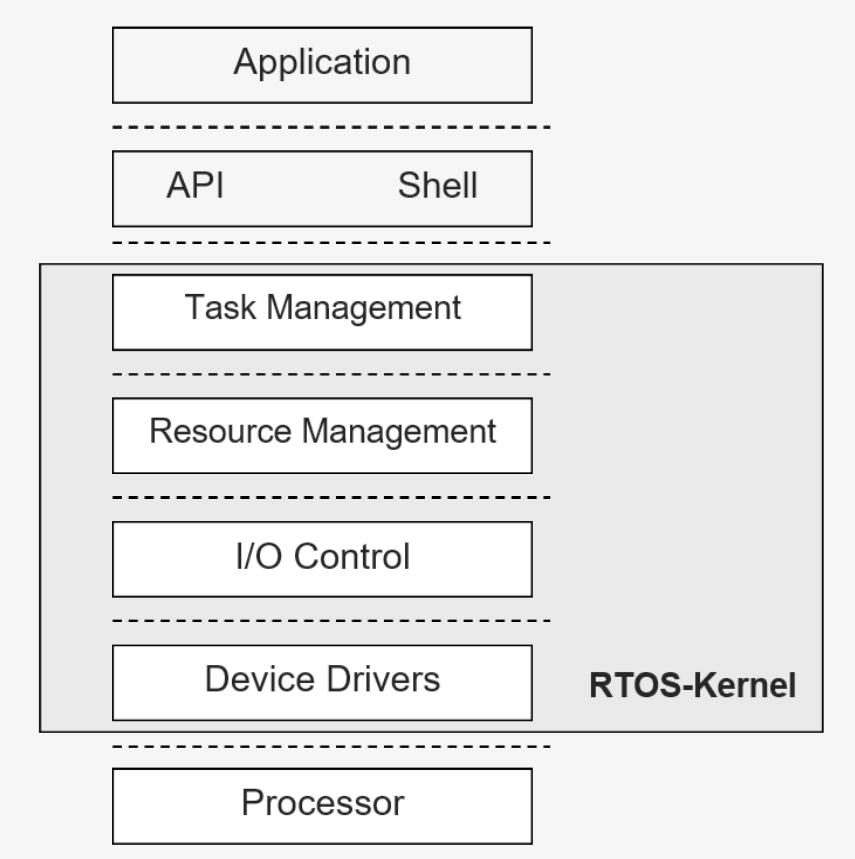
\includegraphics[width=9cm, height=7cm]{Images/image79.png}
    %\caption{}
    \label{fig:Fig 25}
    \end{figure}

\begin{itemize}
	\item  \textbf{Device Driver: } This layer abstracts from the hardware, and
	\begin{itemize}
		\item realizes the \textbf{hardware-dependent} \textbf{control} of each device
		\item realizes the \textbf{hardware-independent} interface for the above layer. 
	\end{itemize}

		Ideally, the device drivers are the only hardware dependent layer in the OS. When adapting to other devices, only the device driver layer must be changed.
	\item  \textbf{I/O (Input-/Output) Control}, realizes the \textbf{logical}, \textbf{hardware-independent} device control. 
	\item  \textbf{Resource Management: } responsible for (allocation) and de-allocation (release) of memory and I/O resources.
	\item  \textbf{Task Management: } Responsible for the allocation of the processor to each task. 
	\item  \textbf{API (Application Program Interface): } Realizes the interface to the application.
\end{itemize}

The OS kernel is critical for the stability and security, it is executed in the so-called \textbf{kernel mode} of the processor, which allows full access to all resources.\\

The \textbf{kernel mode} is a special operating mode of (advanced) microprocessors, enabling privileged instructions, direct access to memory and I/O, change configuration registers, etc.\\

In normal \textbf{user mode} this privileged commands are blocked so that an application can not interfere with important operating system parts. This is one of the protection services of the operating system.\\

In the previous layer model, the core operating system extends over the layers 1 -- 4. Since the core contains many layers, it is called a \textbf{macro core operating system}.

Today's RTOSes must be highly configurable, especially in the field of \textbf{embedded systems} where scarce resources are typical  $\rightarrow$ FreeRTOS.\\

It is therefore desirable to remove unwanted parts from the operating system, e.g. not needed scheduling or protection methods. This leads to the concept of the \textbf{micro-kernel operating system}.

\section{Task Management}

The task management is a core task of operating systems. The most significant differences between standard and real-time operating systems are found here.\\

The tasks in a real-time application must meet the requirements for \textbf{timeliness} and \textbf{concurrency}. This requires scheduling strategies for RTOSes different from those found in  standard operating systems.\\

{\rot\bf Task Model}\\

A \textbf{computational process} or \textbf{process} (also called \textbf{task}) is running as a computer program together with all the variables (including register states) and resources  $\rightarrow$ each process has a \textbf{main()}\\

A task is a process controlled by the RTOS for execution of a sequential program. Several tasks are being processed by the quasi-parallel processor, necessary changes between tasks are made by the RTOS' task scheduler.\\

Changes between tasks are needed to meet all tasks requirements for timeliness.

	\begin{figure}[h]
    \centering
    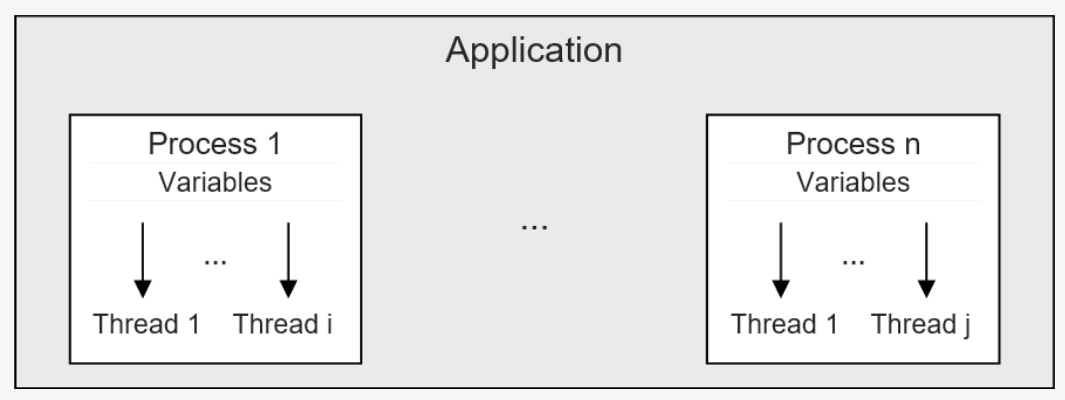
\includegraphics[width=10cm, height=4cm]{Images/image80.png}
    %\caption{}
    \label{fig:Fig 26}
    \end{figure}

Within a \textbf{\textit{process}}, there can be parallel \textbf{\textit{threads}} (running simultaneously). \\

A \textbf{\textit{thread}} must share its resources with other \textbf{\textit{threads}} of the same \textbf{\textit{process}} $\rightarrow$  just${}_{\ }$1${}_{\ }$\textbf{main()}\\

A \textbf{task} is called a \textbf{heavyweight process, }if it contains its own variables and resources separated from other tasks by the OS. It has its own address space and can communicate with other tasks via interprocess communication. \\

$\rightarrow$ A task realized as a process provides maximum protection, possible interference by other tasks is limited to predefined channels. \\

$\rightarrow$ A change of the processor to another task (\textbf{context switch}) is due to the separate resources, which is a time-consuming task.\\

A \textbf{task} realized as a \textbf{thread} is called a \textbf{lightweight process} that exists within a single process. It uses the variables and resources of the process. All threads within a process \textbf{share the same address space}. Communication can take place over any global variable within the process.

\begin{itemize}
	\item Threads can interfere with any other thread within a task.
	\item Shared memory allows great efficiency.
	\item Communication between threads is more direct and faster
	\item Context switch can take place very quickly, e.g.: FreeRTOS, VxWorks
	\item Low data protection between data of individual threads
\end{itemize}

To fulfill the \textbf{real-time requirements}, efficiency is usually more important than protection. \\

$\rightarrow$ Many real-time applications use \textbf{threads within a single task}.\\

Often, a real-time application is realized by a \textbf{\textit{single}} \textbf{\textit{process}}, which contains threads to realize numerous tasks.\textbf{ Embedded systems} are often based on the \textbf{thread concept}, due to scarce resources.\\

From the perspective of the real-time conditions (timeliness, concurrency, availability), \textbf{threads} aren't different from \textbf{processes}, both are usually identified by the term \textbf{task}.\\

{\rot\bf Multitasking, Context Switch }\\

Multitasking is the ability of the OS to handle multiple tasks within set deadlines. An RTOS kernel might have 2 tasks that it has to schedule to run. At certain times, execution of Task 1 has to switch to Task 2

	\begin{figure}[h]
    \centering
    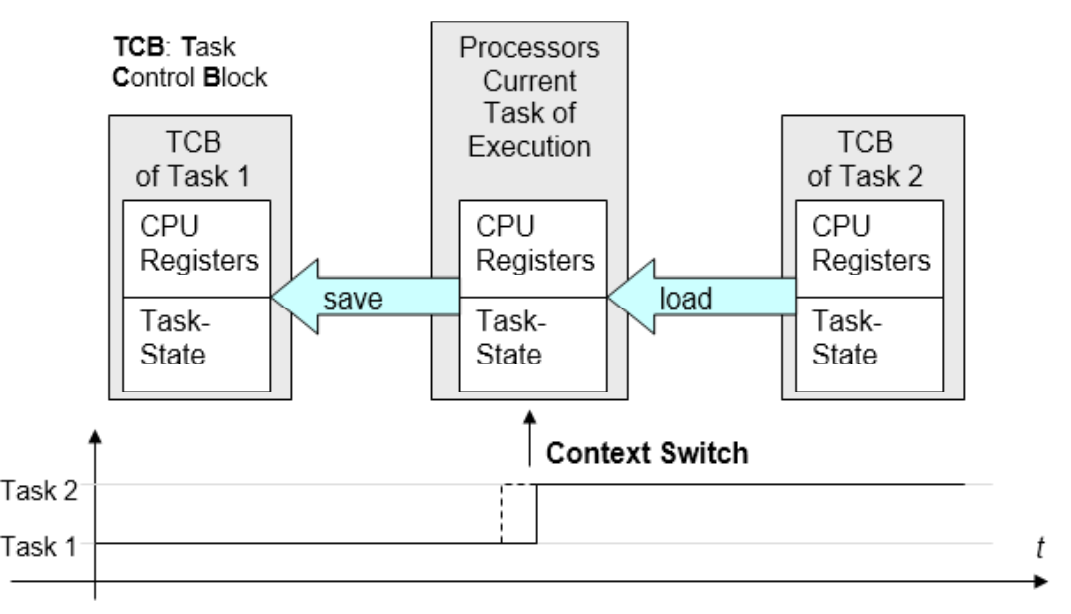
\includegraphics[width=13cm, height=6cm]{Images/image81.png}
    %\caption{}
    \label{fig:Fig 27}
    \end{figure}

{\rot\bf Task States}\\

For each task (or threads) one can define 6 different states:

	\begin{figure}[h]
    \centering
    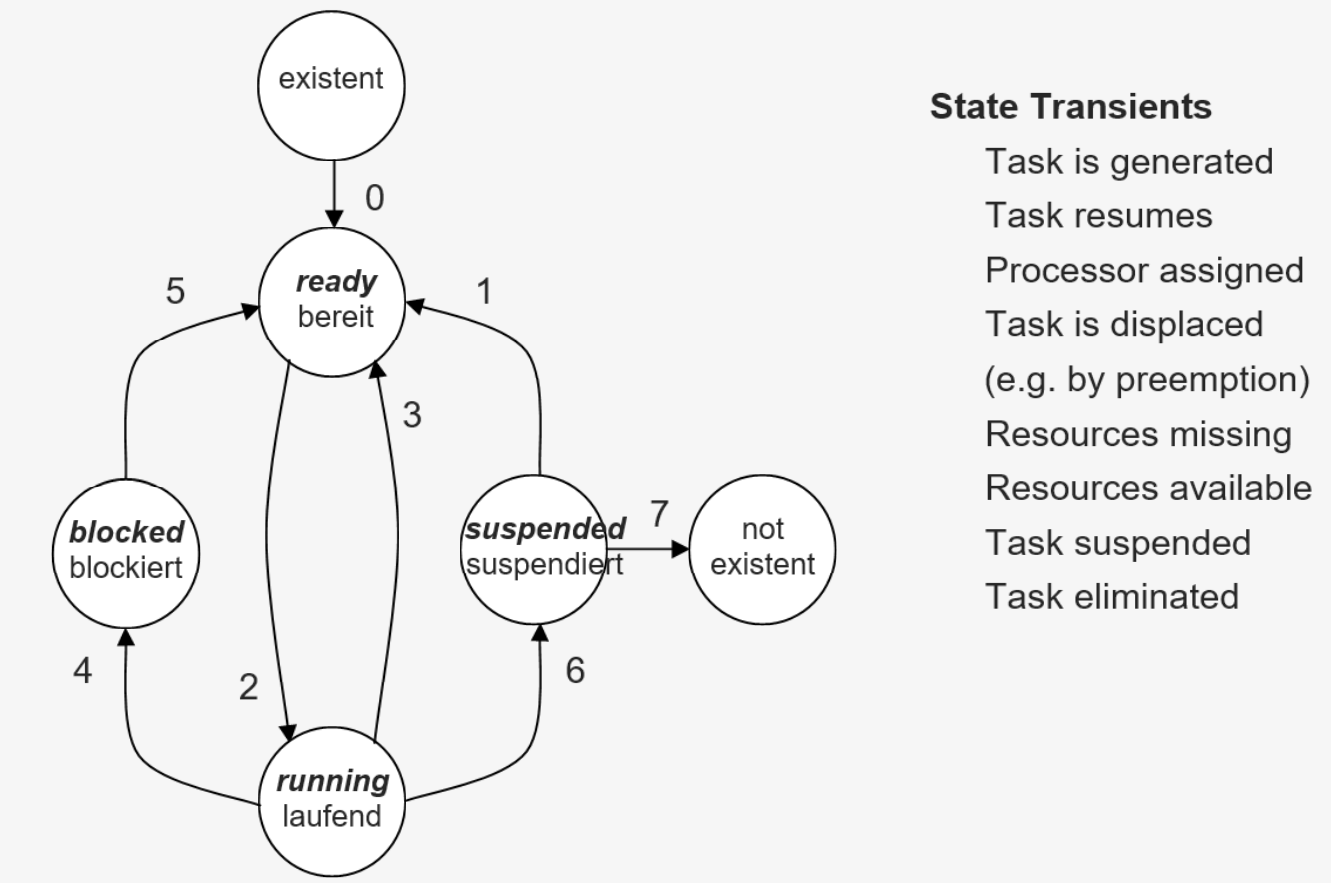
\includegraphics[width=13cm, height=8cm]{Images/image82.png}
    %\caption{}
    \label{fig:Fig 28}
    \end{figure}

\begin{itemize}
	\item  \textbf{existent}
	\item \textbf{ ready (}waiting\textbf{)}The task is ready, all conditions are fulfilled, resources are allocated, the task is waiting for the allocation of the processor.
	\item  \textbf{running }(executing)The task is run on the processor. In a uniprocessor only one task can be in this condition, in a multi-processor system, several tasks can be in this state simultaneously. 
	\item  \textbf{blocked} (blocked)The task is waiting for an event (e.g. an input value, an inter-process communication object) or the release of a resource (task synchronization). 
	\item  \textbf{suspended }(finished)A task is suspended from its normal operations by another task. It can be resumed later
	\item  \textbf{not existent}
\end{itemize}

\section{Real-Time Scheduling}

The main job of an RTOS task management is the allocation of the processor to the ready tasks. There are different strategies, so-called scheduling strategies.\\

A \textbf{real-time scheduler} must divide all ready (runnable) tasks to the processor, so that all all time conditions are met. The set of tasks managed by the real-time scheduler is called \textbf{taskset}.\\

For the evaluation of various scheduling strategies, the processor demand \textit{H} (=\textbf{utilization}) is an important quantity for the load of the processor, it is defined as

\begin{equation}
	H = \frac{Demanded Processor Time}{Available Processor Time}
\label{EQ 3}
\end{equation}
\newline
Each CPU can be utilized up to 100 \% at maximum.\\

\textbf{Example}: A periodic task 1 with a period of \textit{T}${}_{P1}$ = 200 ms and an execution time of \textit{T}${}_{e1}$ = 100 ms causes a processor demand of \textit{H}${}_{1}$ = 50 \%

	\begin{figure}[h]
    \centering
    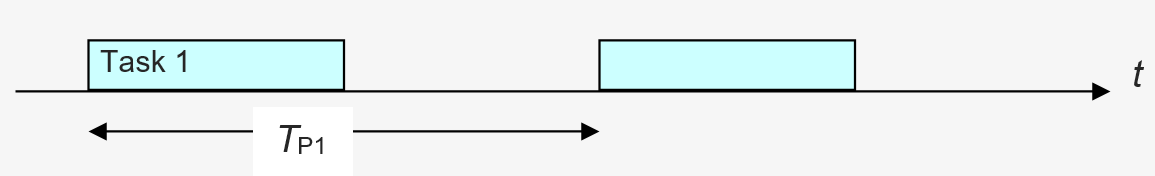
\includegraphics[width=10cm, height=2cm]{Images/image83.png}
    %\caption{}
    \label{fig:Fig 29}
    \end{figure}
\newpage
A second periodic task with a period of \textit{T}${}_{P2}$ = 100 ms and an execution time of \textit{T}${}_{e2}$ = 50 ms also causes a processor demand of \textit{H}${}_{2}$ = 50 \%.

	\begin{figure}[h]
    \centering
    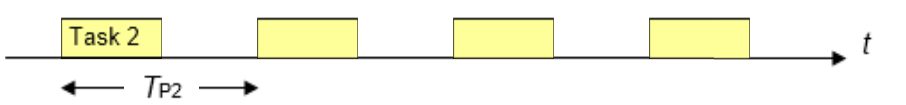
\includegraphics[width=10cm, height=2cm]{Images/image84.png}
    %\caption{}
    \label{fig:Fig 30}
    \end{figure} 

An implicit timing condition for each periodic task is: task execution must be finished before the next period starts (deadline) !\\

Both tasks cause a total processor demand \textit{H} = \textit{H}${}_{1}$ + \textit{H}${}_{2}$ = 100~\%.

	\begin{figure}[h]
    \centering
    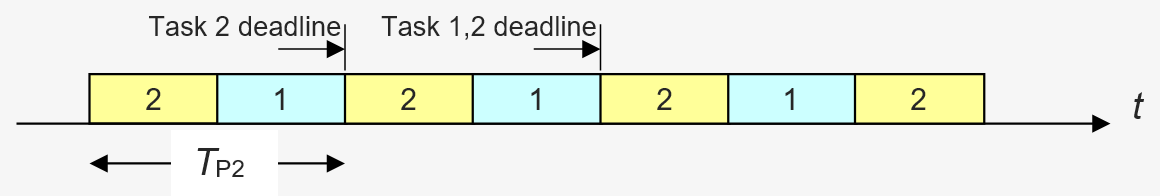
\includegraphics[width=10cm, height=3cm]{Images/image85.png}
    %\caption{}
    \label{fig:Fig 31}
    \end{figure} 
    
One possible schedule for executing both tasks is to displace task 1 after exactly half of its execution time by task 2, which is never displaced. Thus, task 1 must be displaceable:

	\begin{figure}[h]
    \centering
    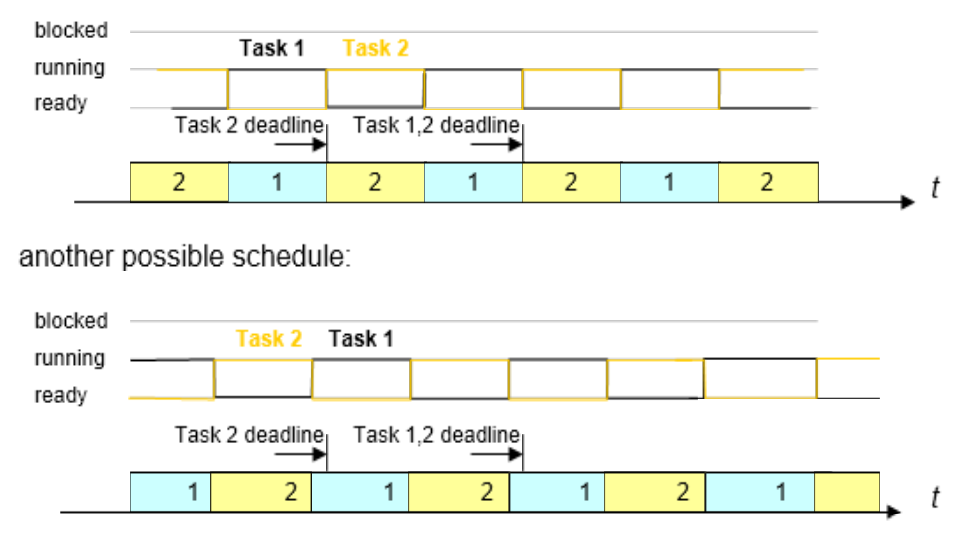
\includegraphics[width=12cm, height=8cm]{Images/image86.png}
    %\caption{}
    \label{fig:Fig 32}
    \end{figure} 

In general, for a tasklet of \textit{n} periodic tasks, the total processor demand

\begin{equation}
	H=\sum _{i=1}^{n}\frac{T_{ei} }{T_{pi}}
\label{EQ 3}
\end{equation}

$T_{ei}$ execution time of task i, $T_{pi}$ periodic time of task i\\
\newpage

{\rot\bf Classification of Scheduling Algorithms}

	\begin{figure}[h]
    \centering
    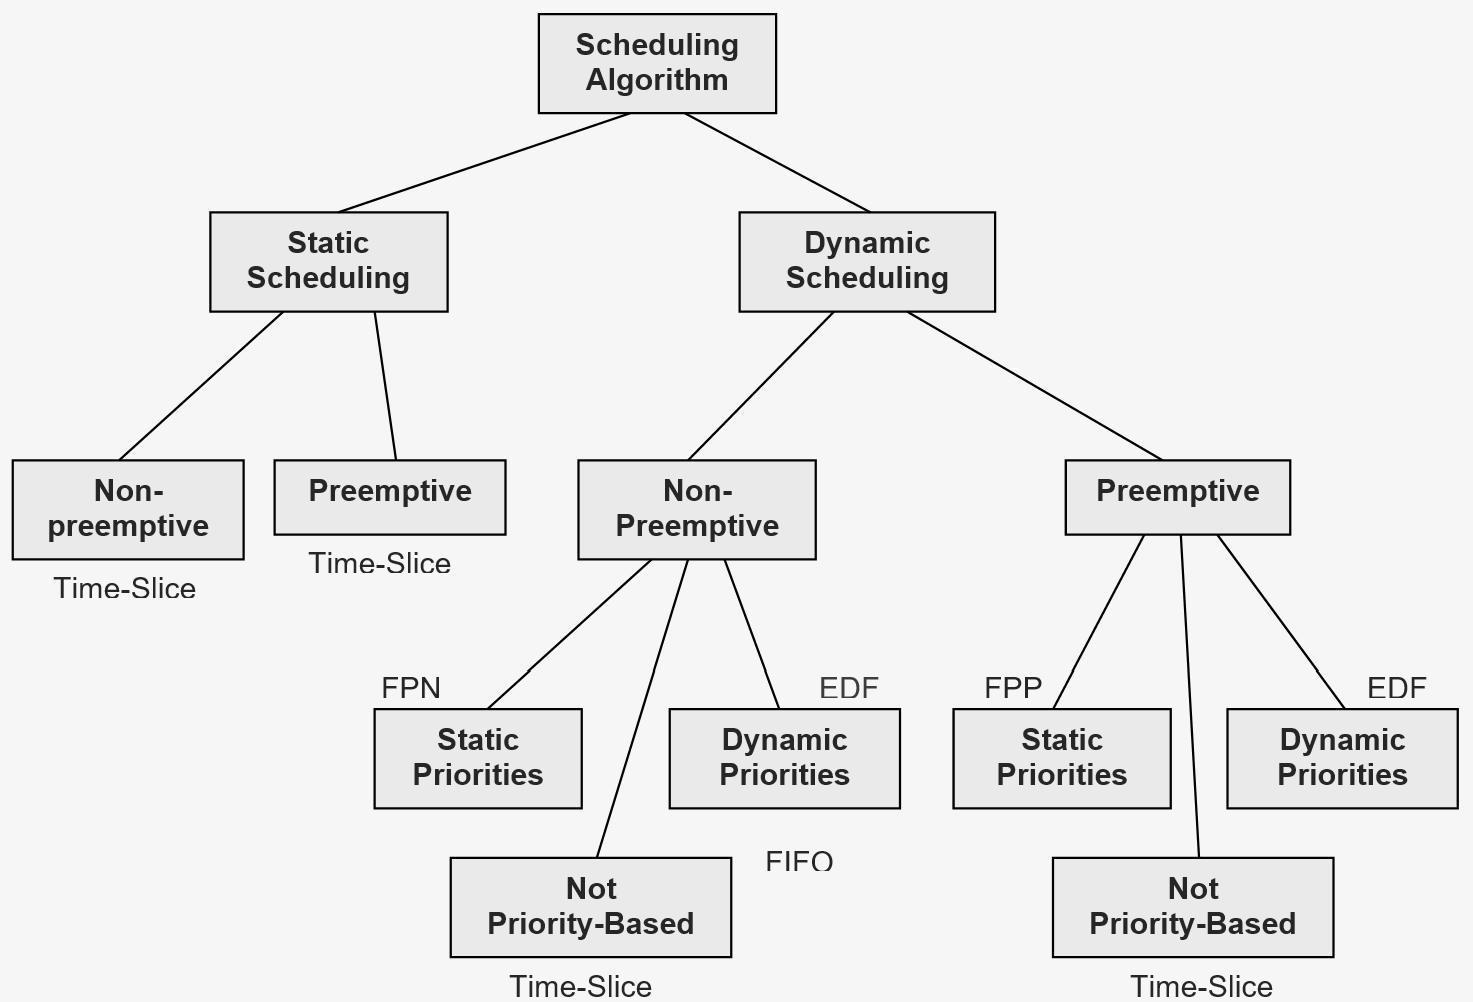
\includegraphics[width=15cm, height=10cm]{Images/image88.png}
    %\caption{}
    \label{fig:Fig 33}
    \end{figure}
    
{\rot\bf Static Scheduling}\\

Prior to the execution of a taskset an allocation table (dispatching table) with the start times exists, regarding time constraints and dependencies of each task. The dispatcher as part of the RTOS kernel assigns the individual tasks due to this table 

$\rightarrow$ principle of synchronous programming.\\

\textbf{Advantage: }  minimal overhead, as no decisions are needed at runtime. \\

\textbf{Disadvantage: }  restriction to periodic events.\\

{\rot\bf Dynamic Scheduling}\\

Here for the execution of tasks different criteria are used by the dispatcher \textbf{at runtime}, taking into account start times, time conditions (deadlines), and dependencies of each task. Asynchronous programming. Advantage  increased flexibility and the opportunity to respond to aperiodic events. Disadvantage  increased overhead, lower predictability\\

{\rot\bf Static and Dynamic Priorities}\\

(Not to be confused with static/dynamic scheduling). The scheduler can use priorities for the allocation of resources (processor, memory, I/O,{\dots}) to a task. \textbf{Static priorities} are set before running the application and are never changed during runtime. \textbf{Dynamic priorities} can be adjusted for each task \textbf{at runtime}. Furthermore, there are algorithms, using \textbf{No Priorities} at all. 

\subsection{Preemption}

(= "Prioritization") is an important feature for a scheduler, which describes the capability for displacing a running task for later execution in favor of another task. 

\textbf{Preemptive scheduling }means that a less important task can be displaced by a more important task. The most important task with \textbf{\textit{ready}}-state will be executed immediately. The less important task will be continued again until no other more important task waits with \textbf{\textit{ready}}-state.

	\begin{figure}[h]
    \centering
    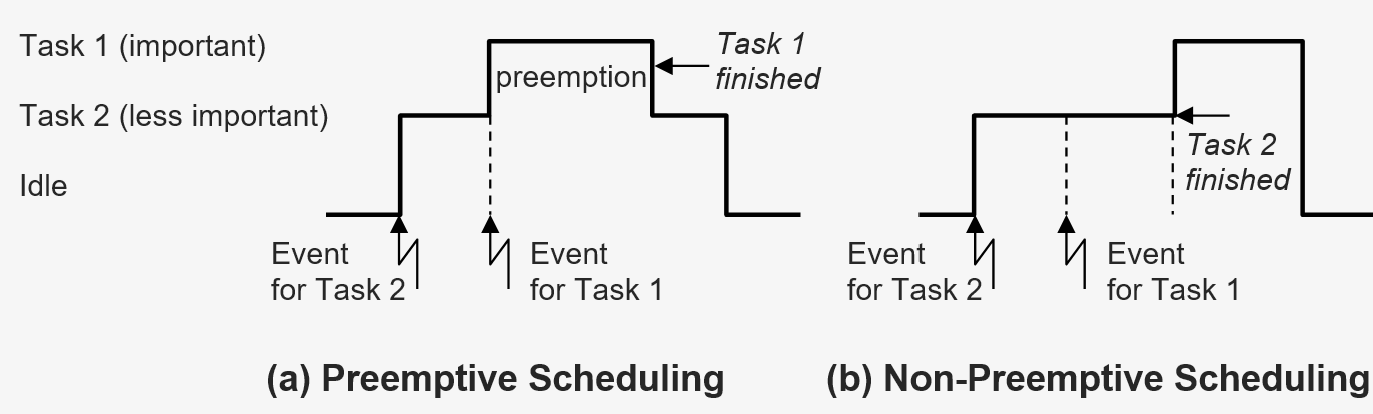
\includegraphics[width=14cm, height=4cm]{Images/image89.png}
    %\caption{}
    \label{fig:Fig 34}
    \end{figure}

\textbf{Non-preemptive scheduling} (= \textbf{cooperative scheduling}) means, that there is no displacement of a running task. Only after the current task is finished or blocked, the next task with \textbf{\textit{ready}} state is executed.\\


{\rot\bf Time-Slice Scheduling (Round-Robin Scheduling)}\\

Time-Slice Scheduling (time slicing) assigns each task a fixed time slice (Time Slice). The order of task execution corresponds to the sequence of \textbf{\textit{ready}}-tasks entering the task-list of the OS scheduler (FIFO principle). The duration of the time slice for a task can be set individually.\\

This type of time-slice scheduling is a dynamic preemptive scheduling. 

\begin{itemize}
	\item TSS does not use priorities
	\item time slot duration can be chosen individually for each task
	\item With time slices chosen fine-grained enough TSS is approaching optimality.
\end{itemize}

	\begin{figure}[h]
    \centering
    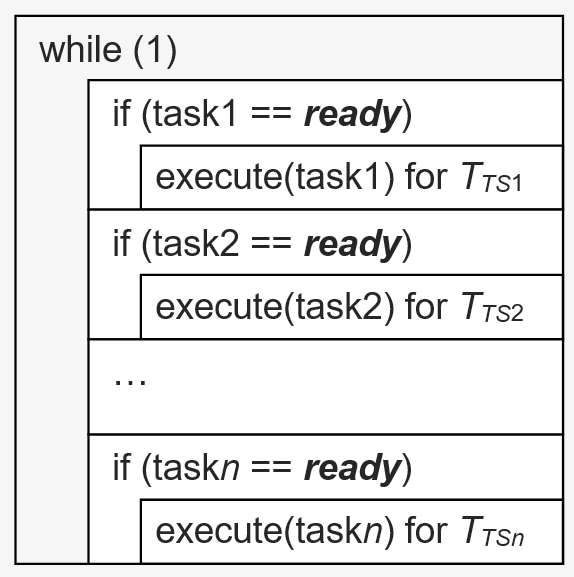
\includegraphics[width=6cm, height=5cm]{Images/image90.png}
    %\caption{}
    \label{fig:Fig 35}
    \end{figure}
\newpage
\textbf{Principle of Time-Slice (Round-Robin) Scheduling: }

\begin{tcolorbox}[colback=blue!5!white,colframe=blue!75!black]
  All \textbf{\textit{ready}}-tasks are queued in a FIFO \\
  Each task \textit{i} gets assigned a time slice (time slice, quantum) \textit{T${}_{TSi}$}
  \begin{itemize}
		\item  the task is preempted, i.e. displaced to the \textbf{\textit{ready}} state
		\item  the task is put at the end of the FIFO queue;
		\item  The first task in the FIFO will be executed.
	\end{itemize}
  
  If a task changes state from \textbf{\textit{blocked}} to \textbf{\textit{ready}}, it will be put at the end of the FIFO queue
\end{tcolorbox}

Typical Applications: \textbf{Kernel-mode programs} \\ 

Example 1: 3 Tasks with $H_{max}$ $<$ 0.778, from \textbf{[wörnB]}, same as in section 2.2.7:\\
Task T1: period \textit{T}${}_{p1}$ = 10~ms, execution time \textit{T}${}_{e1}$ = 1~ms $\rightarrow$ \textit{H}${}_{1}$ = 0.1\\
Task T2: period \textit{T}${}_{p2}$ = 10~ms, execution time\textit{ T}${}_{e2}$ = 5~ms $\rightarrow$ \textit{H}${}_{2}$ = 0.5\\
Task T3: non-periodic, period \textit{T}${}_{p3}$ = deadline \textit{T}${}_{d3}$ = 15.4~ms, \textit{T}${}_{e3}$ = 2.62~ms $\rightarrow$ \textit{H}${}_{3}$ = 0.17\\


By (2.2) the total CPU utilization \textit{H} = 0.1 + 0.5 + 0.17 = 0.77 \\

One chooses a basic time-slice \textit{T}${}_{TS}$ = 1 ms and assigns individual time slices as multiples of \textit{T}${}_{TS}$ with $\Sigma$\textit{T}${}_{TS}$ = 9 ms:\\

Task T1:    \textit{T}${}_{TS1}$ = 1 $.$\textit{T}${}_{TS}$ = 1 ms $\rightarrow$ \textit{H}${}_{1}$ = \textit{T}${}_{TS1}$/$\Sigma$\textit{T}${}_{TS}$ = 1~ms / 9~ms = 11~\%\\
Task T2:    \textit{T}${}_{TS2}$ = 5 $.$\textit{T}${}_{TS}$ = 5 ms $\rightarrow$ \textit{H}${}_{2}$ = \textit{T}${}_{TS2}$/$\Sigma$\textit{T}${}_{TS}$ = 5~ms / 9~ms = 55~\%\\
Task T3:     \textit{T}${}_{TS3}$ = 3 $.$\textit{T}${}_{TS}$ = 3 ms $\rightarrow$ \textit{H}${}_{3}$ = \textit{T}${}_{TS3}$/$\Sigma$\textit{T}${}_{TS}$ = 3~ms / 9~ms = 33~\%

	\begin{figure}[h]
    \centering
    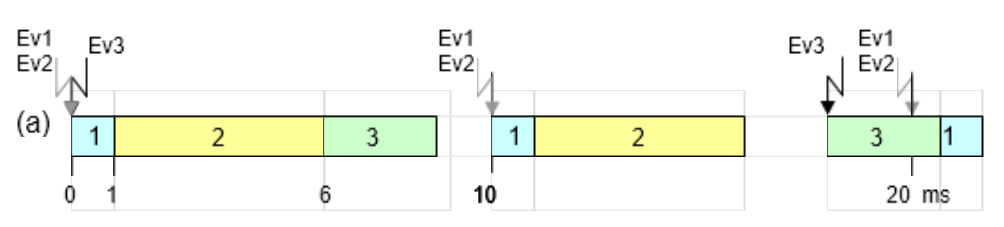
\includegraphics[width=13cm, height=3cm]{Images/image91.png}
    %\caption{}
    \label{fig:Fig 36}
    \end{figure}

In this example the assigned time slices were chosen to be larger than the execution times of each task, in order to avoid preemption.\\

With TSS a context-switch can occur at the end of a time-slice only. which can cause some \textit{jitter} (as with task T1 above).\\

{\rot\bf Fixed Time-Slice-Scheduling }\\

FT scheduling is based on a TDMA approach, requires no priorities, and is therefore frequently used in embedded microcontroller applications without an operating system.\\

A strictly periodic schedule is created with a periodic time \textit{N·T${}_{TS}$}, i.e. with \textit{N} integer multiples of the basic \textit{T${}_{TS}$} time slice. Each task gets assigned one (ore more) basic time slots, large enough to hold the WCET of each:\\

	\begin{figure}[h]
    \centering
    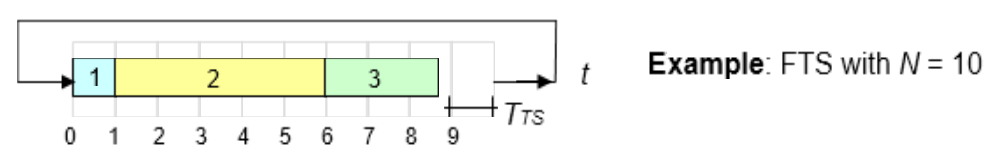
\includegraphics[width=12cm, height=2cm]{Images/image92.png}
    %\caption{}
    \label{fig:Fig 37}
    \end{figure}

Conditions for Events are polled within each task, if a task is not finished at the end of its timeslice, it can be preempted (\textbf{\textit{preemptive FTS}})or not (\textbf{\textit{cooperative FTS}}).\\

The previous example with three tasks, and an idle task T4 at a period \textit{N}$\mathrm{\bullet}$\textit{T${}_{TS}$} = $\Sigma$\textit{T${}_{TS}$} = 10 ms is realized, the time slices are chosen as multiples of \textit{T${}_{TS}$} = 1 ms as follows \\

Task T1:    \textit{T${}_{TS}$}${}_{1}$ = 1 $.$\textit{T${}_{TS}$} = 1 ms $\rightarrow$ \textit{H}${}_{1}$ = \textit{T${}_{TS}$}${}_{1}$/$\Sigma$\textit{T${}_{TS}$} = 1~ms / 10~ms = 10~\%

Task T2:    \textit{T${}_{TS}$}${}_{2}$ = 5 $.$\textit{T${}_{TS}$} = 5 ms $\rightarrow$ \textit{H}${}_{2}$ = \textit{T${}_{TS}$}${}_{2}$/$\Sigma$\textit{T${}_{TS}$} = 5~ms / 10~ms = 50~\%

Task T3:     \textit{T${}_{TS}$}${}_{3}$ = 3 $.$\textit{T${}_{TS}$} = 3 ms $\rightarrow$ \textit{H}${}_{3}$ = \textit{T${}_{TS}$}${}_{3}$/2$\Sigma$\textit{T${}_{TS}$} = 3~ms / 10~ms = 30~\%

Task T4 (idle) \textit{T${}_{TS}$}${}_{4}$ = 1 $.$\textit{T${}_{TS}$} = 1 ms $\rightarrow$ \textit{H}${}_{4}$ = 10~\%

	\begin{figure}[h]
    \centering
    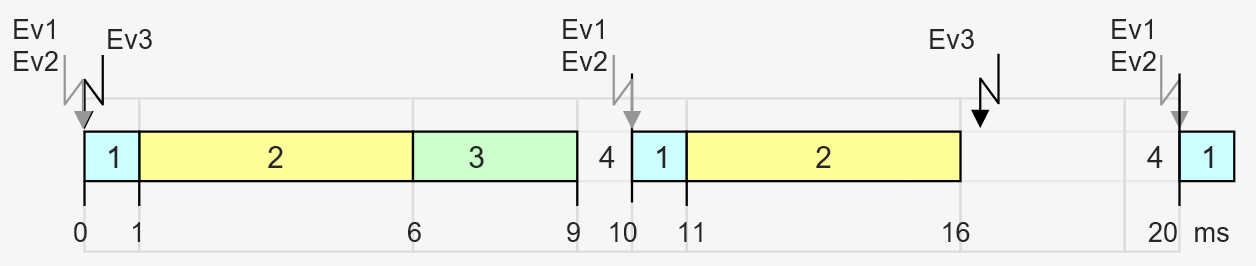
\includegraphics[width=13cm, height=3cm]{Images/image93.png}
    %\caption{}
    \label{fig:Fig 38}
    \end{figure}

T3 runs for the second time at \textit{t} = 26 ms the delay of 10 ms does not result in a T3-deadline violation. The idle task T4 provides a placeholder for unused CPU load, which can be used in modern CPUs for power saving features.\\

\textbf{Advantage of fixed TSS}: the execution times can be defined exactly!\\

{\rot\bf Binary Fixed Time-Slice-Scheduling }\\

If task periodic times \textit{T${}_{Pi}$} can be represented as power-of-2 integer multiples of a basic time slice \textit{T${}_{TS}$}, one can obtain a periodic binary schedule:\\

	\begin{figure}[h]
    \centering
    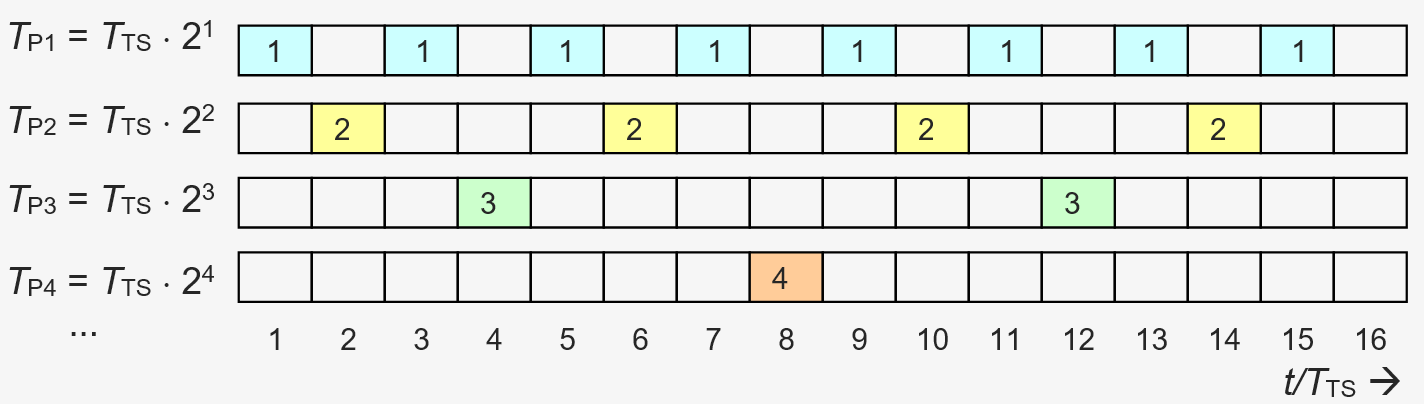
\includegraphics[width=12cm, height=3.5cm]{Images/image94.png}
    %\caption{}
    \label{fig:Fig 39}
    \end{figure}

If the maximum time of execution is \textit{T}${}_{TS}$ and equal for each task, the utilization for each task is 

\begin{equation}
	 H_{i} =\frac{T_{ei} }{T_{pi} } =\frac{T_{TS} }{2^{i} \cdot T_{TS} } =2^{-i} \hspace{3cm} \sum_{i=1}^N H_{i} \stackrel{N\to \infty }{\longrightarrow} 1
\label{EQ }
\end{equation}

Thus, the fastest task with periodic time \textit{T${}_{p}$}${}_{1}$ = 2$.$\textit{T}${}_{TS}$ is assigned 50~\% of the complete processing time, task 2 with periodic time \textit{T${}_{p}$}${}_{2}$ = 4$.$\textit{T}${}_{TS}$ gets assigned 25~\%, task 3 gets 12.5~\%, {\dots}\\

From (2.3) it shows, that the total utilization of \textit{H} aiming with an infinite number of tasks to 100\%, thus, there will be no overload situations, if all tasks meet their maximum execution time \textit{T${}_{TS}$} requirement (easily guaranteed with a preemptive schedule).\\

\textit{   T${}_{TS}$} $\mathrm{\ge}$ max(\textit{T${}_{e}$}${}_{1}$,\textit{ T${}_{e}$}${}_{2}$,\textit{ T${}_{e}$}${}_{3}$, ..)\\

With a non-preemptive schedule (cooperative task schedule) maximum execution times \textit{T${}_{ei}$} have to be determined carefully (WCET determination), such, that each task can complete execution within the basic \textit{T${}_{TS}$}. If a task gets delayed for some reasons (like high priority interrupts during execution) the complete schedule will get delayed.\\

\textbf{Advantages }\\

Binary fixed time-slice scheduling is

\begin{itemize}
	\item  quite suitable with multirate sampling systems (e.g. oversampling, when integer multiples of a common sampling frequency are needed).
	\item  a very simple scheduling without priorities,
	\item  suitable in a non-preemptive realization for even small microcontrollers without OS. 
	\item  Time and duration of execution for each task is guaranteed (apart from interrupts)
\end{itemize}

\textbf{Disadvantages }

\begin{itemize}
	\item \textbf{ }Binary time-slice scheduling is not fully flexible with arbitrary periodic times and execution times
	\item  can turn into very complex software, especially with integrating tasks with execution time larger than \textit{T${}_{TS}$}.
\end{itemize}

\textbf{Lab-Experiment}   \textbf{\underbar{AVR-Timer-Interrupts-(FTS-Scheduling)}}

	\begin{figure}[h]
    \centering
    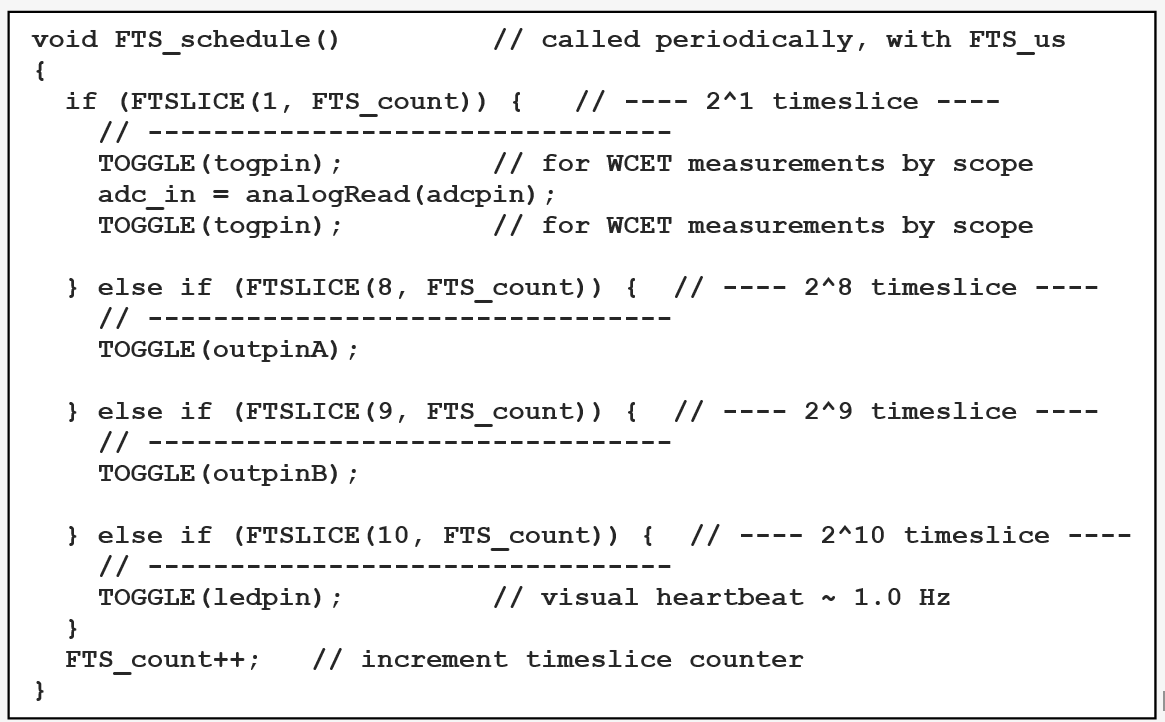
\includegraphics[width=13cm, height=7cm]{Images/image95.png}
    %\caption{}
    \label{fig:Fig 40}
    \end{figure}

\textbf{\underbar{Sketch for Arduino Nano}  (FixedTimeSlice.ino)}\\
\newpage
\textbf{Example}: 4 periodic tasks (on an AVR µC, from section Digital PID Control with 4 Tasks) \\

\textit{T${}_{p}$}${}_{1}$ = \textit{T${}_{p}$}${}_{2}$ = 1 ms, \textit{T${}_{p}$}${}_{3}$ = 16 ms, \textit{T${}_{p}$}${}_{4}$ = 8 ms

\textit{T${}_{e}$}${}_{1}$ = 50 µs, \textit{T${}_{e}$}${}_{2}$ = 0.3 ms, \textit{T${}_{p}$}${}_{3}$ = 40 µs, \textit{T${}_{p}$}${}_{4}$ = 40 µs

\textit{H}${}_{1}$ = 5 \%, \textit{H}${}_{2}$ = 30 \%, \textit{H}${}_{3}$ = 0.1/20 = 0.5 \%, $\rightarrow$ \textit{H}${}_{4}$ = 0.05/20 = 0.25 \%  \textit{H} = 30.75 \%\\

Solution with Binary time-slice schedule with 3 Tasks, \textit{T${}_{TS}$} = 0.5 ms, \textit{T${}_{TS}$} $\mathrm{\ge}$ max(\textit{T${}_{ei}$}) = max(0.3, 0.05, 0.005 0.0025 ms) tasks with the same periodic times run in the same time-slice:\\
 $\rightarrow$ T1 und T2 executed successively in the 2 Timeslice 2·\textit{T${}_{TS}$ }= 1 ms\\
 
 
 	\begin{figure}[h]
    \centering
    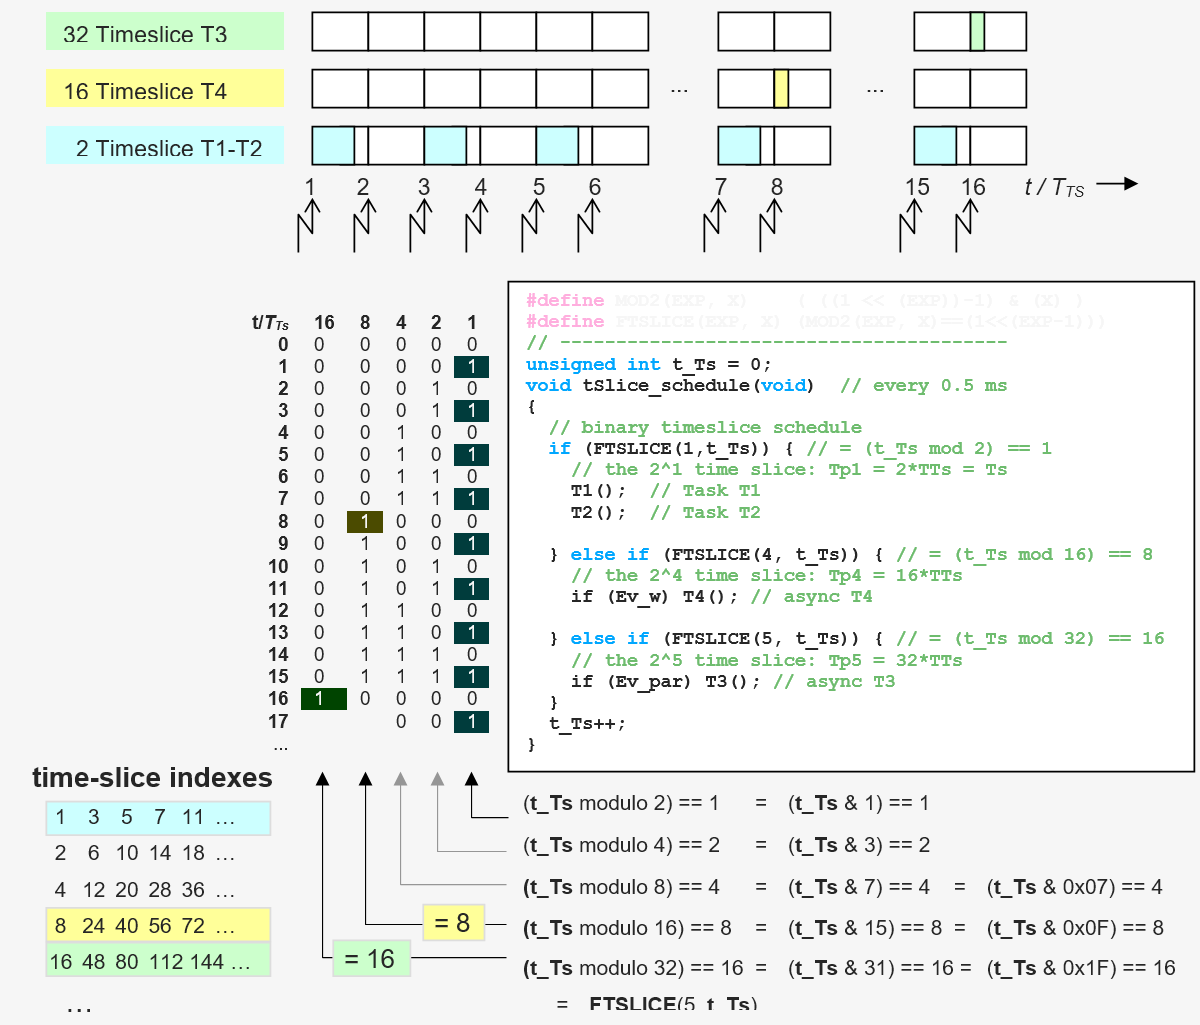
\includegraphics[width=15cm, height=11cm]{Images/image96.png}
    %\caption{}
    \label{fig:Fig 41}
    \end{figure}

\textbf{Proof for collision-free assignment of time-slice indexes } (with \textit{k},\textit{l} $\in$ \textbf{$\boldsymbol{\mathbb{Z}}$}  integers)\\

for some period \textit{N} we get time slices at indexes  \textit{n${}_{k}$}  =  \textit{k$\bullet$N  +  $\frac{N}{2} $}  e.g.: 2, 6, 10, 14, ..\\

thus, for period 2\textit{N} (next time slice) we get    \textit{m${}_{l}$} =  \textit{l$\bullet$}2\textit{N  +  N  }e.g.: 4, 12, 20, 28, ..\\

for a collision, we set \textit{n${}_{k}$} ${\mathop{=}\limits^{!}} $ \textit{m${}_{l}$}. Division by \textit{N} on both sides shows \textit{k} + 0.5 ${\mathop{=}\limits^{!}} $ 2$\mathrm{\bullet}$\textit{l} + 1, which has no solution with integers \textit{k} and \textit{l}, thus the above assignment is without any conflict all time slice indexes (proof by full induction) !
\newpage

\subsection{FIFO Scheduling}

The name derives from the FIFO (first in, first out) principle of a waiting queue:    

 	\begin{figure}[h]
    \centering
    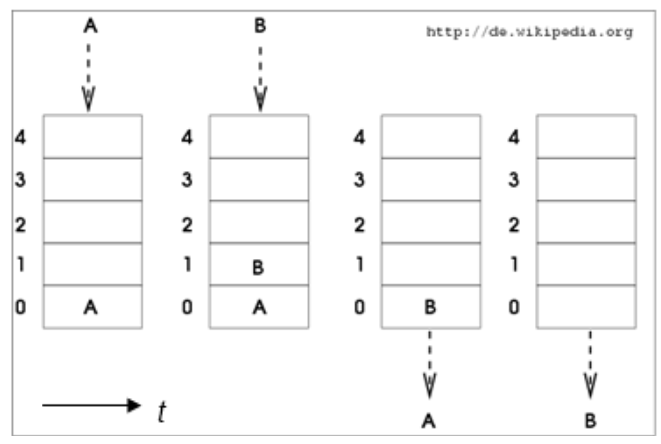
\includegraphics[width=10cm, height=5cm]{Images/image97.png}
    %\caption{}
    \label{fig:Fig 42}
    \end{figure}

where elements put into a queue in a certain order of sequence, are taken out in the same order of sequence.With a \textbf{FIFO scheduler}, the tasks are processed in the same order in which they have taken the ready state.  

$\rightarrow$ An running task is not interrupted, it is a \textbf{non-preemptive}, \textbf{dynamic} scheduler.\\

Advantage:   very simple implementation, sometimes used in universal OS\\

Disadvantage:  bad real-time performance,        violations of time conditions even at low processing demands ( example)\\

\textbf{Example}: Two tasks with FIFO scheduling\\

Task 1: \textit{T}${}_{p1}$ = 150 ms, \textit{T}${}_{e1}$ = 15 ms   \textit{H}${}_{1}$ = 0.1

Task 2: \textit{T}${}_{p2}$ = 10 ms,  \textit{T}${}_{e2}$ = 1 ms    \textit{H}${}_{2}$ = 0.1\\

For both periodic tasks there is a time bound (deadline) with the next period. With (2.2) \\

\textit{H} = \textit{H}${}_{1}$ + \textit{H}${}_{2}$ = 0.1 + 0.1 = 0.2 

For 20 \% processor demand only, it should be easy to find a schedule for this taskset, but:

 	\begin{figure}[h]
    \centering
    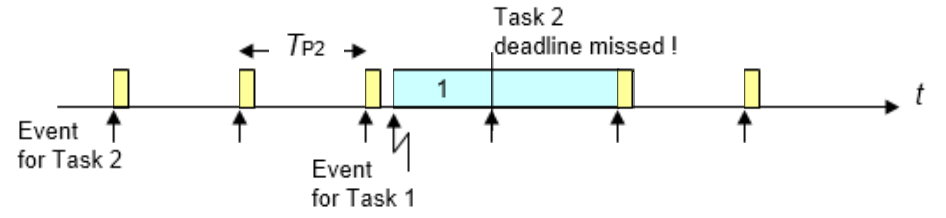
\includegraphics[width=12cm, height=2.5cm]{Images/image98.png}
    %\caption{}
    \label{fig:Fig 43}
    \end{figure}

This simple example shows that even at a very low processor demand, a FIFO scheduler \textbf{cannot} \textbf{guarantee} compliance with the real-time conditions.\\

{\rot\bf Fixed-Priority Scheduling}\\

For fixed-priority scheduling, each task is assigned a fixed priority. The \textbf{\textit{ready}}-task with the highest priority waiting in the scheduler's queue is assigned to the processor.  \\
$\rightarrow$ fixed-priority scheduling is\textbf{ dynamic scheduling with static priorities}. (often used with interrupt processing of microprocessors, preemptive or non-preemptive):

\begin{enumerate}
	\item  \textbf{Fixed-Priority-Preemptive Scheduling (FPP)}\\
	If a \textbf{task with higher priority} than the currently running gets into the ready state, then the \textbf{current task is interrupted (displaced, preemted)} and the task with the higher priority is assigned to the processor immediately.
	
	\item  \textbf{Fixed-Priority-Non-Preemptive Scheduling (FPN)}\\
	If a \textbf{task with higher priority} than the currently running gets into the ready state, then the \textbf{task is assigned} to the processor only \textbf{after the current task} is either \textbf{completed} or \textbf{blocked}.
\end{enumerate}

\textbf{Advantage}: with FPP, the compliance with the real-time conditions can be guaranteed (unlike to FIFO scheduling), if the priorities were assigned appropriate. \\

The assignment of priorities to tasks is an important step in the development of a real-time application.\\

{\rot\bf Rate-Monotonic-Scheduling (RMS)}\\

For purely periodic applications, there is a rule, the so-called \textbf{rate-monotonic scheduling rule}, which states, that the priority of the tasks to be performed is inversely proportional to their periodic time:

\begin{equation}
	PR_{i} \sim \frac{1}{T_{pi} } 
\label{EQ }
\end{equation}

$PR_i$ Priority task i, $T_{pi}$ Periodic time of task i\\

under the (rather idealized) conditions:

\begin{itemize}
	\item  Preemptive scheduling is used
	\item  The periodic times \textit{T${}_{Pi}$} are constant 		
	\item  The time limits (deadlines) are equal to the periodic times \textit{T${}_{Pi}$}
	\item  The execution times are known and constant \textit{T${}_{ei}$}
	\item  The tasks are independent from each other (can not deadlock)
\end{itemize}

\textbf{Example}: (same as with FIFO scheduling in section 2.2.6). Two tasks with Fixed-Priority-Preemptive Scheduling (FPP):\\

Task 1: \textit{T}${}_{p1}$ = 150 ms, \textit{T}${}_{e1}$ = 15 ms,   lower priority by   (2.4)\\
Task 2: \textit{T}${}_{p2}$ = 10 ms,  \textit{T}${}_{e2}$ = 1 ms   higher priority by (2.4)\\

 	\begin{figure}[h]
    \centering
    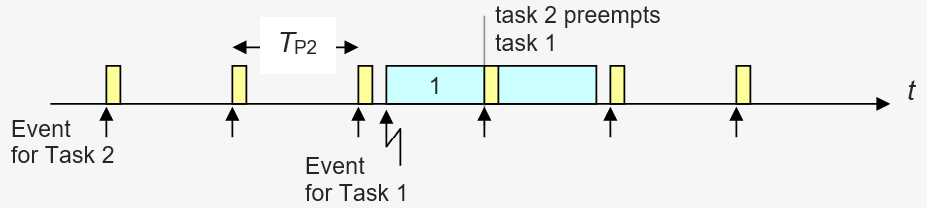
\includegraphics[width=12cm, height=2.5cm]{Images/image99.png}
    %\caption{}
    \label{fig:Fig 44}
    \end{figure}

The running task 1 is displaced with an event for task 2, which has higher priority (its state goes from \textbf{\textit{blocked}}  \textbf{\textit{ready}}), so that the deadline of task 2 is not violated (in contrast to FIFO scheduling).\\

Obviously,\textbf{ FPP scheduling} with \textbf{RMS} provides much better results than FIFO scheduling. \\

In contrast, with \textbf{FPN}, the deadlines of task 2 would be violated !\\

In general

\begin{tcolorbox}[colback=blue!5!white,colframe=blue!75!black]
 	With periodic tasks with fixed priorities and deadlines equal to their periodic times, rate-monotonic scheduling (RMS) provides for an optimal priority allocation.
\end{tcolorbox}

This also means that FPP scheduling with RMS always delivers an executable schedule, if one exists. However, the overall CPU utilization may not exceed \textit{H${}_{max}$ }([1], by Liu)\\

\begin{equation}
	H_{\max } =n\cdot \left(2^{1/n} -1\right)=n\cdot \left(\sqrt[{n}]{2} -1\right) 
\label{EQ }
\end{equation}

$n$ number of tasks\\

\begin{table}[h!]
\setlength{\tabcolsep}{10pt} % Default value: 6pt
\renewcommand{\arraystretch}{1.5} % Default value: 1
\small
\centering
 \begin{tabular}{|c|c|c|c|} 
 \hline
 \textbf{n} & \textbf{$H_{max}$} \\ [0.1ex] \hline
1 & 1.000000 \\ \hline
2 & 0.828427 \\ \hline
3 & 0.779763 \\  \hline
4 & 0.756828 \\ \hline
5 & 0.743492 \\ \hline
10 & 0.717735 \\ \hline 
20 & 0.705298 \\ \hline 
50 & 0.697974 \\ \hline 
100 & 0.695555 \\ \hline 
1000 & 0.693387 \\ \hline 
10000 & 0.693171 \\ \hline 
 \end{tabular}
 %\caption{\textbf{}}
 \label{}
\end{table}

The limit (2.5) can be used to examine the feasibility of a (periodic) taskset and to guarantee the conformance with all time limits.FPP with RMS is very popular because of its simplicity. \\

However, there are problems at very high utilization (beyond or near \textit{H${}_{max}$}) and with RMS at the same or nearly the same time periods, delivering same task priorities. Furthermore, there are sometimes difficulties in approaching non-periodic processes by periodic processes with sufficient precision.\\

\textbf{Example 1:} 3 Tasks with \textit{H}${}_{max}$ $\mathrm{>}$ 0.778, from [W\"{o}rnB] : \\
Task T1: period \textit{T}${}_{p1}$ = 10~ms, execution time \textit{T}${}_{e1}$ = 1~ms $\rightarrow$ \textit{H}${}_{1}$ = 0.1\\
Task T2: period \textit{T}${}_{p2}$ = 10~ms, execution time\textit{ T}${}_{e2}$ = 5~ms $\rightarrow$ \textit{H}${}_{2}$ = 0.5\\
Task T3: non-periodic, deadline = \textit{T}${}_{d3}$ = 15.4~ms, execution time\textit{ T}${}_{e3}$ = 5.5~ms\\

By (2.2) the total CPU utilization \textit{H} = 0.1 + 0.5 + 0.357 = 0.957, amost 100 \% !But with (2.5) \textit{H} $\mathrm{>}$ \textit{H}${}_{max}$ $\mathrm{>}$ 0.78 deadlines will be violated with \textbf{FPP/RMS} with 3 tasks.\\ 

FPP/RMS \textbf{can't deliver an executable schedule}, as this example shows:\\

By (2.4) one has 2 choices for assigning the priorities due to the equal periods \textit{T}${}_{p1}$\textit{ }and \textit{T}${}_{p2}$:\\

\begin{table}[h!]
\setlength{\tabcolsep}{10pt} % Default value: 6pt
\renewcommand{\arraystretch}{1.5} % Default value: 1
\small
\centering
 \begin{tabular}{|c|c|c|c|} 
 \hline
 \textbf{Priority assignment (a)} & \textbf{Priority assignment (b)} \\ [0.1ex] 
 \hline
 T1  high priority & T2  high  priority \\ 
 \hline
 T2  medium priority & T1  medium priority \\ 
  \hline
 T3  low priority & T3  low priority  \\ 
 \hline
 \end{tabular}
 %\caption{\textbf{}}
 %\label{Intrinsic}
\end{table}

In both cases there is a violation of the T3 deadline, if all tasks get \textbf{\textit{ready}} the same time at \textit{t} = 0: 

 	\begin{figure}[h]
    \centering
    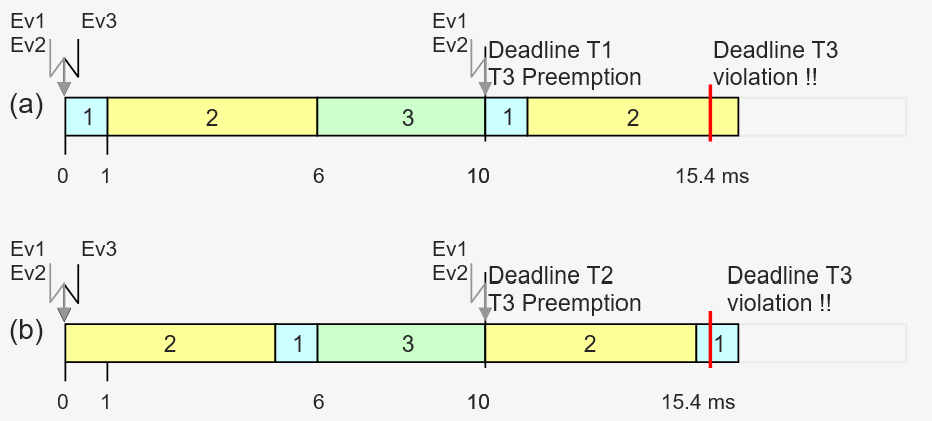
\includegraphics[width=12cm, height=5cm]{Images/image100.png}
    %\caption{}
    \label{fig:Fig 45}
    \end{figure}
    
Of course, the violation of T3 deadline in the example above occurs due to the deliberate disregard of the load limit \textit{H${}_{max}$}, by \eqref{GrindEQ__2_5_}. If one meets the max. load requirement \textit{H} $\mathrm{<}$ 78\% (n = 3), there is violation of the T3 deadline.\\

However, with growing number of tasks the maximum load goes down as low as 70\% (from n $\mathrm{>}$ 10), which is surprisingly low.\\

Ideas to achieve higher processor loads lead to dynamic assignment of priorities.\\

 \textbf{Example 2:} 3 Tasks with \textit{H}${}_{max}$ $\mathrm{<}$ 0.778, from [W\"{o}rnB] :\\
Task T1: period \textit{T}${}_{p1}$ = 10~ms, execution time \textit{T}${}_{e1}$ = 1~ms  $\rightarrow$ \textit{H}${}_{1}$ = 0.1\\
Task T2: period \textit{T}${}_{p2}$ = 10~ms, execution time\textit{ T}${}_{e2}$ = 5~ms  $\rightarrow$ \textit{H}${}_{2}$ = 0.5\\
Task T3: non-periodic, period \textit{T}${}_{p3}$ = deadline \textit{T}${}_{d3}$ = 15.4~ms, \textit{T}${}_{e3}$ = 2.62~ms  $\rightarrow$ \textit{H}${}_{3}$ = 0.17\\

By (2.2) the total CPU utilization \textit{H} = 0.1 + 0.5 + 0.17 = 0.77 With (2.5) \textit{H} $\mathrm{<}$ \textit{H}${}_{max}$ = 0.78 deadlines will be not violated with FPP/RMS with 3 tasks:\\

By (2.4) one has 2 choices for assigning the priorities due to the equal periods \textit{T}${}_{p1}$\textit{ }and \textit{T}${}_{p2}$:

\begin{table}[h!]
\setlength{\tabcolsep}{10pt} % Default value: 6pt
\renewcommand{\arraystretch}{1.5} % Default value: 1
\small
\centering
 \begin{tabular}{|c|c|c|c|} 
 \hline
 \textbf{Priority assignment (a)} & \textbf{Priority assignment (b)} \\ [0.1ex] 
 \hline
 T1  high priority & T2  high  priority \\ 
 \hline
 T2  medium priority & T1  medium priority \\ 
  \hline
 T3  low priority & T3  low priority  \\ 
 \hline
 \end{tabular}
 %\caption{\textbf{}}
 %\label{Intrinsic}
\end{table}

In both cases there is no violation of the T3 deadline, even if all tasks get \textbf{\textit{ready}} the same time at \textit{t} = 0: 
	
	\begin{figure}[h]
    \centering
    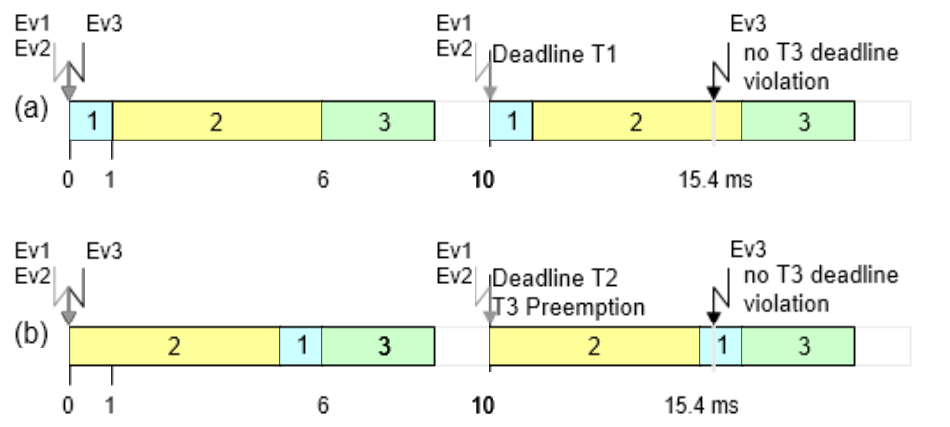
\includegraphics[width=12cm, height=5cm]{Images/image187.png}
    %\caption{}
    \label{fig:Fig 46}
    \end{figure}
\newpage   
$\rightarrow$ If one meets the max. load requirement \textit{H} $\mathrm{<}$ 78\% (n = 3), there is violation of the T3 deadline.\\

However, with 3 tasks the maximum load allowed is as low as 77.8\% (for \textit{n} = 3), which is surprisingly low.\\

Ideas to achieve higher processor loads lead to dynamic assignment of priorities \\
$\rightarrow$ next sections.\\

{\rot\bf Earliest-Deadline-First Scheduling (EDF)}\\

In Earliest-Deadline-First Scheduling (EDF) the Task Processor is granted to that \textbf{\textit{ready}}-task, which is closest to its time limit (deadline). This is achieved by assigning the task priorities according to the vicinity to the individual deadlines.\\

$\rightarrow$ EDF is dynamic scheduling with dynamic priorities, either preemptive or non-preemptive\\

For \textbf{preemptive EDF scheduling} a context-switch is made, when a task with earlier time bound gets \textbf{\textit{ready}}. In \textbf{non-preemptive EDF scheduling} is the task with the shortest time interval ist executed only, if the currently running task is finished or blocked.\\

Preemptive EDF scheduling, is used more frequently than non-preemptive EDF scheduling, which is essentially only used when non-interruptible processes are to be managed, such as disk access.\\

\textbf{Advantage}: With \textbf{preemptive EDF scheduling }100 \% CPU utilization can be achieved. \\

\textbf{Example} with 3 Tasks (same as in section 2.2.7): Task T1: period \textit{T}${}_{p1}$ = 10~ms, execution time \textit{T}${}_{e1}$ = 1~ms  \textit{H}${}_{1}$ = 0.1Task T2: period \textit{T}${}_{p2}$ = 10~ms, execution time\textit{ T}${}_{e2}$ = 5~ms  \textit{H}${}_{2}$ = 0.5Task T3: non-periodic, deadline = \textit{T}${}_{d3}$ = 15.4~ms, execution time\textit{ T}${}_{e3}$ = 5.5~ms(each periodic time is assumed to be deadline).\\

Again, by (2.2) the total CPU utilization \textit{H} = 0.1 + 0.5 + 0.357 = 0.957, almost 100 \% !\\

 	\begin{figure}[h]
    \centering
    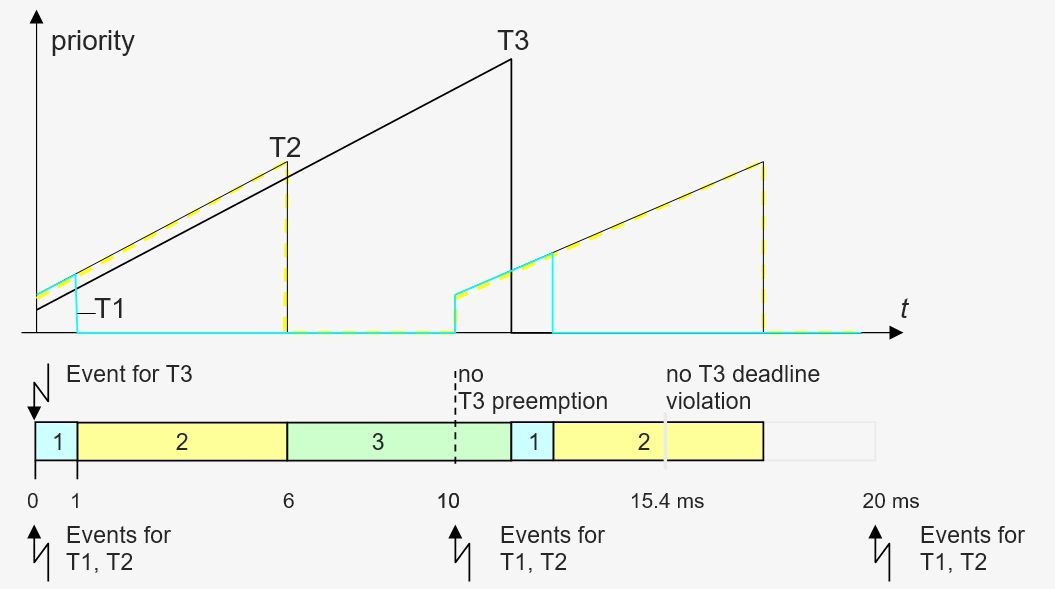
\includegraphics[width=13cm, height=6cm]{Images/image101.png}
    %\caption{}
    \label{fig:Fig 47}
    \end{figure}

(at \textit{t} = 0, T1 and T2 have equal priorities, due to equal deadlines, in such a case, the scheduler decides randomly, e.g. for the task with the lower id)\\

It can be seen, that with EDF scheduling an executable schedule is found. \\

Liu [W\"{o}rnB] shows, that EDF scheduling is an optimal scheduling with\\

\begin{equation}
	H \mathrm{<} 100 \% for\ preemptive\ EDF\ scheduling
\label{EQ }
\end{equation}

\textbf{Advantage}: 

\begin{enumerate}
\item  as long as the processor utilization is less than 100 \% with a uniprocessor system, EDF  scheduling delivers an executable schedule and compliance with all time conditions is guaranteed.
\end{enumerate}

\textbf{Disadvantages:}

\begin{enumerate}
\item \textbf{ }increased computational complexity for the dynamic priorities needed at run time.

\item  the sequence of task assignment is difficult to control.

\item  the time of execution is difficult to control with fixed time requirements.
\end{enumerate}
\newpage

\section{Task-Synchronization and Communication}

As most of the resources may only be used exclusively, tasks that request these resources must be synchronized for exclusive use, sometimes with regard to some sequence of access. \\

Thus, the OS provides \textbf{means for} \textbf{synchronization} either for 

\begin{enumerate}
\item  mutual exclusion, and 
\item  cooperation (sequence of access).
\end{enumerate}

{\rot\bf Synchronization }\\

The problem of synchronization of tasks arises when these tasks are not independent from each other. Dependencies arise, when common resources are be used, then the access needs to be coordinated. Common resources may be

\begin{enumerate}
	\item  \textbf{Data: }Multiple tasks read and write access to shared variable, like tables. (without synchronization, uncoordinated access could result in inconsistent data, e.g. when task 1 is reading values of a table, while another task 2 is updating that table partly.

	\item  \textbf{Devices: } Multiple tasks using common devices such as sensors or actuators. (again, coordination is necessary to not to send e.g. contradictional commands of two tasks to a stepper motor drive).

	\item  \textbf{Programs: } Several tasks share common programs, such as device drivers. Competing calls to a device driver must be assured to leave consistent application states.
\end{enumerate}

\textbf{ Example}: Two tasks compete for access to a data table:\\

task 1 is reading several temperature sensors, and stores these values in a table\\
task 2 is reading this table, and prints out the temperature distribution.\\

Without synchronization, this can lead to erroneous results if, for example task 1, the common table has not yet been fully updated, while task 2 accesses. Then, task 2 gets mixed new and old temperature values, which can lead to undefined states !

 	\begin{figure}[h]
    \centering
    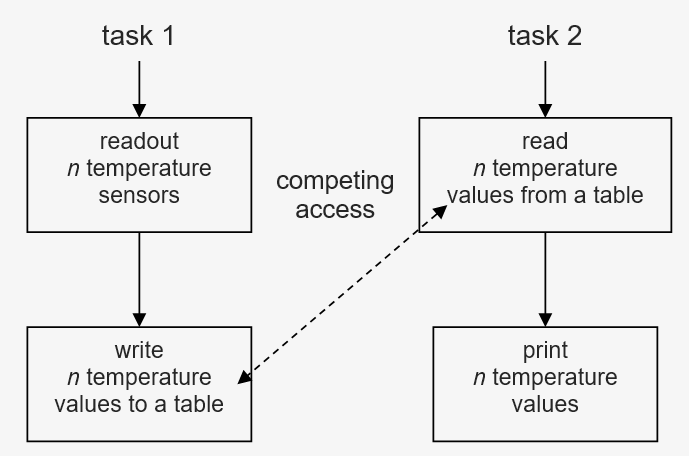
\includegraphics[width=9cm, height=6cm]{Images/image102.png}
    %\caption{}
    \label{fig:Fig 48}
    \end{figure}

\newpage  
There are two basic types of synchronization:

\begin{enumerate}
\item The \textbf{Mutual Exclusion }or shortly called \textbf{\textit{Mutex}}, ensures that access to a common resource is permitted only to one task at a time. 

 	\begin{figure}[h]
    \centering
    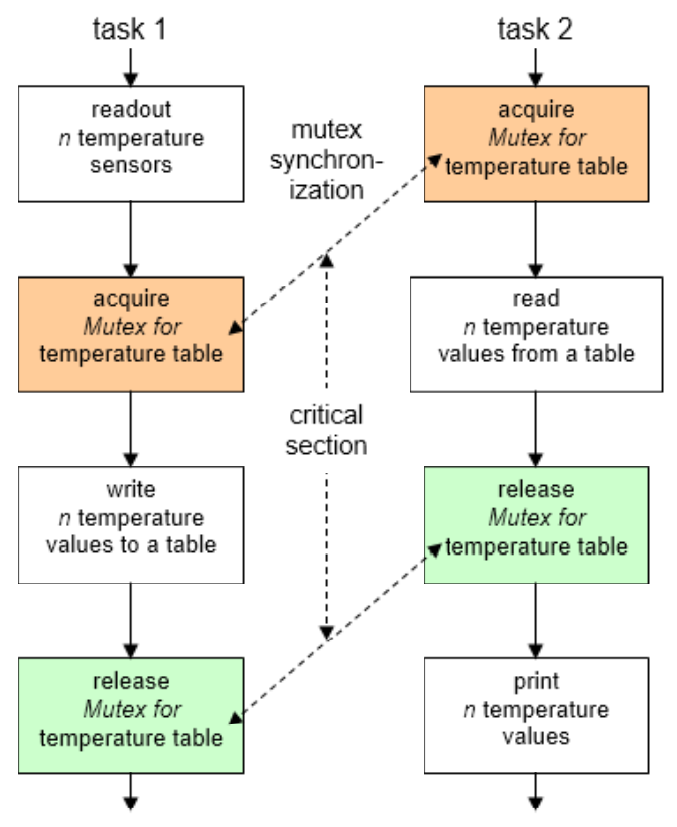
\includegraphics[width=9cm, height=9cm]{Images/image103.png}
    %\caption{}
    \label{fig:Fig 49}
    \end{figure}

\textbf{Example:} of temperature measurement using the \textbf{mutex} synchronization.\\

\textbf{ }For the protection of the common temperature table, a \textbf{mutex} is defined, toexclude the possibility that both tasks \textbf{access} this resource simultaneously.Before entering the critical section a task tries to acquire the mutex from the OS. If the mutex is already occupied by the other task, the newly accessing task is blocked\textbf{\textit{ }}until the other task \textbf{releases} the \textbf{mutex} again. The task will \textbf{un-block,} acquisition of the \textbf{mutex} succeeds, allowing the task to enter the critical section.\\

The sequence, which task 1 or 2 acquires the \textbf{mutex} does not matter.

\item Synchronization, where the order of access to common resources matters is called \textbf{cooperation} --unlike as with\textbf{ mutex synchronization}, which doesn't regard the order of task requests.

 	\begin{figure}[h]
    \centering
    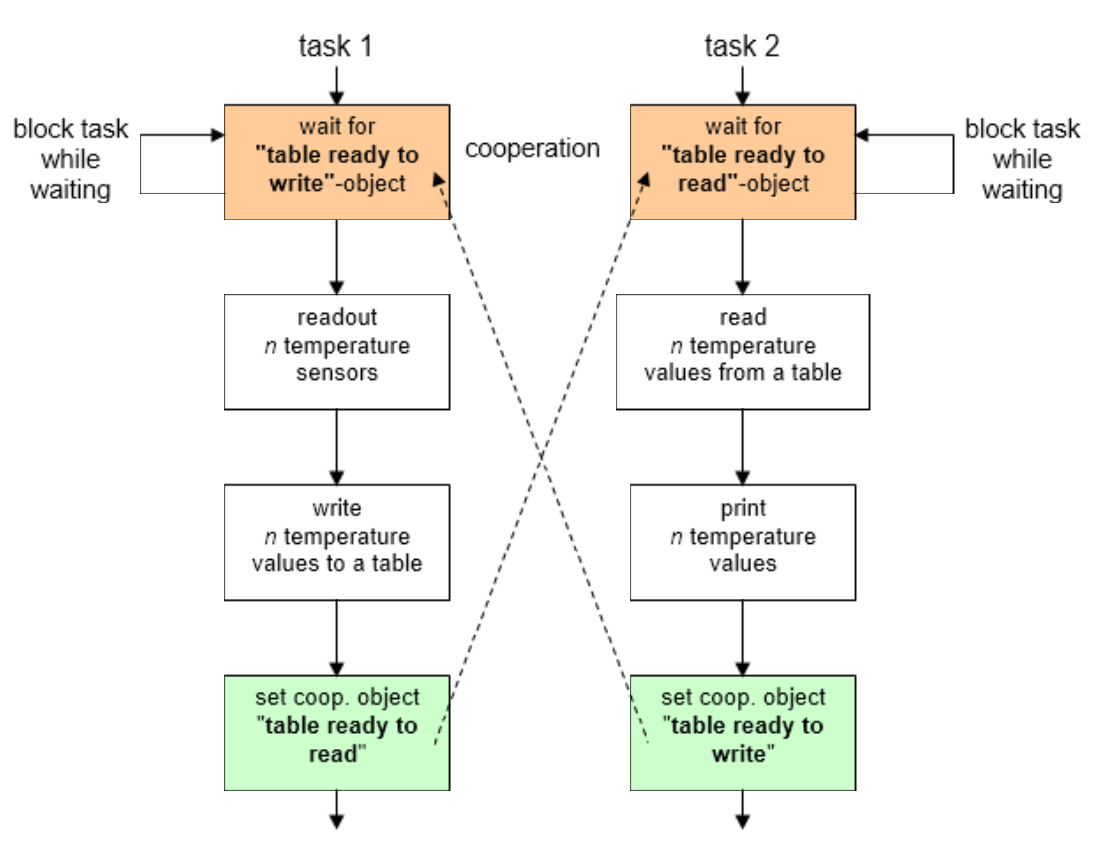
\includegraphics[width=14cm, height=10cm]{Images/image104.png}
    %\caption{}
    \label{fig:Fig 50}
    \end{figure}
    
Both, mutex synchronization and cooperation objects can be realized with semaphores.
\end{enumerate}
\newpage

\subsection{Semaphores}

A semaphore (from the Greek $\sigmaup$ $\muup$ $\alphaup$ = "sign" and $\varphiup$ $\varepsilonup$ $\rhoup$ $\varepsilonup$ $\iotaup$ $\nuup$ ="carry") is historically a signal mast or flag signal, in Information Technology it is an object for synchronization of processes.


A \textbf{semaphore} is basically a counter variable and two non-interruptible \textbf{operations}:  

\begin{enumerate}
\item  \textbf{Acquire}   (also called "\textbf{take}", "\textbf{signal}",  "\textbf{lock}",     or "\textbf{Passieren}", (\textbf{P}))
\item  \textbf{Release}  (also called "\textbf{give}", "\textbf{wait}",  "\textbf{unlock}"  or "\textbf{Verlassen}", (\textbf{V}))
\end{enumerate}

If a task tries to \textbf{\textit{acquire}} a semaphore, an associated counter variable is decreased. As long as the counter variable has a value less than 0, then the acquiring task is blocked.\\

Thus, during initialization the positive value of the semaphore states the number of tasks -waiting in a FIFO queue, or in a list using priorities- that may pass the semaphore, and thus enter the critical region protected by the semaphore.\\

If a task \textbf{\textit{releases}} a semaphore the associated counter variable is increased again. If the value of the counter variable is smaller than 1, tasks trying to acquire the semaphore are blocked, or, if the counter is greater or equal than 1, a waiting task is released from its blocking state  the task gets ready.Thus, a negative semaphore counter value indicates the number of tasks that have been prohibited to pass a semaphore. \textbf{Binary semaphore} only use \textbf{0} and \textbf{1} as counter values.

 	\begin{figure}[h]
    \centering
    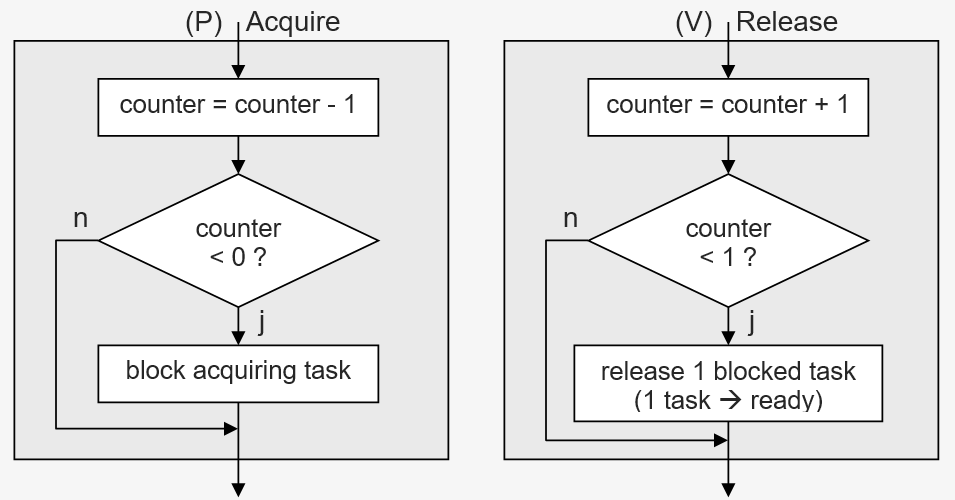
\includegraphics[width=12cm, height=5cm]{Images/image105.png}
    %\caption{}
    \label{fig:Fig 51}
    \end{figure}

It is of crucial importance that the operations "Passieren" and "Verlassen" (as originally introduced by Dijkstra) are realized atomically, i.e. they cannot be interrupted by any other operation. Only then, a consistent handling of the counter variable is ensured. Semaphore objects are managed by the RT-OS.\\

\textbf{Other names} for the \textbf{semaphore operations}:

P(sem) = Passieren(sem) = sem.P() = sem.decrement() = sem.wait() = take(sem)${}_{VXWorks}$

V(sem) = Verlassen(sem) = sem.V() = sem.increment()  = sem.signal() = give(sem)${}_{VXWorks}$\\


For \textbf{mutex-synchronization} a semaphore is used, with counter initialized with 1. Therefore, only one task can pass, gaining access to the protected resource: 

 	\begin{figure}[h]
    \centering
    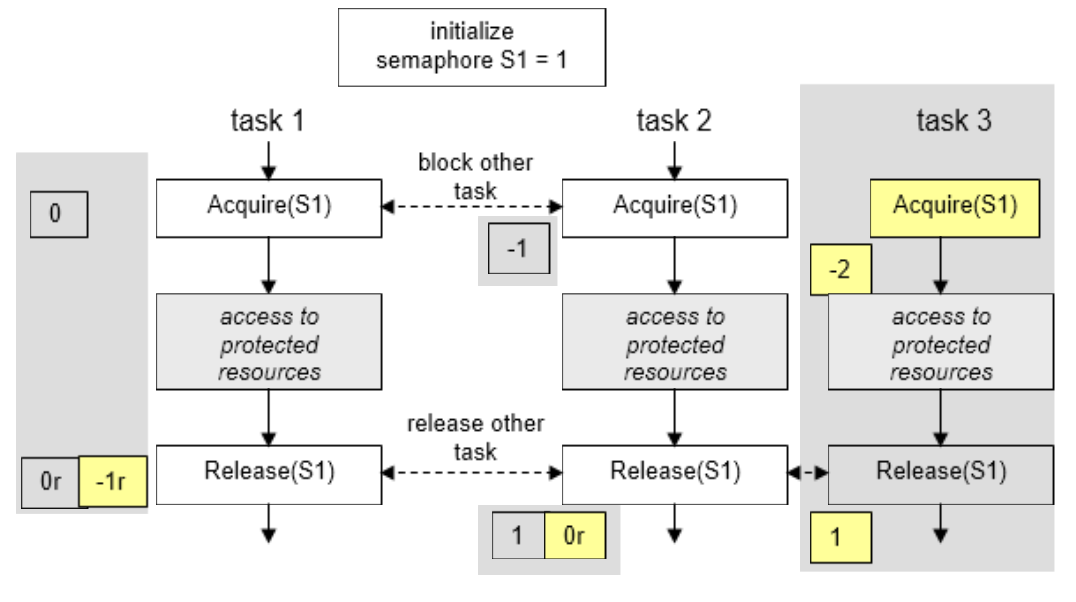
\includegraphics[width=14cm, height=7cm]{Images/image106.png}
    %\caption{}
    \label{fig:Fig 52}
    \end{figure}


\textbf{Example: Semaphore as Mutex in FreeRTOS}

\begin{lstlisting}[style=mystyle, language=c]
xSemaphore semAD;									// a global Semaphore
int table[16];										// a table of 16 temperatures

void vAppTask(void * pvParameters)
{
	semAD = vSemaphoreCreateBinary();		// Create a Semaphore, initially 1 

	while(1) {
		...
		xSemaphoreTake(semAD,portMAX_DELAY);		// <---- sync aquire mutex
		
		// read temperatures exclusicely ...
		Read_Temperatures(table);

		xSemaphoreGive(semAD,portMAX_DELAY);		// <---- sync release the mutex
 	}
}

void vPrintTask(void * pvParameters)
{
	while(1) {
		...
		xSemaphoreTake(semAD,portMAX_DELAY);	// <---- sync aquire mutex
		
		// print the table of temperatures exclusicely ...
		Print_Temperatures(table);

		xSemaphoreGive(semAD,portMAX_DELAY);	// <---- sync realease the mutex !
 	}
}
\end{lstlisting}

A \textbf{cooperation synchronization} can be realized by means of two semaphores. Example: sequential order of a task cooperation T2T1T2 with 2 semaphores:

 	\begin{figure}[h]
    \centering
    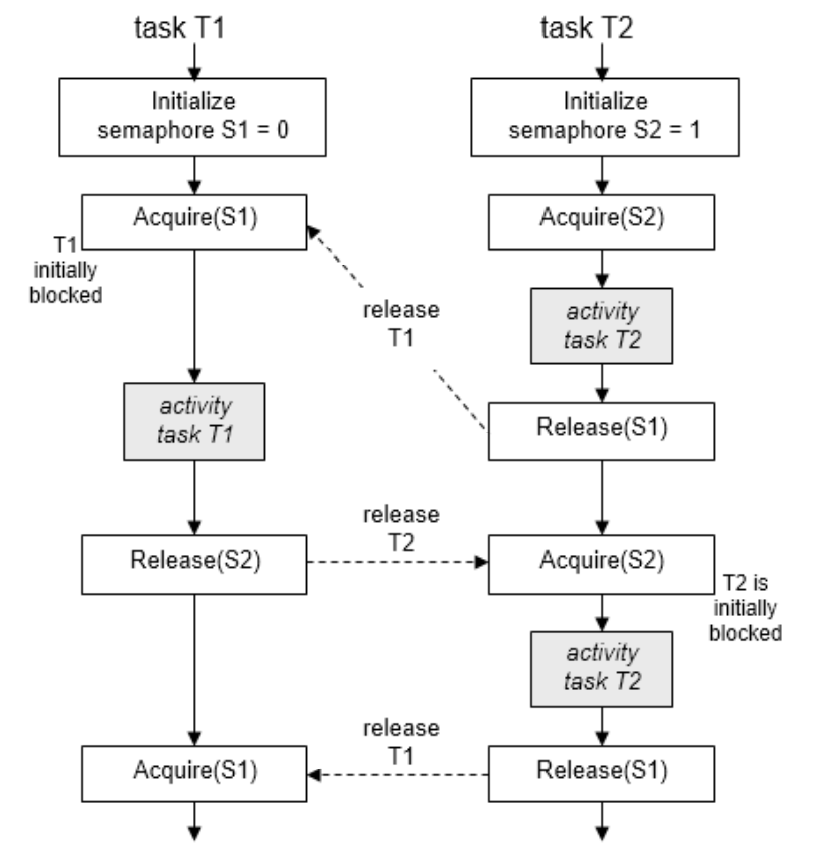
\includegraphics[width=11cm, height=12cm]{Images/image107.png}
    %\caption{}
    \label{fig:Fig 53}
    \end{figure}
\newpage
\textbf{Example: Cooperation in FreeRTOS  }

\begin{lstlisting}[style=mystyle, language=c]
void init()
{
	s1 =	vSemaphoreCreateBinary();			// Create a binary Semaphore 
	s2 =	vSemaphoreCreateBinary();			// Create a binary Semaphore 
	initSemaphore(s1,0);  	
	initSemaphore(s2,1);
}

void vTask1(void * pvParameters)
{
	while(1) {
		xSemaphoreTake(s1,portMAX_DELAY);	// <---- sync take blocks task !
		t1_activity();						// main T1 activity
		xSemaphoreGive(s2,portMAX_DELAY);	// <---- sync 
 	}
}

void vTask2(void * pvParameters)
{
	while(1) {
		xSemaphoreTake(s2,portMAX_DELAY);	// <---- sync take blocks task !
		t2_activity();						// main T1 activity
		xSemaphoreGive(s1,portMAX_DELAY);	// <---- sync 
 	}
}
\end{lstlisting}

\subsection{Deadlocks}

Synchronization of tasks can lead to a deadlock (\textbf{\textit{block}}, \textbf{\textit{deadly embrace}}), a situation, where the continuation of one or more tasks is blocked permanently. A simple example of a deadlock is an intersection with right-before-left right-of-way rule and four simultaneously arriving vehicles. After the priority rule any vehicle must wait for being right to another one, none of the Vehicles can drive. Only a break of the rule can release the deadlock.In task management, there are two types of deadlocks: deadlocks and livelocks.\\

In a deadlock tasks waiting on the release of resources for which they block each other. This leads to a standstill of the waiting tasks. The previous example with the traffic intersection describes such a deadlock.\\

Deadlocks typically occur when multiple resources are to be protected at the same time over cross:

 	\begin{figure}[h]
    \centering
    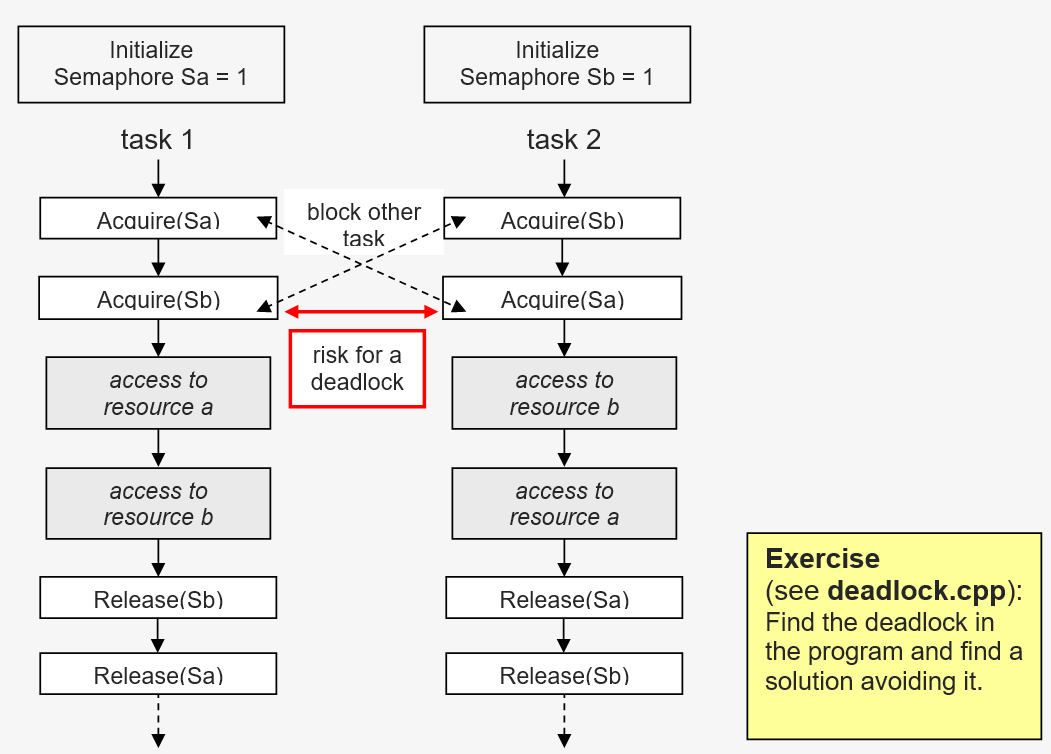
\includegraphics[width=12cm, height=11cm]{Images/image108.png}
    %\caption{}
    \label{fig:Fig 54}
    \end{figure}

In the above program there is a risk for a deadlock, since whenever both tasks are executed nearly parallel in time, both semaphores Sa and Sb are acquired, but never released. Deadlocks are usually realized unintended, i.e. as \textbf{\textit{software bugs}} !\\

A simple rule to avoid deadlocks:

\begin{tcolorbox}[colback=blue!5!white,colframe=blue!75!black]
	If several resources are to be protected at the same time, all accessing tasks must acquire / release semaphores in the same order to avoid deadlocks.
\end{tcolorbox}

Another, although less elegant, method is to remove deadlocks already occurred, by a defined waiting period for any task in blocked state, a so-called \textbf{\textit{timeout}}. If, after the time-out, a task is still in blocked state, that task is reset and all depending resources it occupied are released. This technique is implemented in some RTOSes, see also $\rightarrow$ Software Watchdog concept.

\subsection{Livelocks}

Livelocks (starvation) designate a condition in which a task is constantly inhibited from running by the conspiracy of other tasks. For example, when using a fixed lower-priority task never can get the processor due to the constant activity of higher-priority tasks.\\

\textbf{Example} FPP, task 1\textbf{: high priority}, task 2:\textbf{ low priority}, task 3:\textbf{ medium priority}

 	\begin{figure}[h]
    \centering
    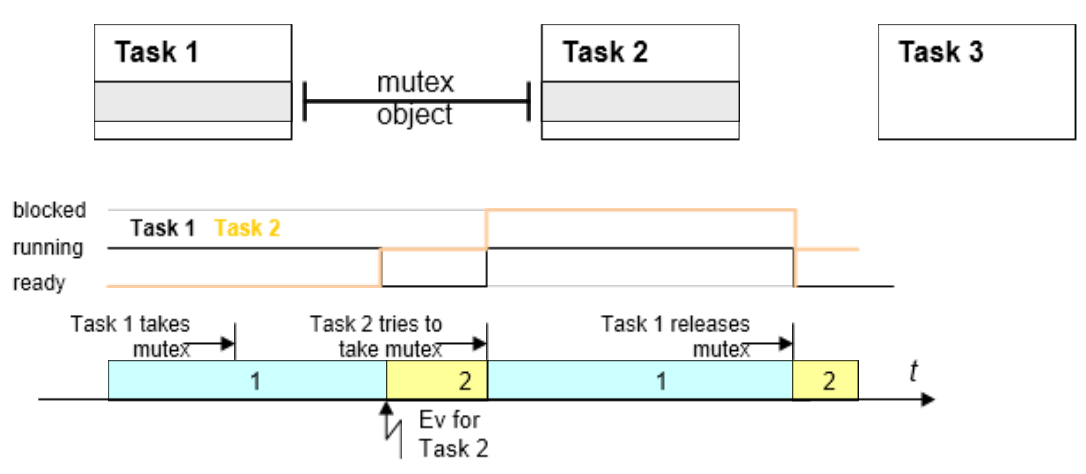
\includegraphics[width=12cm, height=6cm]{Images/image109.png}
    %\caption{}
    \label{fig:Fig 55}
    \end{figure}

However, this can also happen in high-priority tasks, provided that a \textbf{\textit{priority inversion}} occurs: the high-priority task 1 is livelocked by the lower priority tasks 2 and 3:

 	\begin{figure}[h]
    \centering
    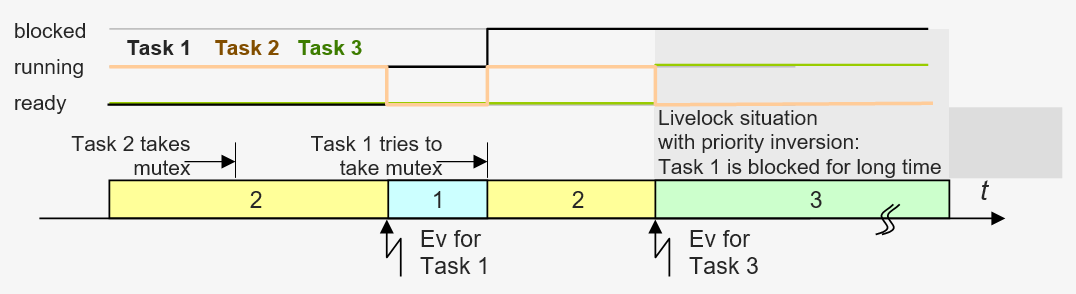
\includegraphics[width=12cm, height=4cm]{Images/image110.png}
    %\caption{}
    \label{fig:Fig 56}
    \end{figure}
\newpage
The problem of livelock by priority inversion can be solved by the technique of \textbf{priority} \textbf{inheritance} [W\"{o}rnB]   in the example above: task 2 inherits the high priority of task 1 (both wait for the same mutex), such that task 2 running in the critical section cannot be interrupted by a medium priority task 3. \\

A priority inversion condition occurs when a high-priority task must wait for synchronization objects of a lower-priority task (with \textbf{fixed priority scheduling}). This was the problem of the 1997 Mars mission "Sojourner" (running VxWorks), which was finally rescued by a watchdog [W\"{o}rnB] .


\subsection{Task Communication}

Synchronization and communication tasks are very closely related. \textbf{Synchronization} can be thought of as\textbf{ communication without information}. On the other hand, communication can be used for synchronization.\\

An example could be waiting for an order. With the order, information is transmitted, and by the time the order is sent, synchronization is possible (the job can start actually).\\

There are two basic variants of the task communication:

\begin{enumerate}
	\item  \textbf{Shared memory: } \\
	The data exchange is via a shared memory.\\
	The synchronization at what time read or write access occurred is done by a semaphore.
	\item  \textbf{Messages (Events): }The data exchange and synchronization is done via sending messages.
\end{enumerate}

In general, the communication via shared memory is faster than communication via messages. Therefore, this variant is preferred used in real-time operating systems. \\

In spatially \textbf{\textit{distributed systems}}, this is not possible because there is no physically shared memory. Here communication must take place via messages ($\rightarrow$ message queues).
\newpage
\subsection{Events}

With a mutex synchronization the access of competing tasks to a jointly used resource was enabled. \\

In contrast, for cooperating tasks time (and order) of execution has to be synchronized. This can be done by semaphores, but also with a simpler concept, an \textbf{\textit{event}}.\\

A task can wait on an \textbf{\textit{event}} (event wait), which is set by another task. Once set, the waiting tasks gets released from its blocking state.\\

\textbf{Example}: \\
Each of 3 tasks (task A, task B, task C) acquires a measurement value, which shall be processed by a 4${}^{th}$ task W. If A, B or C has acquired a measurement value, this is written to a data memory ("datenspeicher"), which can store exactly one value. Task W retrieves its input from that data memory.

 	\begin{figure}[h]
    \centering
    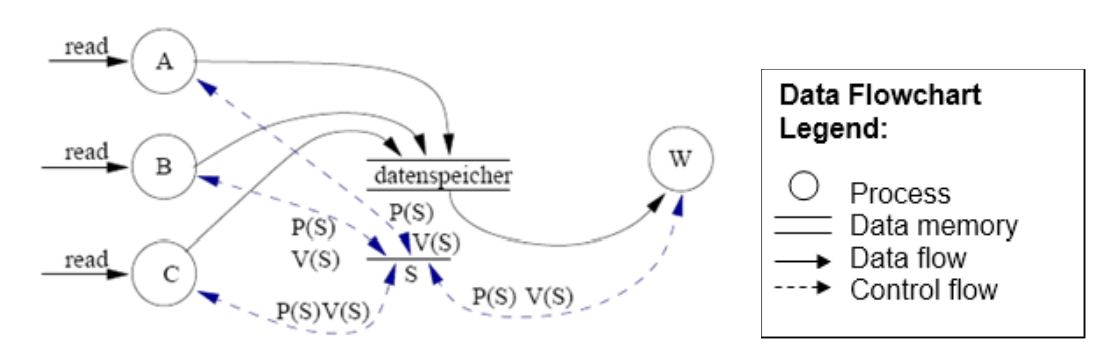
\includegraphics[width=13cm, height=4cm]{Images/image111.png}
    \caption{Data flow of an acquisition of measurement values: synchronization without events}
    \label{fig:Fig 57}
    \end{figure}

Since the data memory (datenspeicher) is existing only once, it is a shared resource, and access to it is a critical section, which can be protected by a semaphore S\\

\begin{lstlisting}[style=mystyle, language=c]
// Task A,B und C
	...
	while( TRUE ) {
  	read(kanal_A, buffer, sizeof(buffer));
  	P(S); // enter critical section
  	write( datenspeicher, buffer, sizeof(buffer));
 	 V(S); // leave critical section
}
...
}
\end{lstlisting}

\begin{lstlisting}[style=mystyle, language=c]
// Task W
...
while( TRUE ) {
  	P(S); // enter critical section
 	 read(datenspeicher, buffer, sizeof(buffer));
  	V(S); // leave critical section
 	 WorkOnData( buffer );
}
\end{lstlisting}

\textbf{Problems} with synchronization without events:

\hspace{1cm} \textbf{the data memory} can be overwritten, without being read before by W
 
\hspace{1cm} W can read the \textbf{data memory} repeatedly.\\

Therefore, it is not sufficient to protect the shared resources by using a semaphore, yet another synchronization means is necessary: an \textbf{\textit{event}}.

\begin{tcolorbox}[colback=blue!5!white,colframe=blue!75!black]
 \textbf{Definition: }\\ An \textbf{event} is a synchronization object, which allows computing processes to give free the processor (by going to the \textbf{block}-state), up to a certain condition is met.
\end{tcolorbox}

\textbf{Basic operations} of the \textbf{event} are:\\

\hspace{1cm}  Wait for an event, and

\hspace{1cm}  Send an event.\\

An \textbf{event} can\textbf{ get "lost"}, if an event is sent when no process waits on it  !\\
Since events are not stored -unlike semaphores-, events are used often in combination with a semaphore.

 	\begin{figure}[h]
    \centering
    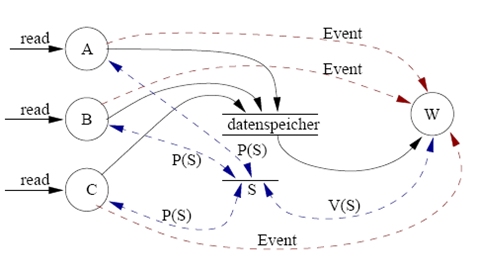
\includegraphics[width=10cm, height=4.5cm]{Images/image18.png}
    %\caption{}
    \label{fig:Fig 58}
    \end{figure}

Data flow of an acquisition of measurement values: synchronization with events

In order to grant access to the data for the tasks A, B or C only, after task W has emptied the data memory, the operation "enter critical section" and "leave critical section" is distributed to different tasks, similar to cooperation synchronization with semaphores.\\

Each of the tasks A, B and C enters the critical section (by calling the "P(S)"-operation), but never "leaves the critical section" by itself, this release is now done by task W (by calling the "V(S)"-operation). Task W must now be synchronized, so that it fetches the data from memory only, if these are available. Thus, Task A, B or C send an event on which task W is waiting:\\

\begin{lstlisting}[style=mystyle, language=c]
// Task A,B und C
...
read(kanal_A, buffer, sizeof(buffer) );
P(S); // enter critical section
write( datenspeicher, buffer, sizeof(buffer) );
SendEvent( Task_W );
...
\end{lstlisting}

\begin{lstlisting}[style=mystyle, language=c]
// Task W
while (1) {
  WaitForEvent( Task_W );
  read( datenspeicher, buffer, sizeof(buffer) );
  V(S); // leave critical section after read
  WorkOnData( buffer );
}
\end{lstlisting}

The critical section is thus defined from the time which an acquiring task A,B, or C writes a value into the data memory, until task W has read the value out of the memory.\\

\textbf{Problem}: Events can get lost, if sent when no task is waiting

 	\begin{figure}[h]
    \centering
    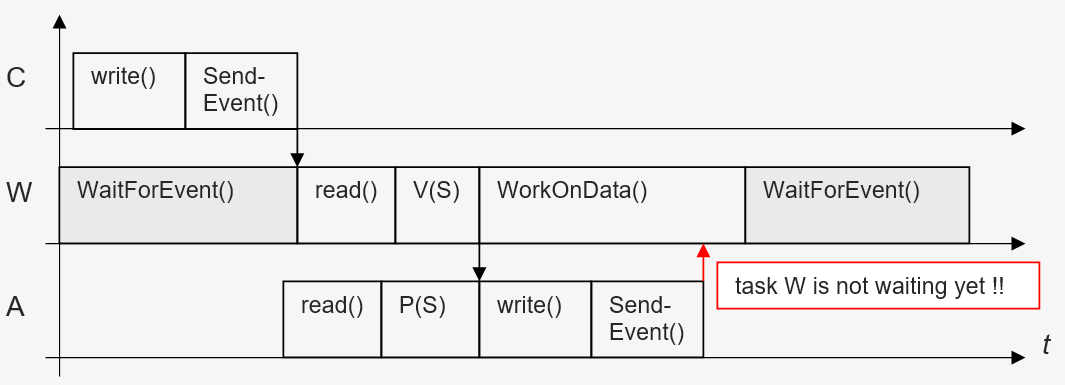
\includegraphics[width=14cm, height=4.5cm]{Images/image112.png}
    %\caption{}
    \label{fig:Fig 59}
    \end{figure}

\begin{itemize}
	\item task C causes task W to get running, starting with read()
	\item During read() in task W, task A has read new data
	\item task A is blocked by P(S), before W could release the semaphore
	\item task W releases V(S)
	\item task A continues with write() and SendEvent()
	\item the event gets lost, cause task W is busy WorkingOnData(), not waiting:  \textbf{\textit{critical race condition !!}}
	\item data loss A.
\end{itemize}
  
\textbf{Solution}: Move he WorkOnData() call into the critical section:

\begin{lstlisting}[style=mystyle, language=c]
// Task W
while (1) {
  WaitForEvent( Task_W );
  read( datenspeicher, buffer, sizeof(buffer) );
  WorkOnData( buffer );
  V(S); // leave critical section after work
}
\end{lstlisting}

Now, with this solution, the conflict is solved, since immediately after the critical section is left, task W can wait for events there is no more critical race condition:

 	\begin{figure}[h]
    \centering
    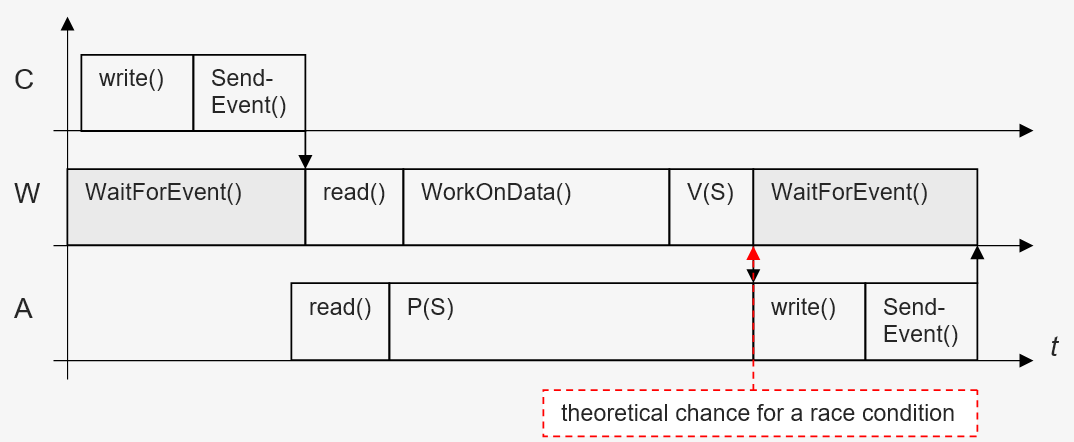
\includegraphics[width=14cm, height=4.5cm]{Images/image113.png}
    %\caption{}
    \label{fig:Fig 60}
    \end{figure}

Since there is a theoretical (although very small) chance, \textbf{Posix} defines an atomar, non-interruptable operation combining the semaphore release and waiting on an event:

 	\begin{figure}[h]
    \centering
    \includegraphics[width=10cm, height=1cm]{Images/image114.png}
    %\caption{}
    \label{fig:Fig 61}
    \end{figure}
    
\begin{lstlisting}[style=mystyle, language=c]
// Task W
P(S); // since WaitForEventAndV releases a semaphore
      // this most be locked (acquired) first
while(1) {
  read( datenspeicher, buffer, sizeof(buffer) );
  WorkOnData( buffer );
  // V(S); leave critical section after work, done above
  WaitForEventAndV(S); // Release semaphore and wait
}
\end{lstlisting}

\begin{lstlisting}[style=mystyle, language=c]
// Task A,B und C
...
read(kanal_A, buffer, sizeof(buffer) );
P(S); // enter critical section
write( datenspeicher, buffer, sizeof(buffer) );
SendEvent( Task_W );
...
\end{lstlisting}

\textbf{Posix Functions:}\\

By these functions a critical section is entered, and left\\

P(S):  int \textbf{pthread\_mutex\_lock }( pthread\_mutex\_t * \textit{mutex });

V(S):  int \textbf{pthread\_mutex\_unlock}( pthread\_mutex\_t * \textit{mutex });\\


WaitForEventAndV(S):

int \textbf{pthread\_cond\_wait}( pthread\_cond\_t * \textit{cond }, pthread\_mutex\_t * \textit{mutex });

\textbf{Alternative Solution: increase Memory, use }Message Queues \textbf{as a standard solution !}

\subsection{Signals}

Signal are very similar to events. Signals can be processed asynchronously to the program (call of a signal-handler routine), with events the processing is synchronous (\textbf{wait\_for\_event}() - functions as part of the program).

\begin{itemize}
\item Signals are often used in UNIX programs. 
\item Signals they can be seen as software interrupts at the application level.
\end{itemize}

\subsection{Messages Queues, Mailboxes}

\textbf{Message queues} provide an asynchronous communication protocol, which means that the sender and receiver of the message must not interact simultaneously. Messages will be placed on a queue, where they are stored until the recipient retrieves one or more by a FIFO mechanism. The maximum amount of data a single message is usually limited.\\

A message queue without a restriction for the number of messages is called \textbf{mailbox}.

 	\begin{figure}[h]
    \centering
    \includegraphics[width=14cm, height=3cm]{Images/image115.png}
    %\caption{}
    \label{fig:Fig 62}
    \end{figure}
\newpage    
\textbf{Example}: FreeRTOS - Queue (www.freertos.org)

\begin{lstlisting}[style=mystyle, language=c]
#include <FreeRTOS/queue.h>
...
struct AMessage
{
	portCHAR ucMessageID;
	portCHAR ucData[ 20 ];
}

xQueueHandle xQueue1;

void vATask(void *pvParameters)
{
	// Create a queue capable of containing 10 pointers to AMessage structures.
	// These should be passed by pointer as they contain a lot of data.

	xQueue1 = xQueueCreate( 10, sizeof( struct AMessage * ) );
}

...

// -------------------------  send from any task ----------------------------}
{
 	// Send a pointer to a struct AMessage object.  Don't block if the
  	// queue is already full.
 	struct AMessage *pxMessage;

 	pxMessage = \& xMessage;
	xQueueSend( xQueue1, (void *) \&pxMessage, (portTickType) 0 );
}
...

// ------------------------- receive with any task --------------------------}

{  
	// Receive a message on the created queue.  Block for 10 ticks if a
	// message is not immediately available.
	struct AMessage *pxMessage;
	if( xQueueReceive(xQueue1, \&(pxRxedMessage), (portTickType ) 10 ))
	// pcRxedMessage now points to the struct AMessage variable posted

}
\end{lstlisting}

The \textbf{QueueReceive()} command places the calling task into the \textbf{\textit{blocked (waiting)}} state if the message queue is empty. If not, it returns the object to which the read (out-) pointer points to, and the read (out-) pointer set to the next message object.\\

The \textbf{QueueSend()} command places the calling task into the blocked (waiting) state only, if the message queue is full. If not, the object is being stored at the position the write (in-) pointer references, and the pointer is set to the next free space in which the next transmitted (posted) message object is stored.\\

In many RTOS, a maximum blocking time can be specified (as with FreeRTOS).\\

Lab-experiment "Message Queue with ARM LPC4357 µC (FreeRTOS)"

\subsection{Socket Interface}

The most important interface for inter-process communication on different computers connected via Ethernet, is the \textbf{socket interface}.\\

By using sockets, data can be exchanged between processes, which are located on different hosts (distributed system). \\

The socket interface provides access to TCP/IP (connection-oriented) and UDP/IP (connectionless) protocols for communications. \\

Once a socket connection between two processes has been established, the data can be exchanged with some basic system functions (open, read, write, close ...), the so-called \\

\textbf{Sockets Service Primitives}

 	\begin{figure}[h]
    \centering
    \includegraphics[width=12cm, height=5.5cm]{Images/image19.png}
    %\caption{}
    \label{fig:Fig 63}
    \end{figure}
    
$\rightarrow$ \textbf{ RTP ProgC Repetition Workspace}: ``\textbf{socket\_client, socket\_server}''\\

{\rot\bf Python Sockets Programming:}\\

The server connects to a client and echoes its message:

 	\begin{figure}[h]
    \centering
    \includegraphics[width=14cm, height=2cm]{Images/image188.png}
    %\caption{}
    \label{fig:Fig 64}
    \end{figure}
\newpage  
\textbf{(A) Server script }

 	\begin{figure}[h]
    \centering
    \includegraphics[width=16cm, height=9cm]{Images/image20.png}
    %\caption{}
    \label{fig:Fig 65}
    \end{figure}
   
First, the server executes LISTEN (line 12), and it remains blocked until a client connects. Then a client task executes CONNECT to establish a connection with the server (line 9). It must specify an IP address (the server's) and port number (must me common to both).\\

\textbf{(B) Client script }

 	\begin{figure}[h]
    \centering
    \includegraphics[width=16cm, height=5cm]{Images/image118.png}
    %\caption{}
    \label{fig:Fig 66}
    \end{figure}

The OS then sends an IP packet to the opposite computer (peer). The client process is blocked until the server responds.\\

If a confirmation is received, the client and server have established a connection and the connect() - or listen() function are released from blocking, and data can be exchanged until the end of the connection (close()).
\newpage

\section{Memory Management}

The main task of memory management is essentially providing access to the memory resource consisting of a hierarchy of cache, main memory (RAM), peripheral memory or NVRAM (non-volatile RAM, such as EEPROM) by

\begin{itemize}
	\item  the allocation of memory to the tasks,
	\item  the coordination of accesses to shared memory areas,
	\item  the protection of the storage areas of individual tasks
	\item  the displacement of memory areas
\end{itemize}

One can distinguish between different forms of memory allocation:

\begin{enumerate}
\item  \textbf{Static memory allocation: \\}The allocation of memory is made to a task before it is put into the \textbf{\textit{ready}} state. The memory allocation does not change at runtime.

\item  \textbf{Dynamic memory allocation: }\\The allocation of memory to a task is done at runtime and may change at any time.

\item  \textbf{Non-displacing memory allocation: }\\Allocated memory must not be withdrawn from a task at runtime.

\item  \textbf{Displacing memory allocation: }\\Allocated memory may be removed from a task at runtime, the memory is paged to peripheral memory (e.g. a swap-file).
\end{enumerate}

\textbf{Embedded systems} mainly use \textbf{static memory allocation}, since the dynamic allocation of memory is hardly predictable (and thus real-time compliant).Execution times of \textbf{malloc(), free(), new(), delete()}, .. can't be guaranteed to be smaller than a certain limit  availability.\\

The usage of an \textbf{MMU} (\textbf{M}emory \textbf{M}anagement \textbf{U}nit), which is quite common with many CPUs (x86, ARM Cortex A Series, ..), allows processors to deal with a virtual address space. Thus, memory access from the process is strictly separated from the OS and from other processes (= safety). However, with translation of the virtual addresses into physikalical addresses long delays can occur, which cannot be determined in advance! This is a contradiction to the required determinism with hard real-time requirements ! Thus, microcontrollers for applications having hard real-time requirements often do \textbf{\underbar{NOT}}\underbar{ have an MMU} and use \underbar{direct physical addressing} instead (AVR, ARM Cortex M Series, ..) 

 	\begin{figure}[h]
    \centering
    \includegraphics[width=12cm, height=2.5cm]{Images/image119.png}
    %\caption{}
    \label{fig:Fig 67}
    \end{figure}
    
\section{Input/Output Management (I/O)}

Along with task- and memory-management the\textbf{ }I/O-management is the 3${}^{rd}$  important component of a real-time operating system, especially with embedded systems, where I/O tasks for sensors and actors have hard real-time requirements.\\

In addition to that, synchronous an asynchronous serial interfaces, and networking subsystems require high performance I/O-management.\\

{\rot\bf I/O Basics}\\

The tasks of the I/O-management can be divided into two groups:

\begin{itemize}
\item  assigning and sharing of devices for the tasks
\item  use of assigned and shared devices by the tasks
\end{itemize}

The connected devices differ greatly in speed and data format. The OS has therefore the task, to abstract from implementation details and provide a \textbf{simple, uniform and transparent interface}. \\

This can be achieved by a multi-layer architecture of the I/O management:

 	\begin{figure}[h]
    \centering
    \includegraphics[width=6cm, height=4cm]{Images/image189.png}
    %\caption{}
    \label{fig:Fig 68}
    \end{figure}
    
The main 2 layers of I/O-management:

\begin{enumerate}
\item  \textbf{I/O-Control: }\\This layer is above the layer of the device driver and interfaces with the tasks.It is hardware independent, i.e. implementation and operation is no longer depending on the type of connected devices. It takes care for data transport, data format, data buffering, and messaging. If a certain device needs to be exchanged, its device driver needs to be exchanged too, but not the I/O control.The I/O control abstracts from the specific devices and provides a \textbf{simple, uniform and transparent interface} to the \textbf{tasks}.

\item   \textbf{Device Driver:}\\The device driver is a layer next to the hardware, i.e. its realization depends on the connected devices. It takes into account all device-specific properties, including direct communication with the devices. It produces all necessary control signals, evaluates the status signals andhandles the device's interrupts. The device driver monitors all transfers, and possibly do some error handling, e.g. evaluate parity bits and initiate the repetition of a failed transmission.
\end{enumerate}

\textbf{Example}: I/O-management of a hard disk drive:\\

Each drive has a unique device driver, that takes into account their specific characteristics such as speed, number of heads, cylinders and sectors. At the level of I/O-control, each disk is treated equally, for the task addressing of data is done by a block number, abstracted from the device-specific parameters: \\

\textbf{FILE *fp =  fopen("c:{\textbackslash}test.bin"); fseek(fp, {\dots}), fwrite(fp, {\dots}), fclose(fp);}\\

Typical interface functions provided by the\textbf{ }I/O control layer

\begin{table}[h!]
\setlength{\tabcolsep}{10pt} % Default value: 6pt
\renewcommand{\arraystretch}{1.5} % Default value: 1
\centering
 \begin{tabular}{|c|c|c|c|} \hline
 \textbf{Function} & \textbf{Description} \\ [0.1ex] 
Create & Creates a virtual instance of an I/O device \\ \hline 
Destroy & Deletes a virtual instance of an I/O device \\ \hline 
Open & Prepares an I/O device for use \\ \hline 
Close & Communicates to the device that its services are no longer required, which \\ & typically initiates  device-specific cleanup operations \\ \hline 
Read & Reads data from an I/O device \\ \hline 
Write & Writes data into an I/O device \\ \hline 
Ioctl & Issues control commands to the I/O device (I/O control) \\ \hline 
 \end{tabular}
 %\caption{\textbf{}}
 %\label{Intrinsic}
\end{table}

The main functions of the I/O control layer are:

\begin{enumerate}
	\item  \textbf{Symbolic Names: }devices addressing by symbolic addresses, or names.
	\item  \textbf{Handling of I/O-Requests: }queuing, buffering I/O-requests  queues.
	\item  \textbf{Assignment of Devices: }assignment of the device (shared resource) to tasks dynamically or 	statically,using priorities for competing requests. 

	\item  \textbf{Synchronization: }I/O-requests affect a tasks state, (e.g. waiting  \textbf{\textit{blocked}} state), interface between I/O-control to task-management.

	\item  \textbf{Device Protection: } prevent unauthorized access by unauthorized tasks - protection against deadlocks and livelocks due to competing access- resets after programmable timeouts (protect against software failure).

	\item  \textbf{Communication with the device drivers: }forwarded executable device requests to the device driver, handle feedback, e.g., status or error codes 

	\item  \textbf{Buffering: }synchronization of different speeds of task-management and I/O-devices by temporary storage in buffer memory, handle buffter state events to the task/device

	\item  \textbf{Unique Data Format: }abstract from the device's physical data format, e.g. \textbf{endianness}.
\end{enumerate}

The boundary between I/O control and device drivers is floating and system dependent. For efficiency reasons with some RTOSes, functionality is moved into the device driver, which increases the effort for adapting new devices.\\

{\rot\bf Endianness}\\

The storage of the hexadecimal number 0x0A0B0C0D = 168496141 results in a different byte order in memory, dependent of the microcontroller or peripheral hardware:

 	\begin{figure}[h]
    \centering
    \includegraphics[width=13cm, height=2.5cm]{Images/image120.png}
    %\caption{}
    \label{fig:Fig 69}
    \end{figure}

\begin{enumerate}
\item  With \textbf{little-endian} hardware the least significant byte (\textbf{LSB}) is stored with the \textbf{lowest} \textbf{memory} (byte) \textbf{address}, 

\item  With \textbf{big-endian} hardware the most significant byte (\textbf{MSB}) is stored with the \textbf{lowest} \textbf{memory} (byte) \textbf{address}
\end{enumerate}

Most RTOS's provide functionality to abstract from \textbf{endianness} in the device driver. Example:

 	\begin{figure}[h]
    \centering
    \includegraphics[width=14cm, height=6cm]{Images/image121.png}
    %\caption{}
    \label{fig:Fig 70}
    \end{figure}

\subsection{I/O Synchronization}

The communication between peripheral devices and the processor is performed by interface devices\textbf{ }(\textbf{interface units}). These \textbf{interface devices} also define the base for synchronization between the processor (tasks), and devices operating at different speeds using certain registers:

 	\begin{figure}[h]
    \centering
    \includegraphics[width=12cm, height=4.5cm]{Images/image122.png}
    %\caption{}
    \label{fig:Fig 71}
    \end{figure}

The typical components of an interface device are:

\begin{enumerate}
	\item  \textbf{Data register(s)} to read/write the data to be received/transmitted.
	\item  \textbf{Control register(s)} for configuring the device (e.g. operating mode, speed of serial ports, e.g. UART).
	\item  \textbf{Status register(s)} reflecting the devices current state (e.g. sent data, received data bits, e.g. ADC).
\end{enumerate}

A running task can synchronize  (for changing data) with the interface device either by

\begin{enumerate}
	\item  Polling
	\item  Interrupts
\end{enumerate}

{\rot\bf Polling}\\

With the simplest synchronization method --polling- a task reads the status register continuously in a loop:

 	\begin{figure}[h]
    \centering
    \includegraphics[width=14cm, height=10cm]{Images/image123.png}
    %\caption{}
    \label{fig:Fig 72}
    \end{figure}

After initialization (by setting the control register) the task is waiting in an active loop on a status flag --which is a particular bit within the status register of the device- indicating that  data is available in the data register  

$\rightarrow$ the task reads the data from the data register.\\

\textbf{Advantages of polling:}\\

\hspace{1cm} Simple synchronization type\\

\textbf{Disadvantages of polling:}\\

\hspace{1cm} Consumption of processor time for the active loop

\hspace{1cm} Slow response times when multiple devices within a task are polled simultaneously.\\

\textbf{Conclusion}: Overall, polling is usually not favorable, due to inefficient CPU usage.\\
\newpage
{\rot\bf Busy Polling}\\

With busy polling, the properties of simple polling are improved with performing some activity (typically short) within the waiting loop:

 	\begin{figure}[h]
    \centering
    \includegraphics[width=14cm, height=9cm]{Images/image124.png}
    %\caption{}
    \label{fig:Fig 73}
    \end{figure}

A disadvantage is, however, the response time slows down. Longer activities must be split into smaller steps.\\

\textbf{Example (sampling system }(PWM-Control Experiment in Real-Time-Lab): 

\begin{itemize}
	\item  Start an AD converter process with known duration, 
	\item  Offset / Gain correction of previously read values,
	\item  Wait for the ADC to get ready,
	\item  Readout of the ADC data register.
\end{itemize}

 	\begin{figure}[h]
    \centering
    \includegraphics[width=6cm, height=4.5cm]{Images/image125.png}
    %\caption{}
    \label{fig:Fig 74}
    \end{figure}
\newpage
{\rot\bf Interrupts}\\

With synchronization by interrupts the interface executes an interrupt request with the processing CPU, which forces a currently running task to be interrupted in favor of a defined interrupt service routine \textbf{ISR}:

 	\begin{figure}[h]
    \centering
    \includegraphics[width=14cm, height=9cm]{Images/image126.png}
    %\caption{}
    \label{fig:Fig 75}
    \end{figure}

In the interrupt service routine (ISR), the data can be read from or written to the device.\\

\textbf{Advantage: }\\Processing time is consumed only, when data needs to be transferred\\

\textbf{Disadvantage: }\\Activating the ISR causes an overhead as the current processor state must be    saved for the old task to resume after return of the ISR    (equivalent to preemption with task-scheduling).\\

To reduce the effect of overhead, larger amounts of data are transmitted in blocks, usually in conjunction with direct memory access (DMA).\\

The technique of synchronization with interrupts is very well suited for real-time applications and thus interrupts are widely used with microcontrollers with both synchronous and asynchronous real-time programming.

\subsection{Interrupts and Task-Scheduling}

Interrupt handling in real-time operating systems raises the question, how these interruptions integrate with the task scheduling. On current processor CPUs a hardware interrupt causes the automatic invocation of an interrupt service routine (ISR). \\

The real-time operating system then has two options:

\begin{enumerate}
\item {\rot\bf Interruption of the Task-Oriented Processing: }

\begin{itemize}
	\item With an interrupt the currently running task is interrupted. The interrupt service routine (ISR) is executed immediately, after return the interrupted task continues.
\end{itemize}

\textbf{Advantage: } 

\begin{itemize}
	\item Very fast response to external events, because the interrupts are handled directly   by the CPU hardware.
\end{itemize} 

\textbf{Disadvantages: }

\begin{itemize}

\item The regular task-scheduling (eg EDF, FPP, TSS ...) is bypassed by direct handling   of the processor hardware.

\item The prozessor uses its own priority based preemption (FPP), might conflicting with real-time scheduling

 	\begin{figure}[h]
    \centering
    \includegraphics[width=14cm, height=5cm]{Images/image22.png}
    %\caption{}
    \label{fig:Fig 76}
    \end{figure}

\item Regardless of the scheduling strategy used by real-time scheduling events are treated with FPP scheduling, which can not guarantee 100\% processor utilization   (see section 2.2.7).

\item This kind of direct processing of interrupts with interruption of the task-oriented   processing is used for RTOS's with less performant microcontrollers,   better solution: integration of interrupts with task-scheduling.- The total available processor utilization for task-scheduled processing is reduced from originally 100 \% !
\end{itemize}

\item {\rot\bf Integration of Interrupts with the Task-Oriented Processing: }\\

There is a separate task, integrated with task-scheduling, which is responsible for interrupt processing. Thus, whenever the processor gets a hardware interrupt, the ISR starts that separate task, responsible for interrupts.\\

\textbf{Advantage: }

\begin{itemize}
	\item Interrupt handling is fully integrated with task-scheduling,   there are no more two schedulers simultaneously, which might conflicting.
	\item An interrupt has the same scheduling policy as all other tasks.   (e.g. an interrupt can have lower priority than the actually running task, such that it   is not interrupted, with solution 1, this is not possible).
\end{itemize}  

\textbf{Disadvantage: } 

\begin{itemize}
	\item The reaction to events is slowed, because the interrupt handling is not activated   directly by hardware any more, but by the task-scheduler.
\end{itemize} 

 	\begin{figure}[h]
    \centering
    \includegraphics[width=14cm, height=5cm]{Images/image23.png}
    %\caption{}
    \label{fig:Fig 77}
    \end{figure}

The integration of interrupts into the task-oriented processing is suitable for real-time operating systems using more powerful micro-controllers.
\end{enumerate}
\newpage

\section{Specialized RTOS}

\subsection{ Overview of some RTOS}

 	\begin{figure}[h]
    \centering
    \includegraphics[width=15cm, height=9cm]{Images/image127.png}
    %\caption{}
    \label{fig:Fig 78}
    \end{figure}

\subsection{ Classification of Real-Time Operating Systems}

For classifying RTOSes there can be made a separation into five basic types [1]:

\begin{enumerate}
\item  \textbf{Minimal Real-Time Operating System (MinOS)} 

\begin{itemize}
	\item Simple RTOS for microcontroller with limited memory resources.
	\item RTOS is a library, to be linked with the application.
	\item Simple I/O-functions No memory management, physical addressing only (no protected mode).
	\item threads only (lightweight processes)
\end{itemize}

\item  \textbf{Controller System (CS)} 

\begin{itemize}
	\item Minimal real-time operating system      \\ + a file system      \\ + better error handling.
\end{itemize}

\item  \textbf{Dedicated System (DS)}   
\begin{itemize}
	\item  Controller System      \\ + memory management.    \\ + protected mode.
\end{itemize}

\item  \textbf{Standard OS Extension (ExtOS)}
\begin{itemize}
	\item  Standard OS (Windows, Linux, ..)  \\ + some RTOS features
\end{itemize} 

\item  \textbf{Universal Real-Time OS (RTOS)} 
\begin{itemize}
	\item  Fully featured RTOS.  \\ + features of standard OS.
\end{itemize} 
\end{enumerate}

\subsection{Selection Criteria}

A first selection criterion is the classification described in 2.6, which is set by the scope and functionality of a real-time operating system (RTOS).\\

Other criteria selecting an RTOS are:

\begin{enumerate}
\item  \textbf{Development and Target Environment}

\begin{itemize}
	\item  Are there well-proven tools and libraries for both development and target ?
	\item Is the desired programming language supported (C, C++, ..) ?
	\item Smooth, reliable and fast communication process between the  target system and development system (re-flash cycle) ?
	\item What are the debug options and debugging tools on the target system  (E.g., source-level debugging)?
\end{itemize}

\item  \textbf{Modularity and Core Size}

\begin{itemize}
	\item  This criterion refers to the configuration and the memory requirements.
	\item Can the system be configured flexibly to the application ?
	\item Can it be restricted to the necessary components ? 
	\item What is the achievable size, application + libraries ?
\end{itemize}

\item  \textbf{Adaptability}

\begin{itemize}
	\item Is the RTOS adaptable for a particular microcontroller/peripherals ?
	\item How much effort is that adaption ?
	\item What field-bus systems or networks are supported ?
\end{itemize}

\item  \textbf{General Features}

\begin{itemize}
	\item What is the user interface of the operating system (GUI, cmd, None) ?
	\item Which libraries are part of the operating system ? (e.g. math, graphical, ...)
	\item What other tools are offered, (e.g. for version management, data management, ..)
\end{itemize}

\item  \textbf{Performance}\\ (usually a major criterion for selection). 
\begin{itemize}
	\item How large is the maximum number of tasks ?   (small automation app: 10 tasks, complex app: $\mathrm{>}$ 100 tasks)
	\item What task-scheduling methods are available ?
	\item What is the number of different priority levels ?
	\item What is the time for a context-switch ?
	\item What is the latency time with responding to interrupts ?
	\item For which class of real-time application the OS is designed ?  (e.g. can hard or firm real-time requirements be met ?)
\end{itemize}
\end{enumerate}

\subsection{ VxWorks}

VxWorks, by Wind River Company [2004], is a general purpose real-time operating system. In in its basic form, it supports no virtual memory ( $\rightarrow$ advanced product VxVMI).\\

VxWorks uses heavyweight processes as tasks. However, task-switch was optimized to enable fast task switching. \\

The context VxWorks stores in a task-control block (TCB) includes:

\begin{enumerate}
\item  the program counter of the task,

\item  the contents of processor registers and floating-point,

\item  the stack of the dynamic variables,

\item  the associated I / O devices,

\item  the signal handler and

\item  various debugging information
\end{enumerate}

The VxWorks state model for the tasks differs not much from the general model from section 2.1.3:

 	\begin{figure}[h]
    \centering
    \includegraphics[width=6cm, height=6cm]{Images/image128.png}
    %\caption{}
    \label{fig:Fig 79}
    \end{figure}

\begin{enumerate}
\item  \textbf{running} the task is executed (run).

\item  \textbf{ready} (ready) the task is ready to execute.

\item  \textbf{blocked} (pending) the task is waiting for the release of a resource and is blocked.

\item  \textbf{delay} (delayed) the task is stopped for a certain period of time.

\item  \textbf{suspended} (suspend) the task was suspended. This is intended for debugging purposes only.
\end{enumerate}

By default, VxWorks uses FPP scheduling. Each task is assigned an initial priority. This priority can be adjusted during runtime ( function \textbf{taskPrioritySet}() ).\\

VxWorks defines 256 priority levels, with 

\begin{enumerate}
\item  level \textbf{0} corresponding to the \textbf{highest}, and 

\item  level \textbf{255} to the \textbf{lowest priority}.
\end{enumerate}

The VxWorks task scheduler can be turned on and off explicitly by two functions (\textbf{taskLock() and taskUnlock()} ). The switch will prevent, that the current task is preempted by a higher priority task  realization of non-preemptive scheduling (FPN).\\

However, a task can still be interrupted by hardware interrupts. Deactivation of the task-scheduler is called \textbf{preemption locking}. It can be used for the protection of (short) critical sections.\\

VxWorks also supports Time Slice Scheduling for tasks with equal priority.\\

{\rot\bf Priority inversion}\\

With priority based scheduling the priority inversion problem can arise, which became popular with the mars pathfinder mission "Sojourner", 1997): \\

\textbf{Solution}: Priority Inheritance [1].\\

The priority-inheritance protocol assures that a\textbf{ task that holds a resource executes} at the \textbf{priority of the highest-priority task blocked} on that \textbf{resource}. In VxWorks the priority-inheritance protocol can be activated for a mutual-exclusion semaphore with the option \textbf{SEM\_INVERSION\_SAFE} enabled. \\

For communication between tasks VxWorks provides the following mechanisms:

\begin{enumerate}
\item  shared memory,

\item  signals

\item  semaphore,

\item  message pipes,

\item  sockets to communicate with other computers via network, and

\item  non-local procedure calls (Remote Procedure Calls) to other computersover the network.
\end{enumerate}

With VxWorks it is also possible to use libraries or program routines for several tasks simultaneously (shared code)  \textbf{reentrancy techniques}

\subsection{ FreeRTOS}

\textbf{FreeRTOS} is an Open-Source  real-time operating system for Embedded Systems. FreeRTOS was ported to a large number  of different microcontrollers with different performance:

 	\begin{figure}[h]
    \centering
    \includegraphics[width=3cm, height=2cm]{Images/image129.png}
    %\caption{}
    \label{fig:Fig 80}
    \end{figure}
    
\begin{itemize}
\item  Microcontrollers with ARM7-Architektur
\item  Microcontrollers of the ARM Cortex-M family (M0 {\dots} M4)
\item  Altera Nios II Softcore Processor
\item  Atmel AVR and Atmel AVR32
\item  Freescale Semiconductor HCS12-Familie and Coldfire V2
\item  Xilinx MicroBlaze and PowerPC PPC405
\item  Texas Instruments MSP430
\item  Microchip Technology PIC18, PIC24, dsPIC, PIC32
\item  Renesas H8/S SuperH
\item  Fujitsu MB91460 32bit and MB96340 16bit
\item  NEC V850ES 32bit and 78K0R 16bit
\item  x86-Arcitecture
\item  {\dots}
\end{itemize}

\textbf{Features}\\

To ensure good maintainability, FreeRTOS is developed mostly in C, only a few functions are implemented in assembler. The scheduler can be configured for preemptive and cooperative operation. The OS (since version 4) supports two different task classes: "real" tasks and coroutines, the latter are recommended where little space is available.\\

At www.FreeRTOS.org a very extensive documentation to \textbf{FreeRTOS}, tutorials and implementation examples realized on various microcontrollers.\\

\textbf{SafeRTOS} is a derivate of \textbf{FreeRTOS}, designed for safety-critical applications  by IEC 61508. \textbf{SafeRTOS} is cerified by \textbf{T\"{U}V S\"{u}d} up to SIL level 3.\\

\textbf{Example}: AD-DA Task of a Sampling Controller\\

 	\begin{figure}[h]
    \centering
    \includegraphics[width=8cm, height=5cm]{Images/image131.png}
    %\caption{}
    \label{fig:Fig 81}
    \end{figure}
\newpage
\subsection{ FreeRTOS Task-Model}

 	\begin{figure}[h]
    \centering
    \includegraphics[width=9cm, height=6cm]{Images/image132.png}
    %\caption{}
    \label{fig:Fig 82}
    \end{figure}

{\rot\bf FreeRTOS API-Funktionen (Selection)}\\

\begin{table}[h!]
\setlength{\tabcolsep}{10pt} % Default value: 6pt
\renewcommand{\arraystretch}{1.5} % Default value: 1
\centering
\begin{tabular}{|l|l|} \hline 
xTaskCreate() & Create a task \\ \hline 
vTaskStartScheduler() & Start Scheduler \\ \hline 
vTaskSuspend() &  \\ \hline 
vTaskResume() &  \\ \hline 
xTaskResumeFromISR() & Resume a suspended task by an ISR \\ \hline 
vTaskDelay() &                    \textit{blocking} \\ \hline 
vTaskDelayUntil() & \textbf{\textit{ suitable for exact real-time requirements !  }}\textit{blocking}\textbf{\textit{}} \\ \hline 
\textbf{\textit{}}vSemaphoreCreateBinary() & Create a binary Semaphore \\ \hline 
xSemaphoreCreateCounting() &  \\ \hline 
xSemaphoreCreateMutex()  & Create Mutex Objekt \\ \hline 
xSemaphoreGive() & give (release) a semaphore, V() operation \\ \hline 
xSemaphoreTake() & take (acquire) a semaphore, P()-operation    \textit{blocking} \\ \hline 
xQueueCreate() &  \\ \hline 
xQueueSend() &  \\ \hline 
xQueueReceive() &                    \textit{blocking} \\ \hline 
xTaskGetTickCount() & Ticks since the Scheduler was started ( WCET) \\ \hline 
\end{tabular}
%\caption{\textbf{}}
%\label{Intrinsic}
\end{table}

{\rot\bf FreeRTOS }\\
\begin{itemize}
\item Offers a "\textbf{Basic Priority Inheritence}" mechanism for mutex and semaphore objects for avoidance of \textbf{Livelocks}.
\item various student projects use FreeRTOS on ARM boards (or similar) at the Real-Time Programming department of the Hochschule Ravensvburg-Weingarten $\rightarrow$ template PingPong
\end{itemize}

{\rot\bf Lab Experiment PingPong}\\

Task diagram for 4 parallel running tasks (3 + 1 init):\\

 	\begin{figure}[h]
    \centering
    \includegraphics[width=13cm, height=9cm]{Images/image133.png}
    %\caption{}
    \label{fig:Fig 83}
    \end{figure}

\begin{lstlisting}[style=mystyle, language=c]
// ----------------------------------------------------------------------------
/// \file		 PingPong.c
/// \brief		 RTP-Lab intro.
/// \author		 Wolfgang Schulter 
/// \license	 for educational purposes only, no warranty, see license.txt
/// \date		 14.01.2013 ws:  initial version
// ----------------------------------------------------------------------------

#include "PingPong.h"  				// PingPong module header

xSemaphoreHandle semPing;			// semaphore Ping
xSemaphoreHandle semPong;			// semaphore Pong

uint16_t count = 0;					// count variable incremented by ping

#define TICK_RATE_KHZ	(configTICK_RATE_HZ/1000)
uint16_t delay1 = 10*TICK_RATE_KHZ;		// number of ticks <=> 10 ms delay as default
uint16_t delay2 = 500*TICK_RATE_KHZ;	// number of ticks <=> 500 ms delay as default
uint8_t do_printf = 0;				// print task: printf cout variable to stdout, if 1
											// = classic mode off by default (we have the GLCD)

// ----------------------------------------------------------------------------
void init_PingPong()
{
	vSemaphoreCreateBinary(semPing);			// <---- init to 1
	vSemaphoreCreateBinary(semPong);			// <---- init to 1
	xSemaphoreTake(semPong, portMAX_DELAY);		// set to 0
}

// ----------------------------------------------------------------------------
void vPingTask(void * pvParameters)
{
	wcet_init(&BWCET_PING);		// <---- wcet init

	while(1) {

		xSemaphoreTake(semPing,portMAX_DELAY);	// <---- block forever until ...
		wcet_t1(&BWCET_PING);	// <---- wcet measure

		vTaskDelay(delay1);
		xSemaphoreGive(semPong);	// <---- unblock pong task
		count ++;

		wcet_t2(&BWCET_PING);	// <---- wcet measure
	}
}

// ----------------------------------------------------------------------------
void vPongTask(void * pvParameters)
{
	wcet_init(&BWCET_PONG);		// <---- wcet init

	while(1) {

		xSemaphoreTake(semPong,portMAX_DELAY);	// <---- block forever until ...
		wcet_t1(&BWCET_PONG);	// <---- wcet measure

		vTaskDelay(delay1);
		xSemaphoreGive(semPing);	// <---- unblock ping task

		wcet_t2(&BWCET_PONG);	// <---- wcet measure
	}
}

// ----------------------------------------------------------------------------
void _print()
{
	_dbg[0] = count;			// glcd debug variable _dbg[0]

	if (do_printf) {			// since 0.5: classic mode is off by default
		sprintf(_db, "%d ", count); DB;		// print to stdout
	}
}

// ----------------------------------------------------------------------------
void vPrintTask(void * pvParameters)
{
	wcet_init(&BWCET_PRINT);	// <---- wcet init

	while(1) {
		vTaskDelay(delay2);		// wait
		wcet_t1(&BWCET_PRINT);	// <---- wcet measure

		_print();				// GLCD update, print
		count = 0;				// reset count variable

		LED_TOGGLE(1);			// Toggle LED1

		wcet_t2(&BWCET_PRINT);	// <---- wcet measure
	}	
}
\end{lstlisting}

{\rot\bf Lab Experiment Multitasking}\\

 	\begin{figure}[h]
    \centering
    \includegraphics[width=13cm, height=9cm]{Images/image134.png}
    %\caption{}
    \label{fig:Fig 84}
    \end{figure}
    
Lab-Experiment \textbf{\textit{Multitasking}}: The following tasks run (quasi) simultaneously:

\begin{enumerate}
\item  Start:\\TaskGeneration of \textbf{Control}-, \textbf{Blinker}- and \textbf{Lauflicht}-Task. Suspend all tasks after receiving a char from the keyboard.

\item  Steuer\_Task:\\Suspend and resume \textbf{Blinker}- and \textbf{Lauflicht}-Task depending on the switch position of the switches \textbf{"Blinker\_Schalter"} and \textbf{"Lauflicht\_Schalter"}.

\item  Blinker\_Task:\\Switch on/off the LEDs in LED\_Feld\_1 with a periodic time 500 ms.

\item  Lauflicht\_Task:\\Shift-through an active LED from right to left each 500 ms.
\end{enumerate}

\subsection{OSEK (AUTOSAR OS)}

OSEK means "Open systems and interfaces for automotive electronics", it stands for an industrial standard. OSEK is a trademark of Continental AG (up to 2007 from Siemens).\\

The 1993 committee consists of developers several car manufacturers, their suppliers and software services. Founding members were BMW, Daimler-Benz, Opel, Volkswagen, Bosch, Siemens and the Institute for Industrial Information Technology of the University of Karlsruhe (TH). \\

The work of the OSEK committee is continued since 2003 under the \textbf{AUTOSAR} project www.autosar.org\textit{.}\\

{\rot\bf OSEK Task Management}\\

The task-scheduler of the OSEK OS distinguishes between

\begin{itemize}
\item  \textbf{Basic Tasks}\\run continuously until they are completed, or, until the OS switches to another task, or, when an interrupt occurs.

\item  \textbf{Extended Tasks}\\can have a waiting state, by a call of \textbf{WaitEvent()} allowing the processor to be released for other tasks
\end{itemize}
    
    \begin{figure}[h]
    \centering
    \includegraphics[width=14cm, height=6cm]{Images/image26.png}
    \caption{Task states of Basic Tasks (left) and an Extended Task (right)}
    \label{fig:Fig 85}
    \end{figure}  

Extended tasks can change into the state of \textbf{waiting} (\textbf{blocked}), if they have the processor, but can not continue because they have to wait for an event (e.g. the controller sends a CAN message and wait for the confirmation).



%%%%%%%%%%%%%%%%%%%%%%%%%%%%%%%%%%%%%%%%%%%%%%%%%%%%%%%%%%%%%%%%%%%%%%%%%%
\chapter{Real-Time Programming}
\section{Real-Time Programming}

Real-time programming is about the acquisition and the processing of process variables (see section 1.1.1) of a technical process by means of digital programmable processors. 

    \begin{figure}[h]
    \centering
    \includegraphics[width=12cm, height=3.5cm]{Images/image135.png}
    %\caption{}
    \label{fig:Fig }
    \end{figure}
    
For the acquisition of physical quantities, there are \textbf{sensors}, which convert a physical quantity to be measured into an electrical signal (= a function of time).\\

\textbf{Analog signals}, are \textbf{continuous in value} (real valued) and they can be \textbf{continuous in time}, or \textbf{time discrete}. \\

\textbf{Digital signals} are \textbf{discrete in value}, and either \textbf{time discrete} or \textbf{continuous in time}.\\

Since \textbf{computers} can \textbf{process time discrete} and \textbf{value discrete signals} only, analog \textbf{sensor input signals} have to be converted into digital (\textbf{time- and value discrete) signals}.

    \begin{figure}[h]
    \centering
    \includegraphics[width=14cm, height=5cm]{Images/image136.png}
    %\caption{}
    \label{fig:Fig }
    \end{figure}

Since a process can be affected by actor (actuator), the \textbf{digital}, \textbf{time discrete} control signal, produced by a real-time computer program, must be converted back into an analog signal.\\

\subsection{Signal Conversion}

An analog sensor signal \textit{x}(\textit{t}) (time- and value continuous) is first made time discrete by a sample-and-hold element. The sampling times are given from the I/O system of the computer. Analog signals are sampled at a constant sampling frequency \textit{f${}_{s}$} with sampling period \textit{T${}_{s}$} = 1${}_{\ }$/${}_{\ }$\textit{f${}_{s}$} .\\

It is usually ensured that the signal \textit{x}(\textit{t}) has no higher frequency components some limit frequency \textit{f${}_{g}$} $\mathrm{\le}$ 0.5·\textit{f${}_{s}$} . This is indicated by the analog low-pass filter with cutoff frequency \textit{f${}_{g}$}  sampling theorem see section 3.1.1.\\

    \begin{figure}[h]
    \centering
    \includegraphics[width=14cm, height=3.5cm]{Images/image137.png}
    %\caption{}
    \label{fig:Fig }
    \end{figure}

The amplitudes of the signal \textit{x}(k·\textit{T${}_{s}$}) are still value continuous (real valued), but values change only at discrete times k·\textit{T${}_{s}$} (= \textbf{sampling}).\\

In a second step, the time discrete signal \textit{x}(k·\textit{T${}_{s}$}) is converted into a value discrete signal using an ADC (see section 4.5), i.e. the real value \textit{x} is approximated by an integer number \textit{Qx}, out of a sequence (0 {\dots} \textit{N}-1), such that \\

\textit{x} $\mathrm{\approx}$ \textit{Q${}_{x}$}·\textit{c${}_{x}$}       with \textit{c${}_{x}$} as some conversion factor  \eqref{GrindEQ__3_1_}.\\

After that \textit{Qx}[\textit{k}] is a digital signal (time- and value discrete) which can be stored and processes in the computer. With increasing time, the index k increases, e.g. the sequence $\mathrm{\{}$ \textit{Qx}[k-2], \textit{Qx}[k-1], \textit{Qx}[k] $\mathrm{\}}$ is the sequence of the last two recent and the actual sampling value. Example:\\

 $\mathrm{\{}$  \textit{Qx}[k-2],     9    5    -1

  \textit{Qx}[k-1],     5    -1    2

  \textit{Qx}[k]     -1    2    7

 $\mathrm{\}}$        k=0    k=1   k=2   {\dots}\\

a sequence \textit{Qx}[\textit{k}] as actual sampling value and with \textit{Qx}[\textit{k}-1] as the previous and \textit{Qx}[\textit{k}-2] as the pre-previous sample.\\

In the computer, the value discrete sequence \textit{Qx}[k] can be identified with the value continuous, time discrete sequence \textit{x}[k] and thus the analog signal \textit{x}(\textit{t}). \\

The quantization error \textit{e} = \textit{x} - \textit{Q${}_{x}$}·\textit{c${}_{x}$} with the sampling process can be minimized, since high resolution AD- and DA-converters are available   \textit{e} can be usually neglected.

\subsection{Digital Sampling Systems}

Digital sampling systems are suitable for processing analog signals \textit{x}(\textit{t}) with discrete values as a time discrete sequence \textit{x}[k] = \textit{x}(k·\textit{T${}_{s}$}). \\

The original analog signal \textit{x}(\textit{t}) can be uniquely reconstructed from the time discrete sequence \textit{x}[\textit{k}], i.e. the original analog signal has a unique representation by the discrete sequence \textit{x}[\textit{k}]:\\

{\rot\bf Sampling Theorem of Shannon / Kotelnikov}

\begin{tcolorbox}[colback=blue!5!white,colframe=blue!75!black]
An analog signal sampled at constant frequency fs can be reconstructed from the discrete-time sequence of samples (up to a finite delay) if the bandwidth B is not greater than half the sampling frequency, thus B $<$ 0.5 fs.
\end{tcolorbox}

This is the fundamental theorem of digital signal processing.\\

If the bandwidth condition is violated, i.e. the bandwidth is greater than half the sampling frequency, the analog signal can not be uniquely reconstructed from the sampling, due to irreparable signal distortion, known as \textbf{aliasing}.\\

A digital sampling system, sampling at frequency \textit{f${}_{s}$} must ensure that an analog signal is bandlimited before sampling an upper frequency limit \textit{f${}_{g}$} $\mathrm{\le}$ 0.5\textit{ f${}_{s}$} .0.5\textit{ f${}_{s}$} is also called \textbf{Nyquist} \textbf{frequency} [3]. Thus, the sequence clearly determines the associated analog signal, which couldn't be processed by a digital computer directly!\\

(The proof is with another theorem of Fourier transform, stating that periodic sampling of a continuous time signal results in a periodic spectrum).\\

From the sampling theorem follows how the analog signal x(t-) can be reconstructed from the discrete time sequence \textit{x}[k]  by lowpass filtering of the discrete time signal:\\

    \begin{figure}[h]
    \centering
    \includegraphics[width=14cm, height=3.5cm]{Images/image138.png}
    %\caption{}
    \label{fig:Fig }
    \end{figure}

The reconstruction is done by a periodic pulse train, sampling the DA converted, thus value discrete signal, which is finally (analog) lowpass filtered at cutoff frequency \textit{f}${}_{g}$ = 0.5$.$\textit{f}${}_{s}$\\ 

The output of the so-called "reconstruction lowpass" is \textit{x}(\textit{t}-), which is apart from a certain constant time delay  the analog signal \textit{x}(\textit{t}) !\\

{\rot\bf Real-Time Conditions for Sampling Systems}\\

It is of great importance importance for signal quality, that strict periodicity of the sampling period. Any deviations from strict periodicity acts as signal interference, which may have some unpredictable consequences with closed loop sampling controllers (e.g. instable control). A typical requirement for max. \textbf{jitter} (average deviation) of sampling period is 0.1\% to 1\%.\\

Digital signal processing of analog signals involves very strict requirements to real-time conditions of some software tasks, due to the periodic and exact sampling conditions.

\begin{table}[h!]
\setlength{\tabcolsep}{10pt} % Default value: 6pt
\renewcommand{\arraystretch}{1.5} % Default value: 1
\small
\centering
 \begin{tabular}{|c|c|c|c|} \hline
 \textbf{Action} & \textbf{Time Condition} \\ [0.1ex] 
input of a sample of an analog signal &  \\ \hline 
computation of a signal sample &  \\ \hline 
output of the calculated signal sample &  \\ \hline 
 \end{tabular}
 %\caption{\textbf{}}
 \label{Intrinsic}
\end{table}

\textbf{ Example}: Sampling Control (Digital Control) as real-time application using 2 Tasks and 2 Queues

    \begin{figure}[h]
    \centering
    \includegraphics[width=8cm, height=4.5cm]{Images/image139.png}
    %\caption{}
    \label{fig:Fig }
    \end{figure}

*the Queue q2 must be initialized, before the ADDA Task starts.\\

Instead of a queue, often just a semaphore is used for synchronization \\

\textbf{Negative Example}: Not appropriated due to differences in run-time  jitter !!\\

\begin{itemize}
\item $\rightarrow$ Non deterministic sampling \\ Violation of the exact real-time condition !!
\item $\rightarrow$ Samples cannot be reconstructed, \\ Distortions and Artefacts with (HQ) Multimedia signals
\item $\rightarrow$ Stability of a closed-loop control is in danger, cannot been guaranteed !!
\end{itemize}

    \begin{figure}[h]
    \centering
    \includegraphics[width=8cm, height=4.5cm]{Images/image139.png}
    %\caption{}
    \label{fig:Fig }
    \end{figure}

{\rot\bf Quantization}\\

A discrete-time signal \textit{x}(k·\textit{T${}_{s}$}) is quantized using an AD converter, i.e. its value (amplitude) is approximated by an integer number with \textit{N} discrete values. This is because a digital computer can handle value discrete (integer) values only, not value-continuous (real) values.\\

The number of values \textit{N} are often powers of two, i.e. \textit{N} = 2\textit{${}^{M}$}, so one obtains an \textit{M}-bit AD conversion, with the conversion factor \textit{c${}_{x}$}, which gives the value of an LSB (least significant bit) as a physical quantity\\

\begin{equation}
	\begin{array}{l} {x_{Q} =Qx\cdot c_{x} +x_{\min } =Qx\cdot \frac{x_{\max } -x_{\min } }{N} +x_{\min } } \\ {c_{x} =\frac{x_{\max } -x_{\min } }{N} =\frac{x_{\max } -x_{\min } }{2^{M} } } \end{array}
\label{EQ }
\end{equation}

Qx	integer representation of x\\
xQ	quantized physical quantity\\
cx	conversion factor\\

In automation 8-, 10-, 12-, 14- bit AD converters are used more often than, say, 16-, 20- or 24-bit ADCs, the latter are mainly used for audio signals.\\

The deviation e = \textit{x${}_{Q}$} - \textit{x} is called quantization error. In most applications, the number of conversion stages is \textit{N} are chosen high enough, such that the quantization error is negligible, then \textit{x${}_{Q}$} = \textit{x}.\\

\textbf{Example}: A pressure sensor with an 8-bit AD converter is equipped for a measuring a pressure signal with a range of values (\textit{p${}_{min}$}, \textit{p${}_{max}$}) = (0, 1500) mbar.\\

The conversion factor by \eqref{GrindEQ__3_1_} is \textit{c${}_{p}$} = 1500 mbar / 2${}^{8}$ = 5.86 mbar.\\

The quantization of the sensor signal is a step function with a linear increase. The value change takes place usually with a so-called \textbf{\textit{mid tread}} pattern, i.e., in the middle of an interval.\\

    \begin{figure}[h]
    \centering
    \includegraphics[width=12cm, height=4.5cm]{Images/image141.png}
    %\caption{}
    \label{fig:Fig }
    \end{figure}

The pressure signal is to be scanned by a process computer at a sampling frequency of 10 Hz. A warning signal at a low pressure \textit{p}${}_{L}$ = 0.7 bar and at overpressure \textit{p}${}_{H}$ = 1.2 bar shall be issued.\\

The bandwidth of the analog low-pass filter must be less than 5 Hz!\\

An appropriate real-time program for a microcontroller shall be designed with two tasks: 1. a task for pressure signal acquisition, 2. analysis and output.\\

\textbf{Possible Solution}: 2 Tasks in an FPN schedule:\\

\begin{itemize}
\item \textbf{task 1}:  \textit{T}${}_{p1}$ = 100 ms, (sampling jitter $<$  0.1 ms). Acquisition of values \textit{Qp}, setting the semaphore S1, if a new value Q\textit{p}[n] is available.

\item \textbf{task 2}:  wait for S1, then \\
(a) evaluate \textit{Qp}[n]:  compare with the lower limit\\
\textit{Qp}${}_{min}$ = round(\textit{p}${}_{min}$ / k${}_{P}$) = round(700 mbar / 5.86 mbar) = 119\\
set Output\_pmin, if (x[n] $\mathrm{<}$ \textit{Qp}${}_{min}$)\\

(b) evaluate \textit{Qp}[n]: compare with the upper limit  \\  \textit{Qp}${}_{max}$ = round(\textit{p}${}_{max}$ / k${}_{P}$) = round(1200 mbar / 5.86 mbar) = 205 \\ set Output\_pmax, if (x[n] $\mathrm{>}$ \textit{Qp}${}_{max}$)
\end{itemize}

    \begin{figure}[h]
    \centering
    \includegraphics[width=12cm, height=7cm]{Images/image142.png}
    %\caption{}
    \label{fig:Fig }
    \end{figure}

\subsection{  Digital Filters}

Linear digital filters can be described as LTI-Systems (\textbf{l}inear, \textbf{time-i}nvariant) by means of difference equations. The general form of a linear difference equation with constant, real coefficients \textit{a${}_{j}$},\textit{b${}_{j}$} is

\[a_{0} y[n]+a_{1} y[n-1]+a_{2} y[n-2]+......+a_{N} y[n-N]=b_{0} x[n]+b_{1} x[n-1]+b_{2} x[n-2]+....+x_{M} u[n-M]\] 
\[\sum _{j=0}^{N}a_{j} \cdot y[n-j] =\sum _{j=0}^{M}b_{j} \cdot x[n-j] \] 

it is always possible to define \textit{a}${}_{0}$ = 1, which results in a  recursion formula for the actual output value with constant coefficients \textit{a${}_{j}$},\textit{b${}_{j}$}\\

\begin{equation}
	y[n]=\quad \sum _{j=0}^{M}b_{j} \cdot x[n-j] \; \; \, -\sum _{j=1}^{N}a_{j} \cdot y[n-j]\ with\ \textit{a}{}_{0} = 1\ (by convention)
\label{EQ }
\end{equation}

{\rot\bf Structure of the general LTI-System}\\

    \begin{figure}[h]
    \centering
    \includegraphics[width=14cm, height=5.5cm]{Images/image143.png}
    %\caption{}
    \label{fig:Fig }
    \end{figure}

The z${}^{-1}$ rectangles symbolize a delay by one sample in time, the triangles symbolize a multiplication with a constant. The denominator degree \textit{N} is also known as filter order. There are 2 basic types of digital filters 

\begin{enumerate}
\item  recursive filters with \textbf{IIR}-behavior (\textbf{i}nfinite \textbf{i}mpulse \textbf{r}esponse), with \textit{N} $\mathrm{>}$ 0

\item  non-recursive filters with \textbf{FIR}-behavior (\textbf{f}inite \textbf{i}mpulse \textbf{r}esponse), with \textit{N} = 0
\end{enumerate}

With each new sampling period (increment of index \textit{k}) a new output value \textit{y}[\textit{n}] can be started earliest after the availability of a new input value \textit{x}[\textit{n}], and the calculation needs to be finished before the next sampling period (Deadline !)  see 3.1.1\\

For Integer implementations it is often economical to scale the difference equation \eqref{GrindEQ__3_2_} with am appropriate factor S such, that the multiply and add operations can be realized with integer arithmetic operations, most microcontroller CPUs support (rather than floating point arithmetic, which is common to larger, powerful CPUs):

\begin{equation}
	y[n]=\quad \frac{\sum _{j=0}^{M}(Sb_{j} )\cdot x[n-j] \; \; \, -\sum _{j=1}^{N}(Sa_{j} )\cdot y[n-j] }{S} =\frac{A}{S}   ,  \hspace{2cm}  \textit{S} \in \textbf{N}
\label{EQ }
\end{equation}

The coefficients \textit{Sb${}_{j}$ }and \textit{Sa${}_{j}$} can be represented with sufficient precision by integer numbers, if S is chosen large enough. Since input- and output sequence values \textit{x}[] and \textit{y}[] are also integers, the numerator in \eqref{GrindEQ__3_3_} can be evaluated using integer-multiplication and -addition using an \textbf{\textit{accumulator}} \textit{A} with increased width (i.e. len x,y: 16-bits, len A: 64 bit). 

Particularly effective as a choice for S = 2\textit{${}^{ldS}$} is a power of 2, thus the final division by N can be replaced by an equivalent right-shift operation  

\begin{equation}
	\frac{A}{S}      (\textit{A} >> \textit{ldS})  \hspace{1cm}    without round op.\\
	\frac{A+S/2}{S}     (\textit{A} + S/2) >> \textit{ldS}  \hspace{1cm}  with\ round\ op.
\label{EQ }
\end{equation}

{\rot\bf Rules for Optimizing Execution Time on Standard-Microcontrollers}\\

Since most standard micro-controller CPUs do not support floating point arithmetic in hardware, and also lack for a full division (modulo) hardware support, these functions are implemented by means of software libraries.\\

With critical CPU load, a code optimization is useful to reduce the WCET of any computationally intensive task. Particularly effective measures are\\

\begin{enumerate}

\item  Avoiding add/sub and multiplication (float, double) \\scaling by a power of two, and multiply with integers \\ Exception: floating point operations are fine, if supported by the hardware.

\item  Avoiding of Division (/)\\ Right Shift ($\mathrm{>}$ $\mathrm{>}$) with powers of two instead of division

\item  Avoiding of Modulo (\%) \\ Bitwise AND (\&) with powers of two instead of modulo

\item  Review of the assembly based on the compiler list files (based on the specified CPU cycles) for execution time critical code
\end{enumerate}

\paragraph{  Example Digital IIR-Lowpass 1. Order }

$y[n]=b_{0} \cdot x[n]\; \, -a_{1} \cdot y[n-1]$ $y[n]=b_{0} \cdot x[n]\; \, -a_{1} \cdot y[n-1]$ \\

Given:   filter-coefficients: \textit{b}${}_{0}$ = 0.3333, \textit{a}${}_{1}$ = -0.6667. \\
Wanted:  impulse-response and step-response for \textit{n} $\mathrm{\ge}$ 0.     C-realization with float- and integer- (fixed-point) arithmetic.

\begin{itemize}
\item \textbf{Impulse response}  \textit{x}[\textit{n}] = [\textit{n}]:   \textit{x} = { 1, 0, 0, 0, ...}
    \begin{figure}[h]
    \centering
    \includegraphics[width=12cm, height=4cm]{Images/image144.png}
    %\caption{}
    \label{fig:Fig }
    \end{figure}

Impulse-response is infinite long \hspace{1cm} $\rightarrow$ IIR

\item \textbf{Step-response} \textit{x}[\textit{n}] = [\textit{n}]:   \textit{x} = {1, 1, 1, 1, ...}
	\begin{figure}[h]
    \centering
    \includegraphics[width=12cm, height=4cm]{Images/image145.png}
    %\caption{}
    \label{fig:Fig }
    \end{figure}

The step-response approximates the value 1.0 for large \textit{n}, as expected.

	\begin{figure}[h]
    \centering
    \includegraphics[width=14cm, height=4cm]{Images/image146.png}
    %\caption{}
    \label{fig:Fig }
    \end{figure}
\end{itemize}

\textbf{C- Realization (float): } On microcontrollers without float-hardware needs hundreds of machine cycles and is thus very un-effective ( section 3.2.1) !

\textbf{C- Realization (integer): } Using the integer difference equation \eqref{GrindEQ__3_3_} with a power of 2: \textit{S} = 2\textit{${}^{ldS\ }$}

\[\begin{array}{l} {S\cdot y[n]=(Sb_{0} )\cdot x[n]-(Sa_{1} )\cdot y[n-1]} \\ {Sb_{0} =S\cdot 0.3333} \\ {-Sa_{1} =S\cdot 0.6667} \end{array}\] 
 
For example, if \textit{ldS} = 12 is chosen, S = 2${}^{12}$ = 4096 follows

\[\begin{array}{l} {4096\cdot y[n]=1365\cdot x[n]-(-2761)\cdot y[n-1]} \\ {\qquad Sb_{0} =1365} \\ {\qquad Sa_{1} =-2731} \\ {y[n]=\frac{1365\cdot x[n]+2761\cdot y[n-1]}{4096} =\frac{A}{4096} \approx (A>>12)} \end{array}\] 

Thus, with the scaled difference equation the \textit{S}-fold result is calculated and stored in the accumulator \textit{A}. Instead of dividing \textit{A} by \textit{S}, the effective right-shift operation (here: $\mathrm{>}$ $\mathrm{>}$ 12) is used.

	\begin{figure}[h]
    \centering
    \includegraphics[width=14cm, height=6cm]{Images/image147.png}
    %\caption{}
    \label{fig:Fig }
    \end{figure}

Even on microcontrollers without float-hardware, but hardware multiplyer for integers utilizes only a handful of machine cycles and thus is very effective (on AVR ca. factor 100 faster than the float-version) !

\subsection{  Digital Controls}

{\rot\bf PID Controller}\\

For many control systems in engineering, controls are used, which follow the so-called PID (\textbf{P}roportional-\textbf{I}ntegral-\textbf{D}ifferential) principle. Each of the 3 controller parts has its term with a specific parameter \textit{k${}_{R}$,} \textit{T${}_{N}$}, and \textit{T${}_{V}$} which allow the system response to be optimized with respect to stability, or under the influence of disturbances

	\begin{figure}[h]
    \centering
    \includegraphics[width=14cm, height=4cm]{Images/image148.png}
    %\caption{}
    \label{fig:Fig }
    \end{figure}
\newpage
{\rot\bf System behavior of an analog PID Controller}\\

\begin{equation}
	 y(t)=K_{R} \cdot \left[x_{d} (t)+\frac{1}{T_{N} } \int x_{d} (t)\, dt+T_{V}  \frac{dx_{d} (t)}{dt} \right]
\label{EQ }
\end{equation}

For an analog PID controller the circuit principle below was chosen in the past, the parameters were often calculated approximately. Finally, with the complete system, the parameters were finely adjusted empirically by adjustment of the balancing resistors.

	\begin{figure}[h]
    \centering
    \includegraphics[width=10cm, height=5.5cm]{Images/image149.png}
    %\caption{}
    \label{fig:Fig }
    \end{figure}

dimensioning:$k_{R} =\frac{R_{p} }{R_{1} } ,\, \, \, T_{N} =R_{I} \cdot C_{I} ,\, \, \, T_{V} =R_{D} \cdot C_{D} $     [Tietze]\\

The PID controller behavior \eqref{GrindEQ__3_4_} can be simulated using a digital sampling system with a suitable control algorithm invoked periodically with the sampling period \textit{T${}_{s}$}. The derivation is shown in [Oppen] oder [Kamm]:

	\begin{figure}[h]
    \centering
    \includegraphics[width=5cm, height=2cm]{Images/image150.png}
    %\caption{}
    \label{fig:Fig }
    \end{figure}

\textbf{Standard PID Regler Algorithmus}  ([LutzW] p. 477)

\begin{equation}
	\begin{array}{l} {y[n]=y[n-1]+} \\ {\, \, \, \, \, \, \, \, \, \, \, \, \, K_{R} \cdot \left[x[n]\cdot \left(1+\frac{T_{V} }{T_{S} } \right)-x[n-1]\cdot \left(1-\frac{T_{S} }{T_{N} } +2\frac{T_{V} }{T_{S} } \right)+x[n-2]\cdot \frac{T_{V} }{T_{S} } \right]} \end{array}
\label{EQ }
\end{equation}

{\rot\bf PI-Controller }\\

If the time constant \textit{T${}_{V}$} of the differential term is set to 0 in \eqref{GrindEQ__3_5_}, the algorithm for the PI-controller is obtained, which has a proportional- and an integral term only:

\begin{equation}
	y[n]=y[n-1]+\, K_{R} \cdot \left[x_{d} [n]-x_{d} [n-1]\cdot \left(1-\frac{T_{S} }{T_{N} } \right)\right]
\label{EQ }
\end{equation}

The PI controller type is quite popular, it can be realized with the PID-control algorithm. \\

{\rot\bf P-Controller}\\

A P-controller has a proportional term only, with the simple algorithm

\begin{equation}
	y[n]=\, K_{R} \cdot x_{d} [n]
\label{EQ }
\end{equation}

{\rot\bf PID-Controller as Digital Filter }\\

The PID-control algorithm (3.5) can be expressed as a digital filter in  

	\begin{figure}[h]
    \centering
    \includegraphics[width=5cm, height=2cm]{Images/image151.png}
    %\caption{}
    \label{fig:Fig }
    \end{figure}
    
\begin{equation}
	[y[n]=\sum _{i=1}^{M}a_{i} \cdot y[n-i] +\sum _{k=0}^{N}b_{k} \cdot x[n-k]]
\label{EQ }
\end{equation}

a common direct form (here, with input sequence \textit{x${}_{d}$}[\textit{n}] = \textit{x}[\textit{n}]) \\

The coefficients for the des PID algorithm \eqref{GrindEQ__3_5_} thus define the coefficients of an  IIR (Infinite Impulse Response) filter of 2. order

\begin{equation*}
	a_1=-1,\ a_2=0,\ b_0=k_R \cdot \left(1+\frac{T_V}{T_S}\right),\ b_1=-k_R \cdot \left(1-\frac{T_s}{T_N}+2 \frac{T_V}{T_S}\right),\ b_2=k_R \cdot \frac{T_V}{T_S}
\label{EQ }
\end{equation*}

\begin{equation*}
	y[n] = {\sum_{k=0}^{2}b_{k} \cdot x[n-k] - \sum_{i=1}^{1}a_{i} \cdot y[n-i] +} \\ = b_{0} \cdot x[n]+b_{1} \cdot x[n-1]+b_{2} \cdot x[n-2] - a_{1} \cdot y[n-1]
\label{EQ }
\end{equation*}

A digital filter on 2. order in direct form can be represented as signal flow for time discrete signals (sequences), with triangles for multiplication with coefficients, the z${}^{-1\ \ }$rectangles the delay elements for 1 sample and the circles represent additions.

	\begin{figure}[h]
    \centering
    \includegraphics[width=8cm, height=4cm]{Images/image152.png}
    %\caption{}
    \label{fig:Fig }
    \end{figure}

The algorithm \eqref{GrindEQ__3_8_} calculates a new output value \textit{y}[\textit{n}], for each new sampling period \textit{T${}_{S}$} with a new input value \textit{x}[\textit{n}] and two previous input values \textit{x}[\textit{n}-1] and \textit{x}[\textit{n}-2] and the last output value \textit{y}[\textit{n}-1], which is stored.\\

For calculating digital filters on microcontrollers, it is generally advantageous to use optimized libraries (if available), which respect the specifics of the processor CPU. With optimizing digital filter algorithms significant reductions in execution time can be achieved ( see 3.2.1).\\

{\rot\bf PID Algorithm in C }\\

The algorithm \eqref{GrindEQ__3_8_} can be programmed in its general form in floating-point arithmetic easily with the C programming language:\\

\begin{itemize}
\item  \textbf{IIR2}() realizes \eqref{GrindEQ__3_8_}, which is the actual digital filter, and, buffering of the 2 past output values \textit{y}[\textit{n}-1] and \textit{y}[\textit{n}-2]

\item  \textbf{store\_xd}() realizes the control difference \textit{x${}_{d}$}[\textit{n}] from the current process value \textit{x}[\textit{n}] and setpoint \textit{w}[\textit{n}]. store\_xd() also realizes the buffering of the 3 controller input values \textit{x${}_{d}$}[\textit{n}], \textit{x${}_{d}$}[\textit{n}-1], \textit{x${}_{d}$}[\textit{n}-2]

\item  \textbf{init\_pid()} calculates from a given set of controller parameters \textit{k${}_{R}$}, \textit{T${}_{N}$}, und \textit{T${}_{V}$} with the constant sampling period \textit{T${}_{S}$} a set of filter coefficients \textit{a\_}pid[] und  b\_pid[] by \eqref{GrindEQ__3_8_}
\end{itemize}

	\begin{figure}[h]
    \centering
    \includegraphics[width=11cm, height=9cm]{Images/image153.png}
    %\caption{}
    \label{fig:Fig }
    \end{figure}

It should be noted, that the use of floating-point arithmetic in microcontrollers without hardware floating-point unit usually results in large execution times, and is therefore usually avoided entirely  use \textbf{integer arithmetic} ( 3.2.1) with less powerful microcontrollers !\\

As real-time software realization, it can be favorable, to calculate the FIR and the IIR filter parts by concurrent tasks, which can then be run simultaneously on a multiprocessor hardware.\\

{\rot\bf Requirements for the Digital PID-Controller}\\

Since this controller is a digital sampling system, it must respect the requirements of the sampling theorem on the strict periodicity with \textit{T${}_{s}$} with sampling of the control variable \textit{x} and the output of the actuating variable \textit{y}. 

For the input signal, an AD converter, either working as SAR (usually integrated on microcontrollers) or as flash type, a good strategy for getting an ADC value within the strict timing must be found (starting conversion, waiting on the result).\\

\begin{itemize}
\item  Events with period \textit{T${}_{s}$} and with \textbf{minimal} deviation (\textbf{jitter}) must be produced  definition of a timer event (Ts)

\item  start of AD conversion for the \textbf{input} must occur immediately after the Ts-event,  \textbf{minimal jitter}, (limited by the specified interrupt latency).

\item  The \textbf{output} value must be DA converted (with a delay of exactly one sampling period), with minimal jitter aas with AD conversion. 

\item  It is important to ensure that the algorithm operates only with a \textbf{consistent set} of parameters and input and output buffers with consistent values. 

\item  The \textbf{controller parameters} must be \textbf{adjustable} from outside (e.g. by asynchronous bus event). The latency time allowed for a complete switch of the parameters is 100·\textit{T${}_{s}$}.It must be ensured, that any parameter change, always results with a stable digital filter. 

\item  The set value must be adjustable from outside (e.g. by asynchronous bus event). The latency time allowed here is 20·\textit{T${}_{s}$}.

\item  The real-time program shall be executable with any type of task scheduling. 
\end{itemize}

\textbf{Task Definition}\\

A real-time program with 4 tasks can meet the specified requirements:

\begin{itemize}
\item  \textbf{Task T1}: a high-priority task, which controls the timing conditions for reading the input from the AD converter and writing the output to the DA converter. (wait on periodic timer event \textbf{Ev\_Ts})

\item  \textbf{Task T2}: a medium priority task, which performs the calculation of the output sample by the IIR algorithm, after a new input value is ready. Task 2 may run only when task 1 is finished  event \textbf{Ev\_12}.

\item  \textbf{Task T3}: an asynchronous low-priority task, which performs the conversion and modified PID control parameters and provides a consistent set of IIR filter coefficients  event \textbf{Ev\_par}.

\item  \textbf{Task T4}: an asynchronous low-priority task, which lets change the set value event \textbf{Ev\_w}
\end{itemize}

{\rot\bf Critical Data}

\begin{itemize}
\item \textbf{ w (set value)}: read by T1 and can be concurrently written by T4 Mutex \textbf{Mw}

\item \textbf{ a\_pid, b\_pid PID filter coefficients}: These are calculated and read by T2, concurrently written by T3  Mutex \textbf{Mab}
\end{itemize}

Although the input buffer xd[], and the buffer of output values y[] is accessed by the two tasks T1 and T2, it is guaranteed by the order synchronization of T1-T2, that there will be no conflict, even without a mutex.\\

\textbf{ Realization of a Digital PID Control with 4 Tasks}\\

	\begin{figure}[h]
    \centering
    \includegraphics[width=12cm, height=7cm]{Images/image154.png}
    %\caption{}
    \label{fig:Fig }
    \end{figure}

This real-time program 

\begin{enumerate}
\item  assures with T1: compliance with the strict time conditions for the two sampling systems ADC\textit{x}[0] and \textit{y}[0]DAC: called periodically with minimal jitter.

\item  by \textbf{Ev\_T12} is ensured, that T2 runs only when T1 is finished (cooperation sync)

\item  by Mutex \textbf{Mab is} ensured, that the PID algorithm is executed only with a consistent set of parameters.

\item  assumption is, that the utilization of task 2 was determined by measuring WCET to be \textit{H}${}_{2}$ $\mathrm{\approx}$ 50\%. If \textit{H}${}_{2\ }$is too large, optimizations are necessary (e.g. integer arithmetic) 
\end{enumerate}

%%%%%%%%%%%%%%%%%%%%%%%%%%%%%%%%%%%%%%%%%%%%%%%%%%%%%%%%%%%%%%%%%%%%%%%%%%
%\chapter{Technology}
%\input{04 Technology}

%%%%%%%%%%%%%%%%%%%%%%%%%%%%%%%%%%%%%%%%%%%%%%%%%%%%%%%%%%%%%%%%%%%%%%%%%%
%\chapter{NFC Standards}
%\input{05 Standards}

%%%%%%%%%%%%%%%%%%%%%%%%%%%%%%%%%%%%%%%%%%%%%%%%%%%%%%%%%%%%%%%%%%%%%%%%%%
%\chapter{Physical Layer}
%\input{06 Physical Layer}

%%%%%%%%%%%%%%%%%%%%%%%%%%%%%%%%%%%%%%%%%%%%%%%%%%%%%%%%%%%%%%%%%%%%%%%%%%
%\chapter{Interlude Systems Engineering}
%\input{07 Interlude Systems Engineering}

%%%%%%%%%%%%%%%%%%%%%%%%%%%%%%%%%%%%%%%%%%%%%%%%%%%%%%%%%%%%%%%%%%%%%%%%%%
%\chapter{Multi-Access methods in RFID System}
%\input{08 Anticollision}

%%%%%%%%%%%%%%%%%%%%%%%%%%%%%%%%%%%%%%%%%%%%%%%%%%%%%%%%%%%%%%%%%%%%%%%%%%
%\chapter{Privacy Security}
%\input{09 Privacy Security}

%%%%%%%%%%%%%%%%%%%%%%%%%%%%%%%%%%%%%%%%%%%%%%%%%%%%%%%%%%%%%%%%%%%%%%%%%
%\chapter{Mode of Operations}
%\input{10 Mode of Operations}

%%%%%%%%%%%%%%%%%%%%%%%%%%%%%%%%%%%%%%%%%%%%%%%%%%%%%%%%%%%%%%%%%%%%%%%%%%
%\chapter{Secure elements}
%\input{11 Secure elements}

%%%%%%%%%%%%%%%%%%%%%%%%%%%%%%%%%%%%%%%%%%%%%%%%%%%%%%%%%%%%%%%%%%%%%%%%%%
%\chapter{Payment Comparison}
%\input{12 Payment Comparision}

%%%%%%%%%%%%%%%%%%%%%%%%%%%%%%%%%%%%%%%%%%%%%%%%%%%%%%%%%%%%%%%%%%%%%%%%%%
%\chapter{Security in NFC Readers}
%\input{13 Security in NFC Readers}

%%%%%%%%%%%%%%%%%%%%%%%%%%%%%%%%%%%%%%%%%%%%%%%%%%%%%%%%%%%%%%%%%%%%%%%%%%
%\chapter{Cryptography}
%\input{14 Cryptography}

%%%%%%%%%%%%%%%%%%%%%%%%%%%%%%%%%%%%%%%%%%%%%%%%%%%%%%%%%%%%%%%%%%%%%%%%%%



%%%%%%%%%%%%%%%%%%%%%%%%%%%%%%%%%%%%%%%%%%%%%%%%%%%%%%%%%%%%%%%%%%%%%%%%%%


%%% Local Variables:
%%% mode: latex
%%% TeX-master: "docu"
%%% End:

\newpage
\baselineskip 5mm
\def\refname{Literatur}
\bibliography{refs}
\addcontentsline{toc}{chapter}{References}
\end{document}
